\documentclass[aspectratio=169]{beamer}\usepackage[]{graphicx}\usepackage[]{xcolor}
% maxwidth is the original width if it is less than linewidth
% otherwise use linewidth (to make sure the graphics do not exceed the margin)
\makeatletter
\def\maxwidth{ %
  \ifdim\Gin@nat@width>\linewidth
    \linewidth
  \else
    \Gin@nat@width
  \fi
}
\makeatother

\definecolor{fgcolor}{rgb}{0.345, 0.345, 0.345}
\newcommand{\hlnum}[1]{\textcolor[rgb]{0.686,0.059,0.569}{#1}}%
\newcommand{\hlsng}[1]{\textcolor[rgb]{0.192,0.494,0.8}{#1}}%
\newcommand{\hlcom}[1]{\textcolor[rgb]{0.678,0.584,0.686}{\textit{#1}}}%
\newcommand{\hlopt}[1]{\textcolor[rgb]{0,0,0}{#1}}%
\newcommand{\hldef}[1]{\textcolor[rgb]{0.345,0.345,0.345}{#1}}%
\newcommand{\hlkwa}[1]{\textcolor[rgb]{0.161,0.373,0.58}{\textbf{#1}}}%
\newcommand{\hlkwb}[1]{\textcolor[rgb]{0.69,0.353,0.396}{#1}}%
\newcommand{\hlkwc}[1]{\textcolor[rgb]{0.333,0.667,0.333}{#1}}%
\newcommand{\hlkwd}[1]{\textcolor[rgb]{0.737,0.353,0.396}{\textbf{#1}}}%
\let\hlipl\hlkwb

\usepackage{framed}
\makeatletter
\newenvironment{kframe}{%
 \def\at@end@of@kframe{}%
 \ifinner\ifhmode%
  \def\at@end@of@kframe{\end{minipage}}%
  \begin{minipage}{\columnwidth}%
 \fi\fi%
 \def\FrameCommand##1{\hskip\@totalleftmargin \hskip-\fboxsep
 \colorbox{shadecolor}{##1}\hskip-\fboxsep
     % There is no \\@totalrightmargin, so:
     \hskip-\linewidth \hskip-\@totalleftmargin \hskip\columnwidth}%
 \MakeFramed {\advance\hsize-\width
   \@totalleftmargin\z@ \linewidth\hsize
   \@setminipage}}%
 {\par\unskip\endMakeFramed%
 \at@end@of@kframe}
\makeatother

\definecolor{shadecolor}{rgb}{.97, .97, .97}
\definecolor{messagecolor}{rgb}{0, 0, 0}
\definecolor{warningcolor}{rgb}{1, 0, 1}
\definecolor{errorcolor}{rgb}{1, 0, 0}
\newenvironment{knitrout}{}{} % an empty environment to be redefined in TeX

\usepackage{alltt}



\input{slides-setup-white-background-fr.tex}

\title{Introduction à l'épidémiologie mathématique}
\subtitle{École d'été Populate -- Cours 01}
\date{17 juin 2025}
\author{\texorpdfstring{Julien Arino\newline Département de mathématiques @ Université du Manitoba \newline Institut Maud Menten @ PIMS\newline\url{julien.arino@umanitoba.ca}}{Julien Arino}}
\IfFileExists{upquote.sty}{\usepackage{upquote}}{}
\begin{document}
%%%%%%%%%%%%%%%%%%%%%%%%%%%%%%%%%
%%%%%%%%%%%%%%%%%%%%%%%%%%%%%%%%%
%% TITLE AND OUTLINE
%%%%%%%%%%%%%%%%%%%%%%%%%%%%%%%%%
%%%%%%%%%%%%%%%%%%%%%%%%%%%%%%%%%
\titlepagewithfigure{FIGS-slides-admin/Gemini_Generated_Image_4oxcef4oxcef4oxc.jpeg}
\outlinepage{FIGS-slides-admin/Gemini_Generated_Image_tzvf9ztzvf9ztzvf.jpeg}


%%%%%%%%%%%%%%%%%%%%
%%%%%%%%%%%%%%%%%%%%
%%%%%%%%%%%%%%%%%%%%
%%%%%%%%%%%%%%%%%%%%
\section*{Objectif/Méthode de ce cours}


\begin{frame}{D'où je viens (physiquement)}
\bbullet Winnipeg (850K agglomération) est la capitale du Manitoba (1,5 million)
\vfill
\bbullet Winnipeg (cri de l'ouest pour ``eau boueuse'')
\vfill
\bbullet 12,5\% de la population est autochtone (Premières Nations, Métis, Inuits), 11,6\% asiatiques du sud-est, 7,8\% asiatiques du sud, 5\% africains, 3,5\% asiatiques de l'est. Le tagalog est la deuxième langue maternelle la plus courante. 25,4\% des habitants sont nés hors du Canada
\vfill
\bbullet L'Université du Manitoba a été fondée en 1877 (le Collège universitaire de Saint-Boniface - maintenant Université de Saint Boniface - a été fondé en 1818). UM a $>$30K étudiants, fait partie du U15. Étroitement associée au Laboratoire national de microbiologie (le seul BSL 4 du Canada)
\end{frame}

\maxFrameImage{FIGS/MB-in-CAN.png}
\maxFrameImage{FIGS/YWG-climate.png}

\begin{frame}{Objectif de ce cours}
\bbullet
Illustrer certains concepts en épidémiologie mathématique
\vfill
\bbullet Le cours n'est pas une introduction complète à l'épidémiologie mathématique
\vfill
\bbullet J'espère vous donner quelques notions (et peut-être vous recruter dans le domaine)
\end{frame}

\begin{frame}{J'essaierai de vous donner deux perspectives}
\bbullet\textbf{En tant que modélisateur et mathématicien} ce sont des problèmes amusants à étudier. Vous devez connaître la théorie pour mener à bien un travail pertinent
\vfill
\bbullet\textbf{En tant que praticien de santé publique} ce sont des problèmes importants à étudier.
En tant que modélisateur, vous serez appelé à fournir des conseils aux autorités de santé publique. Sachez ce que vous pouvez et ne pouvez pas faire. Sachez comment communiquer avec lesdites autorités
\vfill
(En règle générale, connaissez votre public et adaptez-vous à lui, n'attendez pas qu'il s'adapte à vous)
\end{frame}

\begin{frame}{Ces diapositives}
\bbullet Il y a trois jeux de diapositives. Chaque jeu contient \emph{beaucoup} trop de diapositives pour une seule conférence, je ne couvrirai qu'un sous-ensemble. Utilisez le reste si vous voulez en apprendre davantage. Tous les travaux cités dans un jeu de diapositives sont regroupés dans une bibliographie à la fin du jeu de diapositives
\vfill
\bbullet Certaines diapositives montrent du code \texttt{R} ou \texttt{julia} utilisé pour produire les figures montrées; elles peuvent être ignorées en toute sécurité si vous n'avez aucun intérêt pour le numérique (vous devriez, mais qui suis-je pour le dire !)
\vfill
\bbullet Autant que possible, j'homogénéise les notations, désignant des paramètres similaires avec la même lettre grecque/romaine
\vfill
\bbullet Les diapositives sont en \texttt{Rnw}: elles sont un mélange de \texttt{R} et \LaTeX, qui est exécuté via \texttt{R} puis \LaTeX. Vous avez accès à tout ce qui a été utilisé pour les créer...
\end{frame}

%%%%%%%%%%%%%%%%%%%%
%%%%%%%%%%%%%%%%%%%%
%%%%%%%%%%%%%%%%%%%%
%%%%%%%%%%%%%%%%%%%%
\section{Épidémiologie mathématique}
\newSectionSlide{FIGS-slides-admin/Gemini_Generated_Image_vqpscpvqpscpvqps.jpeg}

%%%%%%%%%%%%%%%%%%%%
%%%%%%%%%%%%%%%%%%%%
\subsection{Brèves remarques sur la terminologie}
\newSubSectionSlide{FIGS-slides-admin/Gemini_Generated_Image_9agynl9agynl9agy.jpeg}

\maxFrameImage{FIGS/Milwid_etal-front-page}
\nocite{MilwidSteriuArinoHeffernanEtAl2016}

\begin{frame}{Incidence \& Prévalence}
\defword{Incidence} : nombre de nouveaux cas dans une population générés au cours d'une certaine période de temps
\vfill
\defword{Prévalence} : nombre de cas d'une maladie à un instant donné dans une population
\vfill
$\implies$ $I(t)$ dans un modèle épidémiologique est la \textbf{prévalence}, pas l'\textbf{incidence}
\end{frame}

\begin{frame}{Exposition versus Exposé}
- Un certain génie (je ne sais pas qui) dans les temps anciens : appelons \textbf{exposé} quelqu'un qui a contracté la maladie mais qui ne présente pas encore de symptômes ($\implies$ modèle SEIR)
\vfill
- Épidémiologiste \guillemetleft réel\guillemetright : un individu est exposé s'il/elle a été en contact avec le virus (qu'elles aient contracté la maladie ou non)
\vfill
- Je suis embarqué dans une quête quichottesque pour faire utiliser aux gens $L$ au lieu de $E$, pour me faire dire par de vrais épidémiologistes qu'ils s'en fichent \code{:)} (voir cet article, cependant : \href{https://doi.org/10.1016/j.idm.2024.03.003}{Origins of the problematic E in SEIR epidemic models}, D. Burke, IDM 2024)
\end{frame}




\begin{frame}{Quelques termes pour \guillemetleft où \guillemetright}
\bbullet \defword{Épidémie} : maladies qui \emph{visitent} une population
\vfill
\bbullet \defword{Pandémie} : épidémie qui s'est répandue sur une grande région, par ex., plusieurs continents ou dans le monde entier
\vfill
\bbullet \defword{Endémique} : maladie qui \emph{réside dans} une population
\vfill
\bbullet On ne dit pas \guillemetleft panendémique \guillemetright
\end{frame}

\begin{frame}{Les différentes étapes de propagation}
        \includegraphics[width=\textwidth]{FIGS/Difference_between_outbreak,_endemic,_epidemic_and_pandemic-en.png}
\end{frame}
        

%%%%%%%%%%%%%%%%%%%%
%%%%%%%%%%%%%%%%%%%%
\subsection{Épidémiologie mathématique -- Les premières années}
\newSubSectionSlide{FIGS-slides-admin/Gemini_Generated_Image_9agynl9agynl9agy.jpeg}

\begin{frame}{Daniel Bernoulli (1760)}
\nocite{Bernoulli1760}
\begin{minipage}{0.47\textwidth}
\bbullet \href{https://gallica.bnf.fr/ark:/12148/bpt6k3558n/f220.item}{Scan BNF} ou \href{https://julien-arino.github.io/assets/pdf/Bernoulli-1760.pdf}{pdf}
\vskip1cm
\bbullet Probablement le premier modèle épidémiologique
\vskip1cm
\bbullet À propos de l'inoculation de la petite vérole (variole)    
\end{minipage}
\begin{minipage}{0.5\textwidth}
    \includegraphics[width=0.8\textwidth]{FIGS/Bernoulli-1760-first_page.jpg}
\end{minipage}
\end{frame}


\begin{frame}{Ross (début 1900)}
\begin{minipage}{0.6\textwidth}
\bbullet Le 20 août 1897, observation de parasites du paludisme dans l'intestin d'un moustique nourri plusieurs jours auparavant sur un humain positif au paludisme
\vskip1cm
\bbullet Prix Nobel de médecine 1902
\vskip1cm
\bbullet A commencé à considérer l'éradication du paludisme à l'aide de modèles mathématiques ; pour un peu d'histoire, lire \href{https://www.ncbi.nlm.nih.gov/pmc/articles/PMC3320609/pdf/ppat.1002588.pdf}{cet article de 2012}
\end{minipage}\quad
\begin{minipage}{0.37\textwidth}
    \includegraphics[width=0.8\textwidth]{FIGS/RonaldRoss_WellcomeCollection.jpg}
\end{minipage}
\end{frame}


\begin{frame}{Kermack et McKendrick (1927+)}
Le modèle dans ces diapositives est un cas particulier dans
\begin{itemize}
  \item Kermack \& McKendrick. \href{https://doi.org/10.1098/rspa.1927.0118}{A contribution to the mathematical theory of epidemics} (1927) \end{itemize}
\vfill
Cet article a été suivi d'une série de \guillemetleft Contributions to the mathematical theory of epidemics.\guillemetright
\begin{itemize}
  \item \href{https://doi.org/10.1098/rspa.1932.0171}{II. The problem of endemicity} (1932)
  \item \href{https://doi.org/10.1098/rspa.1933.0106}{III. Further studies of the problem of endemicity} (1933) \nocite{KermackMcKendrick1932}
  \item \href{https://doi.org/10.1017/S0022172400034902}{IV. Analysis of experimental epidemics of the virus disease mouse ectromelia} (1937)
  \item \href{https://doi.org/10.1017/S0022172400011918}{V. Analysis of experimental epidemics of mouse-typhoid; a bacterial disease conferring incomplete immunity} (1939)
\end{itemize}
\end{frame}


\begin{frame}{Macdonald, Dietz et le paludisme}
\bbullet Lire par exemple \href{https://doi.org/10.1371/journal.ppat.1002588}{cet article}, qui présente l'histoire du développement du modèle dit de Ross-Macdonald
\vfill
\bbullet Klaus Dietz a également beaucoup travaillé sur le paludisme
\end{frame}
    
    
\begin{frame}{Une certaine activité plus tard, mais pas beaucoup jusqu'aux années 1990}
\bbullet Ces dernières années, explosion
\vfill
\bbullet Depuis le début de la COVID-19 : c'est fou
\end{frame}

\begin{frame}{Quelques jalons en épidémiologie mathématique (opinion personnelle baisée)}
\bbullet Macdonald. The epidemiology and control of malaria. 1957
\vfill
\bbullet Baroyan, Rvachev et al. Deterministic epidemic models for a territory with a transport network. Kibernetika, 1967 \nocite{BaroyanRvachev1967}
\vfill Hethcote. Qualitative analyses of communicable disease models. MBS 28, 1976 \nocite{Hethcote1976}
\vfill
\bbullet Hethcote \& Yorke. Gonorrhea Transmission Dynamics and Control. LNBM 56, 1984 \nocite{HethcoteYorke1984}
\vfill
\bbullet Anderson \& May. Infectious diseases of humans: dynamics and control. 1991 \nocite{AndersonMay1991}
\vfill
\bbullet Capasso. Mathematical Structures of Epidemic Systems. LNBM 97, 1993
\vfill
\bbullet Hethcote. The mathematics of infectious diseases. SIAM Review, 2000 \nocite{Hethcote2000}
\vfill
\bbullet van den Driessche \& Watmough. Reproduction numbers and sub-threshold endemic equilibria for compartmental models of disease transmission. MBS, 2002 \nocite{VdDWatmough2002}  
\end{frame}


%%%%%%%%%%%%%%%%%%%%
%%%%%%%%%%%%%%%%%%%%
\subsection{Épidémiologie computationnelle}
\newSubSectionSlide{FIGS-slides-admin/Gemini_Generated_Image_9agynl9agynl9agy.jpeg}


\begin{frame}{Une tendance plus récente}
\bbullet Quelques rares travaux numériques $\leq$ années 1980, principalement simulation de modèles mathématiques
\begin{itemize}
    \item Baroyan, Rvachev et al. \href{https://doi.org/10.2307/1426167}{Computer modelling of influenza epidemics for the whole country (USSR)}. \emph{Advances in Applied Probability} (1971) \nocite{BaroyanRvachevBasilevskyEzmakovEtAl1971}
    \item Rvachev \& Longini. \href{https://doi.org/10.1016/0025-5564(85)90064-1}{A mathematical model for the global spread of influenza}. \emph{Mathematical Biosciences} (1986) 
    \item Flahault, Letrait et al. \href{https://doi.org/10.1002/sim.4780071107}{Modelling the 1985 influenza epidemic in France}. \emph{Statistics in Medicine} (1988)
\end{itemize}
\vfill
\bbullet De plus en plus fréquent maintenant, au point que certaines études de modélisation sont purement basées sur la simulation
\end{frame}

\begin{frame}{Modèles basés sur les agents (ABM)}
\bbullet Au début de la vie de ces modèles, ils étaient appelés IBM (modèles basés sur les individus)
\vfill
\bbullet Au fil des ans, une distinction \guillemetleft philosophique\guillemetright a émergé :
\begin{itemize}
\item Les IBM sont des modèles mathématiques qui considèrent les individus comme unités ; par ex., DTMC, CTMC, processus de branchement, etc.
\item Les ABM sont des modèles computationnels dont l'étude n'est, en général, possible que numériquement
\end{itemize}
\end{frame}

\begin{frame}{Modèles de réseaux}
\bbullet Les modèles de réseaux dotent les sommets de systèmes simples et les couplent via des graphes
\vfill
\bbullet Peuvent être des ABM, mais certains réseaux peuvent aussi être étudiés analytiquement
\end{frame}

%%%%%%%%%%%%%%%%%%%%
%%%%%%%%%%%%%%%%%%%%
\subsection{Utilisation des données en épidémiologie mathématique}
\newSubSectionSlide{FIGS-slides-admin/Gemini_Generated_Image_9agynl9agynl9agy.jpeg}


\begin{frame}{A toujours eu lieu, subit une transformation}
\bbullet L'épidémiologie s'est longtemps appuyée sur les données
\vfill
\bbullet De nombreux développements en statistiques y trouvent leur origine
\vfill
\bbullet Les données ont traditionnellement été meilleures pour les maladies chroniques que pour les maladies infectieuses
\vfill
\bbullet Surveillance en temps quasi réel des maladies infectieuses en cours depuis les années 1980 (par ex., Réseau Sentinelles)
\vfill
\bbullet Le SRAS-CoV-1 a vu le début d'un mouvement vers des données en temps réel sur les maladies infectieuses émergentes
\vfill
\bbullet Avec le SRAS-CoV-2, le système a vraiment beaucoup progressé, tant en termes de \guillemetleft science citoyenne\guillemetright que d'initiatives gouvernementales
\end{frame}



%%%%%%%%%%%%%%%%%%%%
%%%%%%%%%%%%%%%%%%%%
\Ssection{Modèles compartimentaux}{FIGS-slides-admin/Gemini_Generated_Image_vqpscpvqpscpvqps.jpeg}

\begin{frame}{Qu'est-ce qu'un modèle ?}
\bbullet
Un \defword{modèle} est une \emph{représentation simplifiée} d'un système réel. C'est une abstraction conçue pour saisir les caractéristiques et la dynamique essentielles du système étudié
\vfill
\begin{columns}[t]
  \begin{column}{0.5\textwidth}
    	\textbf{Objectifs :}
    \begin{itemize}
      \item Comprendre des systèmes complexes
      \item Prédire le comportement futur
      \item Tester des hypothèses
      \item Orienter la conception expérimentale
      \item Informer les décisions de politique
    \end{itemize}
  \end{column} 
  \begin{column}{0.5\textwidth}
    	\textbf{Caractéristiques :}
    \begin{itemize}
      \item Toujours une simplification
      \item Basé sur des hypothèses
      \item Spécifique au domaine
      \item Peut être mathématique, conceptuel ou physique
    \end{itemize}
  \end{column}
\end{columns}
\end{frame}


\begin{frame}{Modèles compartimentaux}
\bbullet Sont devenus synonymes de modèles épidémiologiques
\vfill
\bbullet Beaucoup de modèles épidémiologiques sont des modèles compartimentaux, mais le développement des modèles compartimentaux dans les années 1970-1980 n'était pas du tout spécifique à l'épidémiologie
\vfill
\bbullet Voir en particulier les travaux de \href{https://www.semanticscholar.org/author/J.-Jacquez/2321059}{John Jacquez}, \href{https://scholar.google.ca/citations?user=dv_z_mAAAAAJ}{Carl Simon}, \href{https://www.semanticscholar.org/author/G.-Walter/1799059}{GG Walter} \nocite{JacquezSimon1993}
\vfill
\bbullet Injustement tombés en désuétude : il y a de très beaux résultats dans ce domaine    
\end{frame}

\begin{frame}{Compartiment (traduit de \href{https://doi-org.uml.idm.oclc.org/10.1016/B978-0-12-434180-7.50021-8}{Jacquez 1979})}
\nocite{jacquez1979compartmental}

\begin{quote}
  Un \defword{compartiment} est une quantité de matériel qui agit cinétiquement comme une quantité de matériel distincte, homogène et bien mélangée. Un \defword{système compartimental} est constitué d'un ou plusieurs compartiments qui interagissent en échangeant le matériel. Il peut y avoir des entrées dans un ou plusieurs compartiments depuis l'extérieur du système et il peut y avoir des excrétions depuis les compartiments du système.   
\end{quote}
\vfill
(Article qui vaut la peine d'être lu ne serait-ce que pour son Introduction)
\end{frame}

\begin{frame}{}
  \begin{minipage}{0.4\textwidth}
    \tikzstyle{cloud} = [rectangle, 
    draw=yellow!90, 
    fill=yellow!30, 
    thick, 
    minimum width=0.6cm,
    minimum height = 1cm]
    \tikzstyle{line} = [draw, 
    -latex', 
    color=black]
    \begin{tikzpicture}[scale=1.5, transform shape]
      \node [cloud] (S) {$q_i$};
      \coordinate[above=of S] (h1);
      \coordinate[right=of S] (h2);
      \coordinate[left=of S] (h3);
      \coordinate[below=of S] (h4);
      %% Flows
      \path [line, very thick] (h1) to node [midway, right] (TextNode) {$i_i(t)$} (S);
      \path [line, very thick] (S) to node [midway, above] (TextNode) {$f_{ji}$} (h2);
      \path [line, very thick] (h3) to node [midway, above] (TextNode) {$f_{ij}$} (S);
      \path [line, very thick] (S) to node [midway, right] (TextNode) {$f_{0i}$} (h4);
    \end{tikzpicture}  
  \end{minipage}
  \begin{minipage}{0.55\textwidth}
    \begin{itemize}
      \item $q_i\geq 0$ taille du compartiment, i.e., quantité de matériau cinétiquement homogène présent dans $i$
      \item $f_{ij}$ et $f_{ji}$ coefficients/fonctions de transfert
      \item $f_{0i}$ coefficient/fonction d'excrétion
      \item $i_i(t)$ entrées depuis l'extérieur du système
    \end{itemize}
  \end{minipage}
  \vfill
  Ce qui précède est un \defword{diagramme de flux}, qui résume les différents flux agissant sur le compartiment
\end{frame}

\begin{frame}{Qu'est-ce qu'un modèle compartimental?}
    \begin{definition}[Modèle compartimental]
        Un modèle compartimental est un modèle mathématique qui divise un système en un nombre fini de sous-populations distinctes, homogènes et bien mélangées, appelées \textbf{compartiments}. Le modèle décrit le flux d'individus ou de matière entre ces compartiments au fil du temps
    \end{definition}
    \vfill
    \begin{center}
        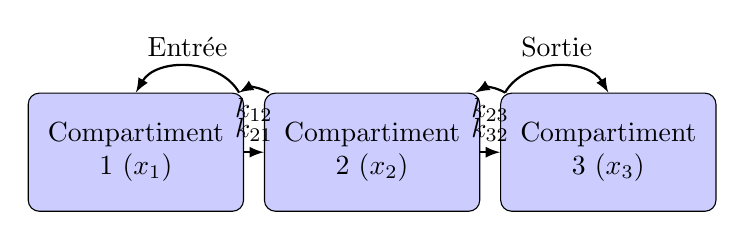
\begin{tikzpicture}[
            node distance=3cm,
            compartment/.style={rectangle, draw, fill=blue!20, rounded corners, minimum height=1.5cm, minimum width=2.5cm, text width=2.5cm, align=center},
            arrow/.style={-latex, thick}
        ]
            \node[compartment] (C1) {Compartiment 1 ($x_1$)};
            \node[compartment, right of=C1] (C2) {Compartiment 2 ($x_2$)};
            \node[compartment, right of=C2] (C3) {Compartiment 3 ($x_3$)};

            \draw[arrow] (C1) -- node[above] {$k_{21}$} (C2);
            \draw[arrow] (C2) -- node[above] {$k_{32}$} (C3);
            \draw[arrow] (C2) to[bend right] node[below] {$k_{12}$} (C1);
            \draw[arrow] (C3) to[bend right] node[below] {$k_{23}$} (C2);
            \draw[arrow] (C1) to[bend right=60] node[above] {Entrée} (C1.north);
            \draw[arrow] (C3) to[bend left=60] node[above] {Sortie} (C3.north);
        \end{tikzpicture}
    \end{center}
    \vfill
    \small{\textbf{Hypothèse clé:} La population dans chaque compartiment est instantanément et parfaitement mélangée}
\end{frame}

\begin{frame}{Histoire ancienne des idées compartimentales}
    \begin{itemize}
        \item \textbf{Début du XXe siècle:} Origines en cinétique chimique et épidémiologie
        \begin{itemize}
            \item \textbf{Ross (1911):} A modélisé la transmission du paludisme
            \item \textbf{Kermack \& McKendrick (1927):} Ont développé le modèle SIR fondateur pour les épidémies
        \end{itemize}
        \item \textbf{Milieu du XXe siècle:} Formalisation et application en pharmacocinétique et physiologie
        \item \textbf{John A. Jacquez (1922-2002):} Un pionnier de la théorie mathématique des systèmes compartimentaux
        \begin{itemize}
            \item Auteur du texte fondateur \textit{"Compartmental Analysis in Biology and Medicine"}
            \item A formalisé les concepts de spécification de modèle, d'identifiabilité structurelle et de propriétés des systèmes linéaires
        \end{itemize}
        \item \textbf{Carl P. Simon:} A travaillé extensivement sur l'analyse qualitative des systèmes dynamiques non linéaires, incluant les modèles épidémiologiques
        \begin{itemize}
            \item A contribué significativement à la compréhension de la stabilité des équilibres et des phénomènes de seuil dans la dynamique des maladies
        \end{itemize}
        \item \textbf{G. G. Walter:} A étudié les propriétés structurelles des modèles compartimentaux, particulièrement l'identifiabilité
    \end{itemize}
\end{frame}

\begin{frame}{Applications à travers les disciplines}
    \begin{columns}
        \begin{column}{0.5\textwidth}
            \textbf{Épidémiologie}
            \begin{itemize}
                \item Modélisation de la propagation des maladies infectieuses (SIR, SEIR)
                \item Évaluation des stratégies de vaccination
                \item Prédiction des trajectoires pandémiques (par ex., COVID-19)
            \end{itemize}
            \vspace{1cm}
            \textbf{Pharmacologie}
            \begin{itemize}
                \item Pharmacocinétique (PK) et Pharmacodynamique (PD)
                \item Absorption, distribution, métabolisme et excrétion des médicaments (ADME)
                \item Conception de schémas posologiques
            \end{itemize}
        \end{column}
        \begin{column}{0.5\textwidth}
            \textbf{Écologie}
            \begin{itemize}
                \item Cycle des nutriments dans les écosystèmes
                \item Dynamique des populations
                \item Flux de toxines dans les réseaux trophiques
            \end{itemize}
            \vspace{1cm}
            \textbf{Autres domaines}
            \begin{itemize}
                \item Génie chimique (modèles de réacteurs)
                \item Économie (flux de capitaux)
                \item Cinétique des traceurs en physiologie
            \end{itemize}
        \end{column}
    \end{columns}
\end{frame}


%%%%%%%%%%%%%%%%%%%%
%%%%%%%%%%%%%%%%%%%%
\Ssubsection{Fondamentaux de la modélisation compartimentale}{FIGS-slides-admin/Gemini_Generated_Image_k5h4qlk5h4qlk5h4.png}

\begin{frame}{Les éléments de base}
    \begin{itemize}
        \item \textbf{Compartiments ($C_i$):} Sous-populations ou quantités de matière.
        \begin{itemize}
            \item Exemple: Individus Susceptibles (S), Infectés (I), Rétablis (R).
        \end{itemize}
        \item \textbf{Variables d'état ($x_i(t)$):} La quantité ou concentration de matière dans le compartiment $i$ au temps $t$. L'état du système est le vecteur $\vect{x}(t) = [x_1(t), x_2(t), \dots, x_n(t)]^T$.
        \item \textbf{Flux (Fluxes):} Le taux de transfert de matière entre compartiments ou entre un compartiment et le monde extérieur (environnement).
        \begin{itemize}
            \item Soit $f_{ij}$ le taux de flux du compartiment $j$ vers le compartiment $i$.
            \item $f_{0j}$ est le taux de flux du compartiment $j$ vers l'environnement (excrétion/sortie).
            \item $f_{i0}$ est le taux de flux de l'environnement vers le compartiment $i$ (entrée).
        \end{itemize}
        \item \textbf{Constantes de taux ($k_{ij}$):} Paramètres qui déterminent le taux de flux. Dans les modèles linéaires, $f_{ij} = k_{ij} x_j$.
    \end{itemize}
\end{frame}

\begin{frame}{Formulation mathématique: le système EDO}
    La dynamique d'un système compartimental est décrite par un système d'équations différentielles ordinaires (EDO) du premier ordre.

    \begin{block}{Équation fondamentale de bilan}
        Pour chaque compartiment $i$, le taux de changement de sa variable d'état $x_i$ est donné par:
        $$ \frac{dx_i}{dt} = (\text{Somme de tous les flux entrants dans } C_i) - (\text{Somme de tous les flux sortants de } C_i) $$
    \end{block}

    Mathématiquement, pour un système à $n$ compartiments:
    $$ \frac{dx_i}{dt} = f_{i0}(t) + \sum_{j=1, j\neq i}^{n} f_{ij}(\vect{x}) - \sum_{j=0, j\neq i}^{n} f_{ji}(\vect{x}) $$
    où:
    \begin{itemize}
        \item $f_{i0}(t)$ est l'entrée dans le compartiment $i$.
        \item $f_{ij}(\vect{x})$ est le flux de $j$ vers $i$.
        \item $f_{ji}(\vect{x})$ est le flux de $i$ vers $j$.
        \item $f_{0i}(\vect{x})$ est l'excrétion du compartiment $i$.
    \end{itemize}
\end{frame}

\begin{frame}{Exemple: un modèle simple à deux compartiments}
    Considérons un système où un médicament est injecté dans le sang (Compartiment 1) puis se déplace vers les tissus (Compartiment 2) et est également éliminé du sang.

    \begin{center}
        \begin{tikzpicture}[
            node distance=4cm,
            compartment/.style={rectangle, draw, fill=green!20, rounded corners, minimum height=1.5cm, minimum width=3cm, text width=3cm, align=center},
            arrow/.style={-latex, thick}
        ]
            \node (env_in) [label=above:Entrée $I(t)$] {};
            \node[compartment, below=1cm of env_in] (C1) {Sang ($x_1$)};
            \node[compartment, right of=C1] (C2) {Tissus ($x_2$)};
            \node (env_out) [below=1cm of C1, label=below:Élimination] {};

            \draw[arrow] (env_in) -- (C1);
            \draw[arrow] (C1) to[bend left] node[above] {$k_{21}$} (C2);
            \draw[arrow] (C2) to[bend left] node[below] {$k_{12}$} (C1);
            \draw[arrow] (C1) -- node[left] {$k_{01}$} (env_out);
        \end{tikzpicture}
    \end{center}

    En supposant une cinétique linéaire du premier ordre ($f_{ij} = k_{ij}x_j$):
    \begin{align*}
        \frac{dx_1}{dt} &= I(t) + k_{12}x_2 - k_{21}x_1 - k_{01}x_1 \\
        \frac{dx_2}{dt} &= k_{21}x_1 - k_{12}x_2
    \end{align*}
\end{frame}

\begin{frame}{Modèles linéaires vs. non linéaires}
    \begin{columns}
        \begin{column}{0.5\textwidth}
            \textbf{Modèles compartimentaux linéaires}
            \begin{itemize}
                \item Tous les taux de flux $f_{ij}$ sont des fonctions linéaires des variables d'état: $f_{ij} = k_{ij}x_j$.
                \item Le système d'EDO est linéaire:
                $$ \frac{d\vect{x}}{dt} = A\vect{x} + \vect{b}(t) $$
                \item $A$ est la matrice compartimentale.
                \item Analytiquement traitable.
                \item Courant en cinétique des traceurs et en pharmacocinétique.
            \end{itemize}
        \end{column}
        \begin{column}{0.5\textwidth}
            \textbf{Modèles compartimentaux non linéaires}
            \begin{itemize}
                \item Au moins un taux de flux $f_{ij}$ est une fonction non linéaire des variables d'état.
                \item Exemple: $f_{ij} = \frac{V_{max} x_j}{K_m + x_j}$ (cinétique de Michaelis-Menten) ou $f_{ij} = \beta x_i x_j$ (action de masse, comme en épidémiologie).
                \item Le système d'EDO est non linéaire.
                \item Nécessite souvent des méthodes numériques et une analyse qualitative.
                \item Essentiel pour modéliser la dynamique des populations, l'épidémiologie et la cinétique enzymatique.
            \end{itemize}
        \end{column}
    \end{columns}
    \vfill
    \begin{alertblock}{Distinction clé}
        La nature du modèle (linéaire vs. non linéaire) dicte les outils mathématiques disponibles pour son analyse
    \end{alertblock}
\end{frame}

%%%%%%%%%%%%%%%%%%%%
%%%%%%%%%%%%%%%%%%%%
\Ssubsection{Propriétés mathématiques fondamentales}{FIGS-slides-admin/Gemini_Generated_Image_k5h4qlk5h4qlk5h4.png}

\begin{frame}{L'espace d'état et la positivité}
    \begin{definition}[Espace d'état]
        L'espace d'état est l'ensemble de toutes les valeurs possibles que le vecteur d'état $\vect{x}(t)$ peut prendre.
    \end{definition}
    \vfill
    Pour les modèles compartimentaux, les variables d'état représentent des quantités physiques (par ex., concentrations, populations), qui ne peuvent pas être négatives
    \vfill
    Par conséquent, l'espace d'état physiquement significatif est l'orthant non négatif:
    $$ \Omega = \IRplus^n = \{ \vect{x} \in \IR^n : x_i \ge 0 \text{ pour tout } i=1, \dots, n \} $$
    \vfill
    \begin{block}{Positivité des solutions}
        Une propriété cruciale d'un modèle compartimental bien posé est que si le système commence avec des conditions initiales non négatives, $\vect{x}(0) \in \Omega$, alors la solution $\vect{x}(t)$ doit rester dans $\Omega$ pour tout $t > 0$. Ceci est également connu comme l'\textbf{invariance progressive} de $\IRplus^n$.
    \end{block}
\end{frame}

\begin{frame}{Condition pour la positivité des solutions}
    \begin{theorem}[Condition de positivité, souvent attribuée à Jacquez]
        Considérons le système $\frac{d\vect{x}}{dt} = \vect{f}(\vect{x})$ avec $\vect{x}(0) \ge 0$. L'orthant non négatif $\IRplus^n$ est progressivement invariant si et seulement si pour chaque $i=1, \dots, n$:
        $$ f_i(\vect{x}) \ge 0 \quad \text{lorsque} \quad \vect{x} \in \IRplus^n \text{ et } x_i=0. $$
    \end{theorem}
    \vfill
    \textbf{Interprétation:}
    \begin{itemize}
        \item Si un compartiment est vide ($x_i=0$), le flux net entrant doit être non négatif
        \item En d'autres termes, on ne peut pas avoir un flux net \textit{sortant} d'un compartiment vide
        \item Pour les modèles linéaires $\frac{d\vect{x}}{dt} = A\vect{x}$, cette condition est équivalente à exiger que tous les éléments hors diagonale de la matrice compartimentale $A$ soient non négatifs ($a_{ij} \ge 0$ pour $i \neq j$)
    \end{itemize}
\end{frame}

\begin{frame}{La matrice compartimentale (cas linéaire)}
    Pour un système linéaire $\frac{d\vect{x}}{dt} = A\vect{x}$, la matrice $A$ a des propriétés spéciales.
    $$ \frac{dx_i}{dt} = \sum_{j=1, j \neq i}^{n} k_{ij}x_j - \left(k_{0i} + \sum_{j=1, j \neq i}^{n} k_{ji}\right)x_i $$
    Les éléments de $A = [a_{ij}]$ sont:
    \begin{itemize}
        \item \textbf{Éléments hors diagonale:} $a_{ij} = k_{ij} \ge 0$ pour $i \neq j$. (Ceci assure la positivité).
        \item \textbf{Éléments diagonaux:} $a_{ii} = -k_{0i} - \sum_{j=1, j \neq i}^{n} k_{ji} \le 0$. L'élément diagonal $a_{ii}$ représente le flux fractionnaire total sortant du compartiment $i$.
    \end{itemize}
    \vfill
    \begin{definition}[Matrice de Metzler]
        Une matrice avec des éléments hors diagonale non négatifs est appelée une matrice de Metzler. Toutes les matrices compartimentales linéaires sont des matrices de Metzler.
    \end{definition}
    Cette structure a des implications profondes pour la stabilité et le comportement du système.
\end{frame}

\begin{frame}{Conservation de la masse}
    \begin{definition}[Système fermé]
        Un système compartimental est \textbf{fermé} s'il n'y a pas de flux vers ou depuis l'environnement. C'est-à-dire, $f_{i0} = 0$ et $f_{0j} = 0$ pour tous $i, j$.
    \end{definition}
    \vfill
    \begin{theorem}[Conservation de la masse]
        Dans un système fermé, la quantité totale de matière est conservée.
        $$ \frac{d}{dt} \sum_{i=1}^n x_i = \sum_{i=1}^n \frac{dx_i}{dt} = 0 $$
        Par conséquent, $\sum_{i=1}^n x_i(t) = N$ (une constante) pour tout $t$.
    \end{theorem}
    \vfill
    \textbf{Esquisse de preuve:}
    $\sum_i \dot{x}_i = \sum_i \sum_{j \neq i} (f_{ij} - f_{ji})$. Puisque chaque flux $f_{ij}$ de $j$ vers $i$ est aussi un flux sortant de $j$, les termes s'annulent par paires.
    \vfill
    \textbf{Implication:} Pour les systèmes fermés comme de nombreux modèles épidémiologiques de base (par ex., SIR), la population totale $N = S(t) + I(t) + R(t)$ est constante. Ceci réduit la dimensionnalité du système.
\end{frame}

\begin{frame}{Exemple épidémiologique: Le modèle SIR}
    Un exemple classique de modèle compartimental fermé et non linéaire.
    \begin{itemize}
        \item \textbf{S:} Individus susceptibles
        \item \textbf{I:} Individus infectieux
        \item \textbf{R:} Individus rétablis (et immunés)
    \end{itemize}

    \begin{center}
        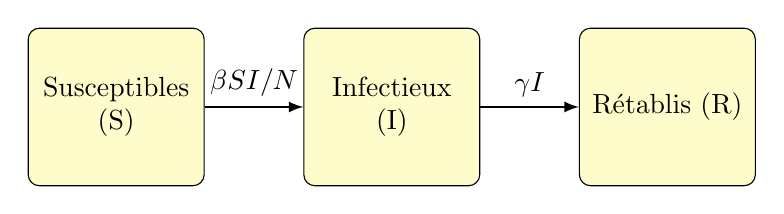
\begin{tikzpicture}[
            node distance=3.5cm,
            compartment/.style={rectangle, draw, fill=yellow!20, rounded corners, minimum size=2cm, text width=2cm, align=center},
            arrow/.style={-latex, thick}
        ]
            \node[compartment] (S) {Susceptibles (S)};
            \node[compartment, right of=S] (I) {Infectieux (I)};
            \node[compartment, right of=I] (R) {Rétablis (R)};

            \draw[arrow] (S) -- node[above] {$\beta SI/N$} (I);
            \draw[arrow] (I) -- node[above] {$\gamma I$} (R);
        \end{tikzpicture}
    \end{center}

    \textbf{Le système EDO:}
    \begin{align*}
        \frac{dS}{dt} &= -\frac{\beta S I}{N} \quad &\text{(Terme non linéaire: action de masse)} \\
        \frac{dI}{dt} &= \frac{\beta S I}{N} - \gamma I \\
        \frac{dR}{dt} &= \gamma I
    \end{align*}
    Ici, $S(t)+I(t)+R(t) = N$ est constant. L'espace d'état est le simplexe $\Delta = \{(S,I,R) \in \IRplus^3 : S+I+R=N\}$.
\end{frame}

%%%%%%%%%%%%%%%%%%%%
%%%%%%%%%%%%%%%%%%%%
\Ssubsection{Analyse des modèles compartimentaux linéaires}{FIGS-slides-admin/Gemini_Generated_Image_k5h4qlk5h4qlk5h4.png}

\begin{frame}{La forme matricielle et la solution}
    Un système compartimental linéaire invariant dans le temps peut s'écrire:
    $$ \frac{d\vect{x}}{dt} = A\vect{x}(t), \quad \vect{x}(0) = \vect{x}_0 $$
    où $A$ est la matrice compartimentale $n \times n$.

    \begin{block}{La solution générale}
        La solution de ce système est donnée par l'exponentielle matricielle:
        $$ \vect{x}(t) = e^{At} \vect{x}_0 $$
        où $e^{At} = \sum_{k=0}^{\infty} \frac{(At)^k}{k!}$.
    \end{block}

    Les propriétés de la solution $\vect{x}(t)$ sont déterminées par les valeurs propres et vecteurs propres de la matrice $A$.
\end{frame}

\begin{frame}{Valeurs propres et stabilité (Contribution de Jacquez)}
    \begin{theorem}[Application du théorème des cercles de Gershgorin]
        Soit $A$ une matrice compartimentale. Les valeurs propres $\lambda$ de $A$ se trouvent dans l'union des disques de Gershgorin dans le plan complexe:
        $$ D_i = \left\{ z \in \mathbb{C} : |z - a_{ii}| \le \sum_{j \neq i} |a_{ij}| = \sum_{j \neq i} a_{ij} \right\} $$
    \end{theorem}
    Puisque $a_{ii} = -k_{0i} - \sum_{j \neq i} k_{ji}$ et $a_{ij} = k_{ij}$ pour $j \neq i$:
    $$ a_{ii} = -k_{0i} - \sum_{j \neq i} a_{ji} $$
    La somme des éléments hors diagonale dans une colonne est $\sum_{j \neq i} a_{ji}$. La diagonale est $a_{ii}$. La somme de colonne est $\sum_{j=1}^n a_{ji} = -k_{0i} \le 0$.

    \begin{theorem}[Propriétés des valeurs propres de A, d'après Jacquez]
        Soit $A$ une matrice compartimentale. Alors:
        \begin{enumerate}
            \item Les parties réelles de toutes les valeurs propres de $A$ sont non positives ($\text{Re}(\lambda) \le 0$).
            \item Si le système a une "sortie" (c'est-à-dire, il existe un chemin de chaque compartiment vers l'environnement, rendant le graphe du système fortement connecté à l'environnement), alors toutes les valeurs propres ont des parties réelles strictement négatives ($\text{Re}(\lambda) < 0$). Dans ce cas, l'origine est un équilibre globalement asymptotiquement stable.
            \item Si le système est fermé, alors $\lambda=0$ est une valeur propre, et toutes les autres valeurs propres ont des parties réelles négatives. Le vecteur propre pour $\lambda=0$ correspond à une distribution d'état stationnaire.
        \end{enumerate}
    \end{theorem}
\end{frame}

\begin{frame}{Interprétation physique des valeurs propres}
    La solution $\vect{x}(t)$ peut s'exprimer comme une somme de modes correspondant aux valeurs propres:
    $$ \vect{x}(t) = \sum_{i=1}^n c_i \vect{v}_i e^{\lambda_i t} $$
    (en supposant des valeurs propres distinctes pour simplifier).
    \begin{itemize}
        \item Chaque $\lambda_i$ détermine une constante de temps du système, $\tau_i = -1/\text{Re}(\lambda_i)$.
        \item Les valeurs propres représentent les taux intrinsèques auxquels le système retourne à l'équilibre après une perturbation.
        \item Les modes plus rapides (grand $\text{Re}(\lambda_i)$ négatif) décroissent rapidement.
        \item Les modes plus lents (petit $\text{Re}(\lambda_i)$ négatif) dominent le comportement à long terme.
        \item Les parties imaginaires des valeurs propres correspondent à un comportement oscillatoire. Pour les modèles compartimentaux, les oscillations sont amorties.
    \end{itemize}
\end{frame}

\begin{frame}{Propriétés structurelles: Atteignabilité et observabilité}
    Ces concepts de la théorie du contrôle ont été appliqués à l'analyse compartimentale, notamment par Jacquez. Ils concernent ce qui peut être connu et contrôlé du système.

    \begin{definition}[Atteignabilité]
        Un état est \textbf{atteignable} s'il peut être atteint depuis l'origine en temps fini en utilisant une fonction d'entrée $\vect{b}(t)$. Un système est complètement atteignable si tous les états sont atteignables.
    \end{definition}
    \textbf{Question:} Pouvons-nous conduire le système à n'importe quel état désiré (par ex., concentration de médicament) avec une entrée externe?

    \begin{definition}[Observabilité]
        Un système est \textbf{observable} si, pour tout état initial $\vect{x}(0)$, il est possible de déterminer cet état à partir de l'historique de la sortie $\vect{y}(t) = C\vect{x}(t)$. La matrice $C$ définit quels compartiments sont mesurés.
    \end{definition}
    \textbf{Question:} Pouvons-nous déduire l'état de tous les compartiments en ne mesurant que quelques-uns?
\end{frame}

\begin{frame}{Identifiabilité structurelle (Contribution de Walter et Jacquez)}
    Un problème plus fondamental en modélisation.
    \begin{definition}[Identifiabilité structurelle]
        Un modèle est \textbf{structurellement identifiable} si ses paramètres inconnus peuvent être déterminés de manière unique à partir de données entrée-sortie parfaites (sans bruit), étant donnée la structure du modèle.
    \end{definition}

    \textbf{Le problème:}
    \begin{itemize}
        \item Nous proposons une structure de modèle (par ex., le diagramme à 2 compartiments).
        \item Nous ne pouvons qu'injecter un traceur (entrée) et mesurer sa concentration dans un compartiment (sortie).
        \item Pouvons-nous trouver de manière unique les valeurs de toutes les constantes de taux ($k_{ij}$) à partir de cette expérience?
    \end{itemize}
    \vfill
    \begin{alertblock}{Pourquoi c'est important}
        Si un modèle n'est pas structurellement identifiable, différents ensembles de valeurs de paramètres peuvent produire exactement la même sortie. Cela signifie que la structure interne du modèle est ambiguë et que les paramètres sont biologiquement sans signification.
    \end{alertblock}
    \vfill
    \small{G.G. Walter a fourni plusieurs conditions et théorèmes graphiques pour déterminer l'identifiabilité à partir du diagramme du modèle.}
\end{frame}

\begin{frame}{Exemple: Un modèle non identifiable}
    Considérons ce système "caténaire" où nous entrons dans C1 et observons C1.
    \begin{center}
        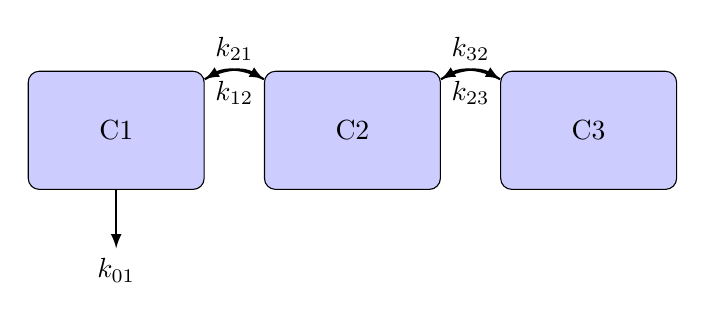
\begin{tikzpicture}[
            node distance=3cm,
            compartment/.style={rectangle, draw, fill=blue!20, rounded corners, minimum size=1.5cm, text width=2cm, align=center},
            arrow/.style={-latex, thick}
        ]
            \node[compartment] (C1) {C1};
            \node[compartment, right of=C1] (C2) {C2};
            \node[compartment, right of=C2] (C3) {C3};

            \draw[arrow] (C1) to[bend left] node[above] {$k_{21}$} (C2);
            \draw[arrow] (C2) to[bend right] node[below] {$k_{12}$} (C1);
            \draw[arrow] (C2) to[bend left] node[above] {$k_{32}$} (C3);
            \draw[arrow] (C3) to[bend right] node[below] {$k_{23}$} (C2);
            \draw[arrow] (C1) -- +(0,-1.5) node[below] {$k_{01}$};
        \end{tikzpicture}
    \end{center}
    La sortie de C1 est une somme d'exponentielles. Il s'avère que vous ne pouvez pas distinguer ce modèle de celui ci-dessous en n'observant que C1:
    \begin{center}
        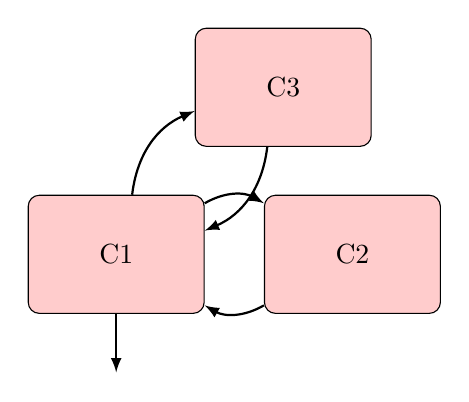
\begin{tikzpicture}[
            node distance=3cm,
            compartment/.style={rectangle, draw, fill=red!20, rounded corners, minimum size=1.5cm, text width=2cm, align=center},
            arrow/.style={-latex, thick}
        ]
            \node[compartment] (C1) {C1};
            \node[compartment, right of=C1] (C2) {C2};
            \node[compartment, above right of=C1] (C3) {C3};

            \draw[arrow] (C1) to[bend left] (C2);
            \draw[arrow] (C2) to[bend left] (C1);
            \draw[arrow] (C1) to[bend left] (C3);
            \draw[arrow] (C3) to[bend left] (C1);
            \draw[arrow] (C1) -- +(0,-1.5);
        \end{tikzpicture}
    \end{center}
    Les paramètres ne sont pas uniquement identifiables. Le travail de Walter a fourni des moyens systématiques de vérifier cela avant de conduire des expériences.
\end{frame}

%%%%%%%%%%%%%%%%%%%%
%%%%%%%%%%%%%%%%%%%%
\Ssubsection{Analyse des modèles non linéaires: épidémiologie}{FIGS-slides-admin/Gemini_Generated_Image_k5h4qlk5h4qlk5h4.png}

\begin{frame}{Le besoin de non-linéarité}
    Les modèles linéaires supposent que les taux sont proportionnels au compartiment source uniquement. Cela échoue quand les interactions entre populations sont essentielles.
    \vfill
    \textbf{Épidémiologie:} Le taux de nouvelles infections dépend du produit du nombre de personnes susceptibles et du nombre de personnes infectieuses.
    $$ \text{Taux de nouvelles infections} \propto S \times I $$
    Ceci est un terme \textbf{bilinéaire}, rendant le système non linéaire.
    \vfill
    \textbf{Conséquences de la non-linéarité:}
    \begin{itemize}
        \item Pas de solution analytique générale.
        \item Existence de multiples équilibres.
        \item Comportements complexes comme des seuils, bifurcations et cycles limites.
        \item L'analyse repose sur la théorie qualitative des systèmes dynamiques.
    \end{itemize}
\end{frame}

\begin{frame}{Équilibres et stabilité}
    \begin{definition}[Équilibre]
        Un équilibre (ou état stationnaire, point fixe) du système $\frac{d\vect{x}}{dt} = \vect{f}(\vect{x})$ est un point $\vect{x}^*$ tel que $\vect{f}(\vect{x}^*) = \vect{0}$. À l'équilibre, le système ne change pas.
    \end{definition}
    \vfill
    Pour le modèle SIR ($\dot{S}=-\beta SI/N, \dot{I}=\beta SI/N - \gamma I, \dot{R}=\gamma I$):
    \begin{itemize}
        \item \textbf{Équilibre sans maladie (DFE):}
        Ceci correspond à l'absence de maladie. Nous posons $I=0$.
        $$ I^* = 0 \implies \dot{S}=0, \dot{I}=0, \dot{R}=0 $$
        Le DFE est tout point $(S, 0, R)$ où $S+R=N$. Nous le désignons typiquement par $E_0 = (N, 0, 0)$.
        \item \textbf{Équilibre endémique (EE):}
        Ceci correspond à la persistance de la maladie dans la population. Nous posons $\dot{I}=0$ avec $I \neq 0$.
        $$ \frac{\beta S^* I^*}{N} - \gamma I^* = 0 \implies \frac{\beta S^*}{N} = \gamma \implies S^* = \frac{\gamma N}{\beta} $$
        Cet équilibre n'existe que si $S^* < N$, ce qui a des implications majeures.
    \end{itemize}
\end{frame}

\begin{frame}{Analyse de stabilité locale: la Jacobienne}
    Pour déterminer si un équilibre $\vect{x}^*$ est stable, nous linéarisons le système autour de lui.
    Le comportement du système non linéaire près de $\vect{x}^*$ est approché par le système linéaire:
    $$ \frac{d\vect{z}}{dt} = J(\vect{x}^*) \vect{z}, \quad \text{où } \vect{z} = \vect{x} - \vect{x}^* $$
    $J(\vect{x}^*)$ est la \textbf{matrice Jacobienne} de $\vect{f}$ évaluée en $\vect{x}^*$:
    $$ J_{ij} = \frac{\partial f_i}{\partial x_j} \bigg|_{\vect{x}=\vect{x}^*} $$
    \begin{theorem}[Hartman-Grobman, simplifié]
        La stabilité de l'équilibre $\vect{x}^*$ est déterminée par les valeurs propres de $J(\vect{x}^*)$:
        \begin{itemize}
            \item Si toutes les valeurs propres ont des parties réelles \textbf{négatives}, $\vect{x}^*$ est localement asymptotiquement stable
            \item Si au moins une valeur propre a une partie réelle \textbf{positive}, $\vect{x}^*$ est instable
            \item Si certaines valeurs propres ont une partie réelle nulle, le test n'est pas concluant
        \end{itemize}
    \end{theorem}
\end{frame}

\begin{frame}{Stabilité globale et fonctions de Lyapunov}
    La stabilité locale ne nous renseigne que sur le comportement près d'un équilibre. La stabilité globale assure que le système converge vers l'équilibre depuis (presque) toute condition initiale
    \begin{definition}[Fonction de Lyapunov]
        Une fonction de Lyapunov $L(\vect{x})$ pour un équilibre $\vect{x}^*$ est une fonction scalaire qui est définie positive ($L(\vect{x})>0$ pour $\vect{x}\neq\vect{x}^*$, $L(\vect{x}^*)=0$) et dont la dérivée temporelle le long des trajectoires est semi-définie négative ($\frac{dL}{dt} \le 0$)
    \end{definition}
    \textbf{Analogie:} Une fonction de Lyapunov est comme l'"énergie" du système. Si l'énergie diminue toujours, le système doit éventuellement se stabiliser à son état d'énergie minimale (l'équilibre)
    \vfill
    Trouver une fonction de Lyapunov est un art, mais pour de nombreux modèles épidémiologiques, elles peuvent être construites pour prouver la stabilité globale soit du DFE (quand $R_0 < 1$) soit de l'EE (quand $R_0 > 1$). Cela fournit des garanties beaucoup plus fortes sur le comportement du système
\end{frame}

%%%%%%%%%%%%%%%%%%%%
%%%%%%%%%%%%%%%%%%%%
\Ssubsection{Sujets avancés et modernes}{FIGS-slides-admin/Gemini_Generated_Image_k5h4qlk5h4qlk5h4.png}

\begin{frame}{Modèles compartimentaux stochastiques}
    Les EDO sont déterministes: avec les mêmes conditions initiales, le résultat est toujours le même. La vraie vie est stochastique.
    \vfill
    \textbf{Sources d'aléatoire:}
    \begin{itemize}
        \item \textbf{Stochasticité démographique:} Aléatoire provenant d'événements individuels (naissances, décès, transmissions) étant discrets. Important dans les petites populations.
        \item \textbf{Stochasticité environnementale:} Fluctuations aléatoires des paramètres du modèle (par ex., $\beta(t)$ varie aléatoirement autour d'une moyenne).
    \end{itemize}
    \vfill
    \textbf{Approches de modélisation:}
    \begin{itemize}
        \item \textbf{Chaînes de Markov à temps continu (CTMC):} Le nombre d'individus dans chaque compartiment est un entier, et les transitions sont des événements probabilistes. C'est l'approche la plus détaillée.
        \item \textbf{Équations différentielles stochastiques (SDE):} Ajoutent un terme de bruit aux EDO. Une bonne approximation pour les grandes populations.
    \end{itemize}
    \vfill
    Les modèles stochastiques peuvent prédire la probabilité d'extinction de la maladie, la taille des épidémies et fournir des intervalles de confiance pour les prédictions.
\end{frame}

\begin{frame}{Modèles de réseaux et basés sur les agents}
    L'hypothèse "bien mélangée" est souvent irréaliste. Les gens interagissent au sein d'une structure de réseau social.
    \begin{itemize}
        \item \textbf{Modèles de réseaux:} Les individus sont des nœuds, et les contacts sont des arêtes. La maladie se propage le long du réseau.
        \begin{itemize}
            \item Peut capturer le rôle des "super-propagateurs" (hubs dans le réseau).
            \item La distribution des degrés du réseau influence fortement $R_0$ et la dynamique épidémique.
        \end{itemize}
        \item \textbf{Modèles basés sur les agents (ABM):} L'approche la plus détaillée. Chaque individu ("agent") est simulé avec ses propres attributs et comportements.
        \begin{itemize}
            \item Intensif en calcul.
            \item Peut incorporer des comportements humains complexes, la géographie et des structures sociales détaillées.
            \item Floute la ligne avec les modèles compartimentaux traditionnels mais peut être vu comme une micro-simulation dont émergent les dynamiques compartimentales.
        \end{itemize}
    \end{itemize}
\end{frame}

\begin{frame}{Assimilation de données et estimation de paramètres}
    Un modèle n'est aussi bon que ses paramètres.
    \begin{itemize}
        \item \textbf{Le problème inverse:} Étant donné des données du monde réel (par ex., nombres de cas quotidiens), quelles sont les valeurs de paramètres les plus probables ($\beta, \gamma, \dots$)?
        \item C'est un problème d'estimation statistique.
    \end{itemize}
    \vfill
    \textbf{Méthodes courantes:}
    \begin{itemize}
        \item \textbf{Ajustement par moindres carrés:} Minimise la différence entre la sortie du modèle et les données. Sujet à rester bloqué dans des minima locaux.
        \item \textbf{Inférence bayésienne (MCMC):} Une approche moderne et puissante. Traite les paramètres comme des variables aléatoires et trouve leur distribution de probabilité a posteriori étant donné les données.
        \begin{itemize}
            \item Fournit non seulement une estimation ponctuelle mais une mesure d'incertitude (intervalles crédibles) pour chaque paramètre.
            \item Peut incorporer des connaissances préalables sur les paramètres.
        \end{itemize}
    \end{itemize}
    C'est là que le travail théorique sur l'identifiabilité structurelle de Jacquez et Walter devient critiquement important en pratique.
\end{frame}

%%%%%%%%%%%%%%%%%%%%
%%%%%%%%%%%%%%%%%%%%
\Ssubsection{Conclusion}{FIGS-slides-admin/Gemini_Generated_Image_k5h4qlk5h4qlk5h4.png}

\begin{frame}{Résumé des concepts clés}
    \begin{itemize}
        \item Les \textbf{modèles compartimentaux} fournissent un cadre puissant pour comprendre les systèmes dynamiques en les simplifiant en sous-populations interagissantes.
        \item La fondation mathématique est un système d'\textbf{EDO}, qui peut être linéaire ou non linéaire.
        \item Les \textbf{modèles linéaires}, centraux au travail de Jacquez, sont analysés via la matrice compartimentale, ses valeurs propres, et les concepts d'identifiabilité et d'observabilité.
        \item Les \textbf{modèles non linéaires}, essentiels pour l'épidémiologie, sont analysés en utilisant les outils des systèmes dynamiques, comme mis en évidence par le travail de Simon.
        \item Le \textbf{nombre de reproduction de base ($R_0$)} est la quantité seuil fondamentale qui détermine si une maladie se propagera ou s'éteindra.
        \item Le domaine évolue pour inclure plus de réalisme à travers la \textbf{stochasticité, les réseaux et les paramètres variant dans le temps}.
    \end{itemize}
\end{frame}

%%%%%%%%%%%%%%%%%%%%
%%%%%%%%%%%%%%%%%%%%
%%%%%%%%%%%%%%%%%%%%
%%%%%%%%%%%%%%%%%%%%
\section{Modèles épidémiques de type Kermack-McKendrick}
\newSectionSlide{FIGS-slides-admin/Gemini_Generated_Image_vqpscpvqpscpvqps.jpeg}

\maxFrameImage{FIGS/KMK-title-page}
\nocite{KermackMcKendrick1927}

\begin{frame}{Quelle est la \emph{taille} d'une épidémie ?}
\bbullet 
Si nous nous intéressons à la possibilité qu'une épidémie se produise
\begin{itemize}
  \item Un pic épidémique a-t-il toujours lieu ?
  \item S'il a lieu, quelle est sa taille ?
\end{itemize}
\vfill
\bbullet Si une épidémie traverse une population, tout le monde est-il affecté/infecté ?
\end{frame}


%%%%%%%%%%%%%%%%%%%%
%%%%%%%%%%%%%%%%%%%%
\Ssubsection{Le modèle de Kermack-McKendrick (KMK)}{FIGS-slides-admin/Gemini_Generated_Image_vqpscpvqpscpvqps.jpeg}

\maxFrameImage{FIGS/KMK-model-in-paper}


\begin{frame}{Le modèle SIR de Kermack-McKendrick sans démographie}
\bbullet La période de temps considérée est suffisamment courte pour que la démographie puisse être négligée (on dit aussi que le modèle n'a \emph{pas de dynamique vitale})
\vfill
\bbullet Les individus sont soit \emph{susceptibles} à la maladie soit \emph{infectés} par (et \emph{infectieux} avec) la maladie
\vfill
\bbullet Après guérison ou décès de la maladie, les individus sont \emph{retirés} du compartiment infectieux ($R$)
\vfill
\bbullet L'incidence est de type \defword{action de masse} et prend la forme $\beta SI$
\end{frame}


\begin{frame}{Les variables d'état}
Nous formulons le modèle comme un système d'\defword{équations différentielles}
\vfill
Équations différentielles : les inconnues sont des \emph{fonctions} (au lieu de scalaires, comme dans les équations algébriques)
\vfill
Au temps $t\geq 0$ (on suppose typiquement que le temps commence à $t=0$, mais on pourrait aussi considérer $t\geq t_0>0$), les \defword{variables d'état}, dans le modèle actuel, sont les nombres d'individus qui sont
\begin{itemize}
\item susceptibles à la maladie : $S(t)$
\item infectés et infectieux avec la maladie : $I(t)$
\item retirés du compartiment infectieux : $R(t)$
\end{itemize}
\vfill
Souvent, nous omettons la dépendance en $t$ si elle n'est pas explicitement requise et écrivons $S,I,R$
\end{frame}



\begin{frame}{Important -- Fonctions d'incidence}
L'incidence est le taux auquel de nouveaux cas apparaissent, la fonction d'incidence décrit alors comment les contacts conduisent à de nouvelles infections
\vfill
S'il y a $S$ individus susceptibles et $I$ individus infectieux dans la population, nous utilisons une fonction de la forme
\[
f(S,I)
\]
La fonction peut aussi dépendre explicitement de la population totale $N$, c'est-à-dire $f(S,I,N)$
\vfill
Nous revenons aux fonctions d'incidence dans \href{no.se}{Conférence 06}
\vfill
Pour l'instant, sachez juste que les fonctions d'incidence les plus courantes sont
\begin{itemize}
\item \defword{incidence d'action de masse} $f(S,I,N)=\beta SI$
\item \defword{incidence standard} (ou \defword{proportionnelle}) $f(S,I,N)=\beta SI/N$
\end{itemize}
\end{frame}



\begin{frame}{Le modèle de Kermack-McKendrick}
Ce modèle est généralement appelé le \defword{modèle SIR de Kermack-McKendrick} (KMK) 
  \begin{align*}
    \frac{d}{dt}S(t) &= -\beta S(t)I(t) \\
    \frac{d}{dt}I(t) &= \beta S(t)I(t)-\gamma I(t) \\
    \frac{d}{dt}R(t) &= \gamma I(t) 
    \end{align*}  
\vfill
\begin{center}
  \begin{tikzpicture}[scale=1.25, transform shape]
    \node [circle, fill=green!50, text=black] (S) {$S(t)$};
    \node [circle, right=1.5cm of S, fill=red!90, text=black] (I) {$I(t)$};
    \node [circle, right=1.5cm of I, fill=blue!90, text=black] (R) {$R(t)$};
    %% Flows
    \path [line, very thick] (S) to node [midway, above] (TextNode) {$\beta S(t)I(t)$} (I);
    \path [line, very thick] (I) to node [midway, above] (TextNode) {$\gamma I(t)$} (R);
  \end{tikzpicture}    
\end{center}
\end{frame}



\begin{frame}{Le modèle de Kermack-McKendrick}
Comme indiqué, nous omettons souvent la dépendance en $t$ des variables d'état ; nous écrivons aussi $X':=dX(t)/dt$. Ainsi le modèle KMK s'écrit habituellement
\vfill
\begin{subequations}\label{sys:KMK}
  \begin{align}
    S\pprime &= -\beta SI \label{sys:KMK_dS} \\
    I\pprime &= \beta SI-\gamma I \label{sys:KMK_dI} \\
    R\pprime &= \gamma I \label{sys:KMK_dR}
    \end{align}  
\end{subequations}
\vfill
\begin{center}
  \begin{tikzpicture}[scale=1.5, transform shape]
    \node [circle, fill=green!50, text=black] (S) {$S$};
    \node [circle, right=1cm of S, fill=red!90, text=black] (I) {$I$};
    \node [circle, right=1cm of I, fill=blue!90, text=black] (R) {$R$};
    %% Flows
    \path [line, very thick] (S) to node [midway, above] (TextNode) {$\beta SI$} (I);
    \path [line, very thick] (I) to node [midway, above] (TextNode) {$\gamma I$} (R);
  \end{tikzpicture}    
\end{center}
\end{frame}

%%%%%%%%%%%%%%%%%%%%
%%%%%%%%%%%%%%%%%%%%
\subsection{Analyse mathématique de KMK}
\newSubSectionSlide{FIGS-slides-admin/Gemini_Generated_Image_vqpscpvqpscpvqps.jpeg}


\begin{frame}{Réduction du modèle}
  3 compartiments, mais lorsqu'on les considère en détail, nous remarquons que les \emph{retirés} n'ont pas d'influence directe sur la dynamique de $S$ ou $I$, dans le sens où $R$ n'apparaît pas dans \eqref{sys:KMK_dS} ou \eqref{sys:KMK_dI}
  \vfill
  De plus, la population totale (incluant les décédés qui sont aussi dans $R$) $N=S+I+R$ satisfait
  \[
  N\pprime=(S+I+R)'=0
  \]
  Ainsi, $N$ est constant et 
  \begin{equation}\label{eq:constant_population}
    S(t)+I(t)+R(t)=N_0,\quad t\geq 0.
  \end{equation}
  donc la dynamique de $R$ peut être déduite de $R=N-(S+I)$.
  Donc nous pouvons considérer
  \begin{subequations}\label{sys:KMK_2d}
    \begin{align}
      S\pprime &= -\beta SI \label{sys:KMK_2d_dS}\\
      I\pprime &= \beta SI-\gamma I  \label{sys:KMK_2d_dI}
      \end{align}
    \end{subequations}
\end{frame}

\begin{frame}{Équilibres}
  Considérons les équilibres de
  \begin{subequations}
    \begin{align}
      S\pprime &= -\beta SI 
      \tag{\ref{sys:KMK_2d_dS}} \\
      I\pprime &= (\beta S-\gamma)I  
      \tag{\ref{sys:KMK_2d_dI}}
    \end{align}
  \end{subequations}
\vfill
  De \eqref{sys:KMK_2d_dI}
  \begin{itemize}
    \item soit $S^\star=\gamma/\beta$ 
    \item soit $I^\star=0$
  \end{itemize}
  \vfill
  Substituons dans \eqref{sys:KMK_2d_dS}
  \begin{itemize}
    \item dans le premier cas, $(S^\star,I^\star)=(\gamma/\beta,0)$ 
    \item dans le second cas, tout $S^\star\geq 0$ est un EP
  \end{itemize}
  \vfill
  Le second cas est un \emph{problème} : la linéarisation habituelle ne fonctionne pas lorsqu'il y a un \emph{continuum} d'équilibres car les EP ne sont pas \emph{isolés}
\end{frame}

\begin{frame}{Quel est le problème avec les EP non isolés ?}
\begin{proposition}\label{prop:EP_KMK}
Le modèle SIR de Kermack-McKendrick \eqref{sys:KMK} a le continuum d'équilibres
\begin{equation}
\label{eq:DFE_KMK}
    E_0^\text{KMK}:=\left\{
    (S^\star,I^\star,R^\star)=(S_\infty,0,N_0-S_\infty),\quad S_\infty\in[0,N_0]
    \right\}
\end{equation}
\end{proposition}
\end{frame}

\begin{frame}{Preuve}
Considérons \eqref{sys:KMK} et commençons avec $I=I^\star=0$.
Substituons cette valeur dans \eqref{sys:KMK_dS} à l'équilibre, donnant $0 = -\gamma S^\star I^\star(=0)$, signifiant que toute valeur de $S^\star$ satisfait cette relation. De la conservation de la population totale \eqref{eq:constant_population}, l'équilibre $E_0^\text{KMK}$ prend la forme donnée par \eqref{eq:DFE_KMK}
\vfill
Considérons maintenant $S=S^\star=\gamma/\beta$. Substituer cette valeur dans \eqref{sys:KMK_dS} à l'équilibre donne $0 = -\gamma I^\star$, d'où il suit que $I^\star=0$, et, en utilisant la conservation de la population totale \eqref{eq:constant_population},
\begin{equation}\label{eq:DFE_KMK_tmp}
    (S^\star,I^\star,R^\star)=\left(
    \frac{\gamma}{\beta},0,N_0-\frac{\gamma}{\beta}
    \right)
\end{equation}
est un équilibre de \eqref{sys:KMK}. 
L'équilibre \eqref{eq:DFE_KMK_tmp} est biologiquement pertinent seulement quand $N_0-\gamma/\beta\geq 0$.
Notons que \eqref{eq:DFE_KMK} inclut \eqref{eq:DFE_KMK_tmp} lorsque ce dernier est biologiquement pertinent
\end{frame}

\begin{frame}
En adaptant légèrement les définitions dans \cite{HirschSmale1974}, considérons l'équation différentielle ordinaire
\begin{equation}\label{eq:ODE}
    x' = f(x)
\end{equation}
où $x(t)\in W$ et $f:W\to E$ est une fonction telle que les solutions de \eqref{eq:ODE} existent de façon unique, par ex., une fonction $C^1$, d'un ensemble ouvert $W$ de l'espace vectoriel $E$ dans $E$
\vfill
Notons $x(t,x_0)$ la solution de \eqref{eq:ODE} passant par la valeur initiale $x(t_0)=x_0$
\end{frame}

\begin{frame}
Un point $x^\star\in W$ est un \defword{équilibre} si $f(x^\star)=0$
\vfill
\begin{definition}[Équilibre localement stable]\label{def:LS_EP}
Un point d'équilibre $x^\star$ de \eqref{eq:ODE} est \defword{localement stable} (LS) si pour tout voisinage $\mathcal{N}(x^\star)$ de $x^\star$ dans $W$, il existe un voisinage $\mathcal{N}_1\subseteq\mathcal{N}(x^\star)$ de $x^\star$ tel que toute solution $x(t,x_0)$ avec $x_0\in\mathcal{N}_1$ est définie et dans $\mathcal{N}(x^\star)$ pour tout $t>t_0$
\end{definition}
\vfill
\begin{definition}[Équilibre localement asymptotiquement stable]
Si $\mathcal{N}_1$ peut être choisi de sorte qu'en plus des propriétés de la Définition~\ref{def:LS_EP}, $\lim_{t\to\infty}x(t,x_0)=x^\star$ pour tout $x_0\in\mathcal{N}_1$, alors $x^\star$ est \defword{localement asymptotiquement stable} (LAS)
\end{definition}
\end{frame}

\begin{frame}
Les DFE \eqref{eq:DFE_KMK} de \eqref{sys:KMK} ne sont pas \defword{isolés} : tout voisinage (ouvert) d'un équilibre contient une infinité d'autres équilibres
\vfill
\begin{center}
    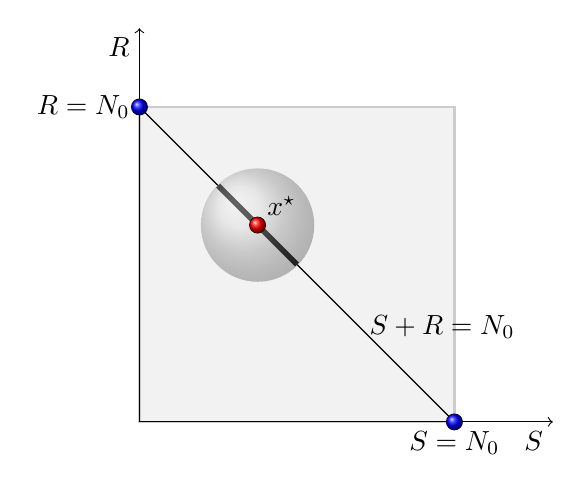
\begin{tikzpicture}
    \coordinate (SN) at (4,0);
    \coordinate (RN) at (0,4);
    \coordinate (xs) at (1.5,2.5);
    % The region
    \fill[gray!10] (0,4) -| (4,4) -| (4,0) -| (0,0) -- cycle;
    \draw[gray!40, thick]  (0,0) -- (4,0) -- (4,4) -- (0,4) -- cycle;
    % axis, on the top
    \draw[->] (0,0) -- (5.25,0) node[below left] {$S$};
    \draw[->] (0,0) -- (0,5) node[below left] {$R$};
    % The line of EP
    \draw[thin] (SN) -- (RN) node[pos=0.3,right] {$S+R=N_0$};
    \draw[line width=2] (1,3) -- (2,2);
    \shade[ball color = gray!40, opacity = 0.4] (xs) circle (0.72);
    % Intersections on S and R axes
    \draw (SN) circle (0.1cm) node[below] {$S=N_0$};
    \shade[ball color = blue, opacity = 1] (SN) circle (0.1cm);
    \draw (RN) circle (0.1cm) node[left] {$R=N_0$};
    \shade[ball color = blue, opacity = 1] (RN) circle (0.1cm);
    % The equilibrium
    \draw (xs) circle (0.1cm) node[above right] {$x^\star$};
    \shade[ball color = red, opacity = 1] (xs) circle (0.1cm);
    \end{tikzpicture}
\end{center}
\vfill
Voisinage $\N(x^\star)$ de $x^\star\in E_0^\text{KMK}$ se trouvant dans le plan $S-R$ (le voisinage s'étend au-dessus et en-dessous du plan $S-R$ dans la direction $I$, non montré ici). 
La ligne mince est $E_0^\text{KMK}$, la ligne épaisse est $E_0^\text{KMK}\cap\N(x^\star)$
\end{frame}

\begin{frame}
\begin{proposition}
Considérons un équilibre sans maladie $x^\star\in E_0^\text{KMK}$ de \eqref{sys:KMK}. Alors $x^\star$ est LS mais pas LAS  
\end{proposition}
\vfill
Cela signifie en particulier que considérer la matrice jacobienne de \eqref{sys:KMK} au DFE \textbf{n'a aucun sens} !
\end{frame}

\begin{frame}{Preuve}
Soit $x_1^\star\in E_0^\text{KMK}$ un équilibre de \eqref{sys:KMK}.
Considérons $\S_\mathcal{N}(x_1^\star)\subset E_0^\text{KMK}$, sous-ensemble ouvert de $E_0^\text{KMK}$ contenant $x_1^\star$.
Prenons maintenant un certain $x_2^\star\in\S_\mathcal{N}(x_1^\star)$. Puisque $x_2^\star\in\S_\mathcal{N}(x_1^\star)\subset E_0^\text{KMK}$, $x_2^\star$ est un équilibre de \eqref{sys:KMK} et donc $x(t,x_2^\star)=x_2^\star\in\S_\mathcal{N}(x_1^\star)$ pour tout $t\geq t_0$.
En conséquence, $x_1^\star$ est localement stable
\vfill
$\Rightarrow$ tout voisinage ouvert $\mathcal{N}(x_1^\star)$ contient $\S_\mathcal{N}=\mathcal{N}(x_1^\star)\cap E_0^\text{KMK}$
\vfill
Considérons alors un certain $x_2^\star\in\S_\mathcal{N}$.
Puisque $x_2^\star\in\S_\mathcal{N}$, $x_2^\star$ est un équilibre et en conséquence, $\lim_{t\to\infty}x(t,x_2^\star)=x_2^\star$.
Par conséquent, tout voisinage ouvert de $x_1^\star$ contient des points $x_0$ tels que $\lim_{t\to\infty}x(t,x_0)\neq x_1^\star$ $\implies$ $x_1^\star$ est LS mais pas LAS
\end{frame}

\begin{frame}{La méthode de la matrice de prochaine génération dans ce contexte}
Considérons la méthode de \cite{VdDWatmough2002}
\vfill
Pour construire $\R_0$, ils exigent la \emph{stabilité locale}
\vfill
Le Théorème 2 de \cite{VdDWatmough2002} concernant la LAS, d'autre part, a une hypothèse (hypothèse A5) selon laquelle le DFE doit être \emph{localement asymptotiquement stable}, avec l'hypothèse que toutes les valeurs propres de la linéarisation près d'un équilibre sans maladie ont des parties réelles négatives
\vfill
Clairement, ceci ne peut pas être vrai avec \eqref{sys:KMK}
\end{frame}


\begin{frame}{Une autre approche -- Étudier $dI/dS$}
  \begin{align}
  S\pprime &= -\beta SI \tag{\ref{sys:KMK_2d_dS}}\\
  I\pprime &= \beta SI-\gamma I  \tag{\ref{sys:KMK_2d_dI}}
  \end{align}
  \vfill
  Quelle est la dynamique de $dI/dS$ ? 
  \begin{equation}
    \label{eq:KMK_dI_over_dS}
    \frac{dI}{dS}
    =\frac{dI}{dt}\frac{dt}{dS}
    =\frac{I'}{S'}
    =\frac{\beta SI-\gamma I}{-\beta SI}
    =\frac{\gamma}{\beta S}-1
  \end{equation}
 pourvu que $S\neq 0$
  \vfill
  \textbf{Note --} Rappelons que $S$ et $I$ sont $S(t)$ et $I(t)$.. \eqref{eq:KMK_dI_over_dS} décrit donc la relation entre $S$ et $I$ le long des solutions de l'EDO originale \eqref{sys:KMK_2d}
\end{frame}


\begin{frame}{}
  Intégrer $\eqref{eq:KMK_dI_over_dS}$ et obtenir les trajectoires dans l'espace d'état
  $$
  I(S)=\frac\gamma\beta \ln S-S+C
  $$
  avec $C\in\IR$
  \vfill
  CI $I(S_0)=I_0$ $\Rightarrow$ $C=S_0+I_0-\dfrac \gamma\beta \ln S_0$ et la solution de \eqref{sys:KMK} est, en fonction de $S$
  \begin{align*}
  I(S)&=S_0+I_0-S+\frac\gamma\beta \ln \frac S{S_0} \\
  R(S)&=N-S-I(S)=R_0-\frac\gamma\beta \ln \frac S{S_0}
  \end{align*}
  (puisque $N_0=S_0+I_0+R_0$)
\end{frame}




\begin{frame}
Trajectoires de \eqref{sys:KMK_2d} dans l'espace $(S,I)$, normalisé, avec CI $(S_0,1-S_0)$ et $\beta/\gamma=2.5$
\vfill
\begin{center}
\includegraphics[width=0.9\textwidth]{FIGS/course-01-KMK_SI_plane-1.pdf}
\end{center}
\end{frame}



\begin{frame}{}
  Étudions
  $$
  I(S)=S_0+I_0-S+\frac\gamma\beta \ln \frac S{S_0} 
  $$
  Nous avons
  $$
  \frac{d}{dS}I(S) = \frac{\gamma}{\beta S}-1
  $$
  Ainsi, dans les courbes précédentes, le max de $I(S)$ se produit quand $S=\gamma/\beta$ ($S=0.4$ dans l'exemple)
  \vfill
  À ce point,
  $$
  I(S) = I_0+\left(
    1-\frac{1}{\R_0} - \frac{\ln(\R_0)}{\R_0}
  \right)S_0
  $$
\end{frame}


\begin{frame}{}
  \begin{theorem}[Epidemic or no epidemic?]
    Let $(S(t),I(t))$ be a solution to \eqref{sys:KMK_2d} and $\R_0$ defined by
    \begin{equation}\label{eq:R0_KMK}
    \R_0=\frac{\beta}{\gamma}S_0
    \end{equation}
    \vfill
    \begin{itemize}
      \item Si $\R_0\leq 1$, alors $I(t)\searrow 0$ quand $t\to\infty$ 
      \item Si $\R_0>1$, alors $I(t)$ atteint d'abord un maximum 
      \begin{equation}\label{eq:max_I}
        I_0+\left(
      1-\frac{1}{\R_0} - \frac{\ln(\R_0)}{\R_0}
      \right)S_0
      \end{equation}
      puis tend vers 0 quand $t\to\infty$  
    \end{itemize}    
  \end{theorem}
\end{frame}

\begin{knitrout}
\definecolor{shadecolor}{rgb}{0.969, 0.969, 0.969}\color{fgcolor}\begin{kframe}
\begin{alltt}
\hldef{rhs_SIR_KMK} \hlkwb{<-} \hlkwa{function}\hldef{(}\hlkwc{t}\hldef{,} \hlkwc{x}\hldef{,} \hlkwc{p}\hldef{) \{}
  \hlkwd{with}\hldef{(}\hlkwd{as.list}\hldef{(}\hlkwd{c}\hldef{(x, p)), \{}
    \hldef{dS} \hlkwb{=} \hlopt{-} \hldef{beta} \hlopt{*} \hldef{S} \hlopt{*} \hldef{I}
    \hldef{dI} \hlkwb{=} \hldef{beta} \hlopt{*} \hldef{S} \hlopt{*} \hldef{I} \hlopt{-} \hldef{gamma} \hlopt{*} \hldef{I}
    \hldef{dR} \hlkwb{=} \hldef{gamma} \hlopt{*} \hldef{I}
    \hlkwd{return}\hldef{(}\hlkwd{list}\hldef{(}\hlkwd{c}\hldef{(dS, dI, dR)))}
  \hldef{\})}
\hldef{\}}
\hlcom{# Initial condition for S (to compute R_0)}
\hldef{S0} \hlkwb{=} \hlnum{1000}
\hldef{gamma} \hlkwb{=} \hlnum{1}\hlopt{/}\hlnum{14}
\hlcom{# Set beta so that R_0 = 1.5}
\hldef{beta} \hlkwb{=} \hlnum{1.5} \hlopt{*} \hldef{gamma} \hlopt{/} \hldef{S0}
\hldef{params} \hlkwb{=} \hlkwd{list}\hldef{(}\hlkwc{gamma} \hldef{= gamma,} \hlkwc{beta} \hldef{= beta)}
\hldef{IC} \hlkwb{=} \hlkwd{c}\hldef{(}\hlkwc{S} \hldef{= S0,} \hlkwc{I} \hldef{=} \hlnum{1}\hldef{,} \hlkwc{R} \hldef{=} \hlnum{0}\hldef{)}
\hldef{times} \hlkwb{=} \hlkwd{seq}\hldef{(}\hlnum{0}\hldef{,} \hlnum{365}\hldef{,} \hlnum{1}\hldef{)}
\hldef{sol_KMK} \hlkwb{<-} \hlkwd{ode}\hldef{(IC, times, rhs_SIR_KMK, params)}
\end{alltt}
\end{kframe}
\end{knitrout}



\begin{frame}[fragile]{}
\begin{knitrout}
\definecolor{shadecolor}{rgb}{0.969, 0.969, 0.969}\color{fgcolor}\begin{kframe}
\begin{alltt}
\hlkwd{plot}\hldef{(sol_KMK[,} \hlsng{"time"}\hldef{], sol_KMK[,} \hlsng{"I"}\hldef{],}
     \hlkwc{type} \hldef{=} \hlsng{"l"}\hldef{,} \hlkwc{lwd} \hldef{=} \hlnum{2}\hldef{,}
     \hlkwc{main} \hldef{=} \hlkwd{TeX}\hldef{(}\hlsng{"Kermack-McKendrick SIR, $R_0=1.5$"}\hldef{),}
     \hlkwc{xlab} \hldef{=} \hlsng{"Time (days)"}\hldef{,} \hlkwc{ylab} \hldef{=} \hlsng{"Prevalence"}\hldef{)}
\end{alltt}
\end{kframe}
\end{knitrout}
\begin{center}
\includegraphics[width=0.8\textwidth]{FIGS/course-01-KMK_R0eq1dot5-1.pdf}
\end{center}
\end{frame}


\begin{frame}\frametitle{Le nombre de reproduction de base $\R_0$}
\bbullet Indicateur souvent utilisé en épidémiologie. Verbalement
\begin{quote}
  nombre moyen de cas secondaires d'infection produits lorsqu'un seul individu infectieux est introduit dans une population entièrement susceptible
\end{quote}
\vfill
\bbullet Si $\R_0<1$, alors chaque individu infectieux infecte en moyenne moins d'1 personne et l'épidémie a de fortes chances de s'éteindre 
\vfill
\bbullet Si $R_0>1$, alors chaque individu infectieux infecte en moyenne plus d'1 personne et une épidémie a de fortes chances de se produire
\end{frame}

\begin{frame}{Quelques valeurs types de $\R_0$}
  $\R_0$ can be estimated from data (from the Anderson \& May book)
  \vfill
  \begin{center}
  \begin{tabular}{llcc}
  \hline 
  Infection & Location & Period & $\R_0$ \\
  \hline
  Measles & Cirencester, England & 1947-50 & 13-14 \\
  & England and Wales & 1950-68 & 16-18 \\
  & Kansas, USA & 1918-21 & 5-6 \\
  & Ontario, Canada & 1912-3 & 11-12 \\
  & Willesden, England & 1912-3 & 11-12 \\
  & Ghana & 1960-8 & 14-15 \\
  & East Nigeria & 1960-8 & 16-17 \\
  \end{tabular}
  \end{center}
\end{frame}
    

%%%%%%%%%%%%%%%%%%%%%%%%
%%%%%%%%%%%%%%%%%%%%%%%%
\subsection{La taille finale d'une épidémie KMK}
\newSubSectionSlide{FIGS-slides-admin/Gemini_Generated_Image_vqpscpvqpscpvqps.jpeg}

\begin{frame}{Taille finale d'une épidémie}
  Pour une fonction intégrable à valeurs non négatives $w(t)$, notons
  $$
  w_0=w(0),\qquad  w_\infty = \lim_{t\to\infty}w(t),\qquad\hat w = \int_0^\infty w(t)\ dt
  $$
  \vfill
  Dans le sous-système
  \begin{align}
  S' &= -\beta SI \tag{\ref{sys:KMK_2d_dS}} \\
  I' &= \beta SI-\gamma I \tag{\ref{sys:KMK_2d_dI}} 
  \end{align}
  calculons la somme de \eqref{sys:KMK_2d_dS} et \eqref{sys:KMK_2d_dI}, en veillant à montrer la dépendance temporelle $$
  \frac{d}{dt}(S(t)+I(t))=-\gamma I(t)
  $$
\end{frame}


\begin{frame}{}
  Intégrons de 0 à $\infty$:
  $$
  \int_0^\infty\frac{d}{dt}(S(t)+I(t))\ dt=-\int_0^\infty\gamma I(t)dt 
  $$
  Le côté gauche donne
  $$
  \int_0^\infty\frac{d}{dt}(S(t)+I(t))\ dt
  = S_\infty+I_\infty-S_0-I_0 = S_\infty-S_0-I_0
  $$
  puisque $I_\infty=0$
  \vfill
  Le côté droit prend la forme
  $$
  -\int_0^\infty\gamma I(t)dt = -\gamma\int_0^\infty I(t)dt = -\gamma \hat I
  $$
  We thus have
  \begin{equation}
  \label{eq:KMK_final_size_step1}
  S_\infty-S_0-I_0 = -\gamma\hat I
  \end{equation}
\end{frame}



\begin{frame}{}
  Maintenant considérons \eqref{sys:KMK_2d_dS}:
  $$
  S' = -\beta SI
  $$
  Divisons les deux côtés par $S$:
  $$
  \frac{S'(t)}{S(t)} = -\beta I(t)
  $$
  Intégrons de 0 à $\infty$:
  \begin{equation}
  \label{eq:KMK_final_size_step2}
  \ln S_\infty-\ln S_0 = -\beta \hat I
  \end{equation}
  Express \eqref{eq:KMK_final_size_step1} and \eqref{eq:KMK_final_size_step2} in terms of $-\hat I$ and equate
  $$
  \frac{\ln S_\infty-\ln S_0}{\beta}
  =
  \frac{S_\infty-S_0-I_0}{\gamma}
  $$
  Thus we have
  \begin{equation}
  \label{eq:final_size}
  (\ln S_0-\ln S_\infty)S_0 = (S_0-S_\infty)\R_0+I_0\R_0
  \end{equation}
\end{frame}



\begin{frame}{}
\begin{theorem}[Final size relation]
  Let $(S(t),I(t))$ be a solution to \eqref{sys:KMK_2d} and $\R_0$ defined by \eqref{eq:R0_KMK}
  \vskip0.5cm
  The number $S(t)$ of susceptible individuals is a nonincreasing function and its limit $S_\infty$ is the only solution in $(0,S_0)$ of the transcendental equation
  \begin{equation}\tag{\ref{eq:final_size}}
  (\ln S_0-\ln S_\infty)S_0 = (S_0-S_\infty)\R_0+I_0\R_0
  \end{equation}
\end{theorem}
\end{frame}



\begin{frame}{L'équation (transcendante) de taille finale}
  Rewrite the final size equation
  \begin{equation}
    \tag{\ref{eq:final_size}}
  (\ln S_0-\ln S_\infty)S_0 = (S_0-S_\infty)\R_0+I_0\R_0
  \end{equation}
  as
  \begin{equation}
  \label{eq:final_size_2}
  T(S_\infty) =(\ln S_0-\ln S_\infty)S_0
  - (S_0-S_\infty)\R_0 -I_0\R_0
\end{equation}
\vfill
Ainsi, nous cherchons les zéros de la fonction $T(S_\infty)$
\end{frame}



\begin{frame}{}
  Nous cherchons $S_\infty$ dans $(0,S_0]$ t.q. $T(S_\infty)=0$, avec
  \begin{equation}\tag{\ref{eq:final_size_2}}
    T(S_\infty) =(\ln S_0-\ln S_\infty)S_0
    - (S_0-S_\infty)\R_0 -I_0\R_0      
  \end{equation}
  \vfill
  Notons pour commencer que 
  $$
  \lim_{S_\infty\to 0}T(S_\infty)=\lim_{S_\infty\to 0}-S_0\ln(S_\infty)=\infty
  $$
  \vfill
  En dérivant $T$ par rapport à $S_\infty$, nous obtenons 
  $$
  T'(S_\infty)=\R_0-S_0/S_\infty
  $$ 
  \vfill
  Quand $S_\infty\to 0$, $\R_0-S_0/S_\infty<0$, donc $T$ décroît jusqu'à $S_\infty=S_0/\R_0$
  \vfill
  Donc si $\R_0\leq 1$, la fonction $T$ est décroissante sur $(0,S_0)$, tandis qu'elle a un minimum si $\R_0>1$
\end{frame}



\begin{frame}{Cas $\R_0\leq 1$}
  \begin{equation}\tag{\ref{eq:final_size_2}}
    T(S_\infty) =(\ln S_0-\ln S_\infty)S_0
    - (S_0-S_\infty)\R_0 -I_0\R_0      
  \end{equation}
  \vfill
  \bbullet Nous avons vu que $T$ décroît sur $(0,S_0]$
  \vfill
  \bbullet Aussi, $T(S_0)=-I_0\R_0<0$ ($I_0=0$ est trivial et n'est pas considéré)
  \vfill
  \bbullet $T$ est continue
  \vfill
  $\implies$ il existe un unique $S_\infty\in (0,S_0]$ t.q. $T(S_\infty)=0$
\end{frame}


\begin{frame}{Cas $\R_0> 1$}
  \begin{equation}\tag{\ref{eq:final_size_2}}
    T(S_\infty) =(\ln S_0-\ln S_\infty)S_0
    - (S_0-S_\infty)\R_0 -I_0\R_0      
  \end{equation}
  \vfill
  \bbullet Nous avons vu que $T$ décroît sur $(0,S_0/\R_0]$
  \vfill
  \bbullet Pour $S_\infty\in[S_0/\R_0]$, $T'>0$
  \vfill
  \bbullet Comme avant, $T(S_\infty)=-I_0\R_0$
  \vfill
  \bbullet $T$ est continue
  \vfill
  $\implies$ il existe un unique $S_\infty\in (0,S_0]$ t.q. $T(S_\infty)=0$. Plus précisément, dans ce cas, $S_\infty\in(0,S_0/\R_0)$
\end{frame}



\begin{frame}[fragile]{}
Nous résolvons numériquement. Nous avons besoin d'une fonction
\begin{knitrout}
\definecolor{shadecolor}{rgb}{0.969, 0.969, 0.969}\color{fgcolor}\begin{kframe}
\begin{alltt}
\hldef{final_size_eq} \hlkwb{=} \hlkwa{function}\hldef{(}\hlkwc{S_inf}\hldef{,} \hlkwc{S0} \hldef{=} \hlnum{999}\hldef{,} \hlkwc{I0} \hldef{=} \hlnum{1}\hldef{,} \hlkwc{R_0} \hldef{=} \hlnum{2.5}\hldef{) \{}
  \hldef{OUT} \hlkwb{=} \hldef{S0}\hlopt{*}\hldef{(}\hlkwd{log}\hldef{(S0)}\hlopt{-}\hlkwd{log}\hldef{(S_inf))} \hlopt{-} \hldef{(S0}\hlopt{+}\hldef{I0}\hlopt{-}\hldef{S_inf)}\hlopt{*}\hldef{R_0}
  \hlkwd{return}\hldef{(OUT)}
\hldef{\}}
\end{alltt}
\end{kframe}
\end{knitrout}
et résolvons facilement en utilisant \code{uniroot}:
\begin{knitrout}
\definecolor{shadecolor}{rgb}{0.969, 0.969, 0.969}\color{fgcolor}\begin{kframe}
\begin{alltt}
\hlkwd{uniroot}\hldef{(}\hlkwc{f} \hldef{= final_size_eq,} \hlkwc{interval} \hldef{=} \hlkwd{c}\hldef{(}\hlnum{0.05}\hldef{,} \hlnum{999}\hldef{))}
\end{alltt}
\begin{verbatim}
## $root
## [1] 106.8819
## 
## $f.root
## [1] -2.649285e-07
## 
## $iter
## [1] 10
## 
## $init.it
## [1] NA
## 
## $estim.prec
## [1] 6.103516e-05
\end{verbatim}
\end{kframe}
\end{knitrout}
\end{frame}


\begin{frame}[fragile]{Une fonction pour utiliser ceci..}
\begin{knitrout}
\definecolor{shadecolor}{rgb}{0.969, 0.969, 0.969}\color{fgcolor}\begin{kframe}
\begin{alltt}
\hldef{final_size} \hlkwb{=} \hlkwa{function}\hldef{(}\hlkwc{L}\hldef{) \{}
  \hlkwd{with}\hldef{(}\hlkwd{as.list}\hldef{(L), \{}
  \hldef{S_inf} \hlkwb{=} \hlkwd{uniroot}\hldef{(}\hlkwc{f} \hldef{=} \hlkwa{function}\hldef{(}\hlkwc{x}\hldef{)}
    \hlkwd{final_size_eq}\hldef{(}\hlkwc{S_inf} \hldef{= x,}
                  \hlkwc{S0} \hldef{= S0,} \hlkwc{I0} \hldef{= I0,}
                  \hlkwc{R_0} \hldef{= R_0),}
    \hlkwc{interval} \hldef{=} \hlkwd{c}\hldef{(}\hlnum{0.05}\hldef{, S0))}
  \hlkwd{return}\hldef{(S_inf}\hlopt{$}\hldef{root)}
  \hldef{\})}
\hldef{\}}
\end{alltt}
\end{kframe}
\end{knitrout}
\end{frame}

\begin{frame}[fragile]{A figure with all the information}
\begin{knitrout}
\definecolor{shadecolor}{rgb}{0.969, 0.969, 0.969}\color{fgcolor}\begin{kframe}
\begin{alltt}
\hldef{N0} \hlkwb{=} \hlnum{1000}
\hldef{I0} \hlkwb{=} \hlnum{1}
\hldef{S0} \hlkwb{=} \hldef{N0}\hlopt{-}\hldef{I0}
\hldef{R_0} \hlkwb{=} \hlnum{0.8}
\hldef{S} \hlkwb{=} \hlkwd{seq}\hldef{(}\hlnum{0.1}\hldef{, S0,} \hlkwc{by} \hldef{=} \hlnum{0.1}\hldef{)}
\hldef{fs} \hlkwb{=} \hlkwd{final_size_eq}\hldef{(S,} \hlkwc{S0} \hldef{= S0,} \hlkwc{I0} \hldef{= I0,} \hlkwc{R_0} \hldef{= R_0)}
\hldef{S_inf} \hlkwb{=} \hlkwd{uniroot}\hldef{(}\hlkwc{f} \hldef{=} \hlkwa{function}\hldef{(}\hlkwc{x}\hldef{)} \hlkwd{final_size_eq}\hldef{(}\hlkwc{S_inf} \hldef{= x,}
                                              \hlkwc{S0} \hldef{= S0,} \hlkwc{I0} \hldef{= I0,}
                                              \hlkwc{R_0} \hldef{= R_0),}
                \hlkwc{interval} \hldef{=} \hlkwd{c}\hldef{(}\hlnum{0.05}\hldef{, S0))}
\hlkwd{plot}\hldef{(S, fs,} \hlkwc{type} \hldef{=} \hlsng{"l"}\hldef{,} \hlkwc{ylab} \hldef{=} \hlsng{"Value of equation (10)"}\hldef{)}
\hlkwd{abline}\hldef{(}\hlkwc{h} \hldef{=} \hlnum{0}\hldef{)}
\hlkwd{points}\hldef{(}\hlkwc{x} \hldef{= S_inf}\hlopt{$}\hldef{root,} \hlkwc{y} \hldef{=} \hlnum{0}\hldef{,} \hlkwc{pch} \hldef{=} \hlnum{19}\hldef{)}
\hlkwd{text}\hldef{(}\hlkwc{x} \hldef{= S_inf}\hlopt{$}\hldef{root,} \hlkwc{y} \hldef{=} \hlnum{0}\hldef{,} \hlkwc{labels} \hldef{=} \hlsng{"S_inf"}\hldef{,} \hlkwc{adj} \hldef{=} \hlkwd{c}\hldef{(}\hlopt{-}\hlnum{0.25}\hldef{,}\hlopt{-}\hlnum{1}\hldef{))}
\end{alltt}
\end{kframe}
\end{knitrout}
\end{frame}



\begin{frame}{$\R_0=0.8$}
\begin{center}
  \includegraphics[width=\textwidth]{FIGS/course-01-KMK_final_size_0p8-1.pdf}
\end{center}
\end{frame}





\begin{frame}{$\R_0=2.4$}
  \begin{center}
    \includegraphics[width=\textwidth]{FIGS/course-01-KMK_final_size_2p5-1.pdf}
  \end{center}
\end{frame}

\begin{frame}[fragile]{A little nicer}
\begin{knitrout}
\definecolor{shadecolor}{rgb}{0.969, 0.969, 0.969}\color{fgcolor}\begin{kframe}
\begin{alltt}
\hldef{values} \hlkwb{=} \hlkwd{expand.grid}\hldef{(}
  \hlkwc{R_0} \hldef{=} \hlkwd{seq}\hldef{(}\hlnum{0.01}\hldef{,} \hlnum{3}\hldef{,} \hlkwc{by} \hldef{=} \hlnum{0.01}\hldef{),}
  \hlkwc{I0} \hldef{=} \hlkwd{seq}\hldef{(}\hlnum{1}\hldef{,} \hlnum{100}\hldef{,} \hlnum{1}\hldef{)}
\hldef{)}
\hldef{values}\hlopt{$}\hldef{S0} \hlkwb{=} \hldef{N0}\hlopt{-}\hldef{values}\hlopt{$}\hldef{I0}
\hldef{L} \hlkwb{=} \hlkwd{split}\hldef{(values,} \hlnum{1}\hlopt{:}\hlkwd{nrow}\hldef{(values))}
\hldef{values}\hlopt{$}\hldef{S_inf} \hlkwb{=} \hlkwd{sapply}\hldef{(}\hlkwc{X} \hldef{= L,} \hlkwc{FUN} \hldef{= final_size)}
\hldef{values}\hlopt{$}\hldef{final_size} \hlkwb{=} \hldef{values}\hlopt{$}\hldef{S0}\hlopt{-}\hldef{values}\hlopt{$}\hldef{S_inf}\hlopt{+}\hldef{values}\hlopt{$}\hldef{I0}
\hldef{values}\hlopt{$}\hldef{attack_rate} \hlkwb{=} \hldef{(values}\hlopt{$}\hldef{final_size} \hlopt{/} \hldef{N0)}\hlopt{*}\hlnum{100}

\hldef{p} \hlkwb{=} \hlkwd{levelplot}\hldef{(attack_rate} \hlopt{~} \hldef{R_0}\hlopt{*}\hldef{I0,} \hlkwc{data} \hldef{= values,}
              \hlkwc{xlab} \hldef{=} \hlkwd{TeX}\hldef{(}\hlsng{"$R_0$"}\hldef{),} \hlkwc{ylab} \hldef{=} \hlsng{"I(0)"}\hldef{,}
              \hlkwc{col.regions} \hldef{=} \hlkwd{viridis}\hldef{(}\hlnum{100}\hldef{))}
\hlkwd{print}\hldef{(p)}
\end{alltt}
\end{kframe}
\end{knitrout}
(requires \code{lattice}, \code{viridis} and \code{latex2exp} librairies)
\end{frame}

\begin{frame}{Taux d'attaque (en \%)}
  \begin{center}
    \includegraphics[width=0.9\textwidth]{FIGS/course-01-KMK_attack_rate-1.pdf}
  \end{center}
\end{frame}


%%%%%%%%%%%%%%%%%%%%%%%%%%%
%%%%%%%%%%%%%%%%%%%%%%%%%%%
\subsection{Immunité collective dans KMK}
\newSubSectionSlide{FIGS-slides-admin/Gemini_Generated_Image_vqpscpvqpscpvqps.jpeg}


\begin{frame}{Le modèle de vaccination le plus simple}
Pour implémenter la vaccination dans KMK, supposons que la vaccination réduit le nombre de susceptibles
\vfill
Soit une population totale $N$ avec $S_0$ initialement susceptibles
\vfill
Vaccinons une fraction $p\in[0,1]$ des individus susceptibles
\vfill
CI originale (pour simplifier, $R(0)=0$)
\begin{equation}\label{eq:IC_KMK_novacc}
CI: (S(0),I(0),R(0)) = (S_0,I_0,0)
\end{equation}
CI post-vaccination 
\begin{equation}\label{eq:IC_KMK_vacc}
CI: (S(0),I(0),R(0)) = ((1-p)S_0,I_0,pS_0)
\end{equation}
\end{frame}


\begin{frame}{Nombre de reproduction avec vaccination}
  Without vaccination
  \begin{equation}\tag{\ref{eq:R0_KMK}}
    \R_0=\frac{\beta}{\gamma}S_0
  \end{equation}
  \vfill
  With vaccination, denoting $\R_{\text{v}}$ the reproduction number,
  \begin{equation}
    \R_{\text{v}} = \frac{\beta}{\gamma}(1-p)S_0
  \end{equation}
  \vfill
  Puisque $p\in[0,1]$, $\R_{\text{v}}\leq\R_0$
\end{frame}


\begin{frame}{Immunité collective}
  Par conséquent
  \begin{itemize}
    \item $\R_{\text{v}}<\R_0$ si $p>0$ 
    \item Pour contrôler la maladie, $\R_{\text{v}}$ doit prendre une valeur inférieure à 1
  \end{itemize}
  \vfill
Pour faire en sorte que $\R_{\text{v}}$ soit inférieur à 1
  \begin{equation}\label{eq:herd_immunity}
    \R_{\text{v}}<1 \iff p> 1-\frac{1}{\R_0}
  \end{equation}
  \vfill
  En vaccinant une fraction $p>1-1/\R_0$ de la population susceptible, nous sommes donc dans une situation où un pic épidémique est exclu (ou, à tout le moins, la taille finale est réduite)
  \vfill
  C'est l'\defword{immunité collective}
\end{frame}


%%%%%%%%%%%%%%%%%%%%%%%
%%%%%%%%%%%%%%%%%%%%%%%
\subsection{Le modèle SLIAR}
\newSubSectionSlide{FIGS-slides-admin/Gemini_Generated_Image_vqpscpvqpscpvqps.jpeg}

\maxFrameImage{FIGS/Arino-etal-SLIAR.png}
\nocite{ArinoBrauerPvdDWatmoughWu2006}

\begin{frame}
SIR est un peu trop simple pour de nombreuses maladies :
\vfill
\begin{itemize}
\item Pas de période d'incubation
\vfill
\item Beaucoup de maladies infectieuses (en particulier respiratoires) ont des formes légères et moins légères selon le patient
\end{itemize}
\vfill
$\implies$ modèle avec SIR mais aussi des individus L(atents) et (A)symptomatiques, dans lequel I sont maintenant des individus symptomatiques
\end{frame}

\begin{frame}
\centering
\resizebox{\textwidth}{!}{
  \begin{tikzpicture}[%transform canvas={scale=1.3},
      auto,
      cloud/.style={minimum width={width("N-1")+2pt},
      draw, 
      ellipse,
      fill=gray!20}]
    \node [cloud, fill=green!90] (S) {$S$};
    \node [cloud, right=2cm of S, fill=red!30] (L) {$L$};
    \node [cloud, above right=of L, fill=red!90] (I) {$I$};
    \node [cloud, below right=of L, fill=red!60] (A) {$A$};
    \node [cloud, below right=of I, fill=blue!90] (R) {$R$};
    \node [cloud, right=1.5cm of I, draw=none, fill=none] (h1) {};
    %% Infections
    \path [line, very thick] (S) to node [midway, above] (TextNode) {$\beta S(I+\delta A)$} (L);
    \path [line, very thick] (L) to node [midway, above, sloped] (TextNode) {$p\kappa L$} (I);
    \path [line, very thick] (L) to node [midway, above, sloped] (TextNode) {$(1-p)\kappa L$} (A);
    \path [line, very thick] (I) to node [midway, above, sloped] (TextNode) {$f\alpha I$} (R);
    \path [line, very thick] (A) to node [midway, above, sloped] (TextNode) {$\eta A$} (R);
    \path [line, very thick] (I) to node [midway, above, sloped] (TextNode) {$(1-f)\alpha I$} (h1);
  \end{tikzpicture}
}
\end{frame}

\begin{frame}{Nombre de reproduction de base \& Taille finale}
Nous trouvons le nombre de reproduction de base
\begin{equation}
\mathcal{R}_0=\beta
\left(
\frac{p}{\alpha}+\frac{\delta(1-p)}{\eta}
\right)S_0
=\frac{\beta\rho}{\alpha}S_0
\end{equation}
where 
\[
\rho = \alpha
\left(
\frac{p}{\alpha}+\frac{\delta(1-p)}{\eta}
\right)
\]
\vfill
La relation de taille finale prend la forme
\begin{equation}
S_0(\ln S_0-\ln S_\infty) =
\mathcal{R}_0(S_0-S_\infty)+\frac{\mathcal{R}_0I_0}{\rho}
\end{equation}
\end{frame}

\begin{frame}{Ajout d'un traitement}
\centering
\resizebox{0.8\textheight}{!}{
\def\horzskip{*2.75cm}
\def\vertskip{*1.5cm}
  \begin{tikzpicture}[%transform canvas={scale=1.3},
      auto,
      cloud/.style={minimum width={width("L\_T")+2pt},
      draw, 
      ellipse,
      fill=gray!20}]
    \node [cloud, fill=green!90] at (0,2\vertskip) (S) {$S$};
    \node [cloud, fill=red!30] at (1\horzskip,2\vertskip) (L) {$L$};
    \node [cloud, fill=red!90] at (2\horzskip,1\vertskip) (I) {$I$};
    \node [cloud, fill=red!60] at (2\horzskip,3\vertskip) (A) {$A$};
    \node [cloud, fill=blue!90] at (3\horzskip,0) (R) {$R$};
    \node [cloud, fill=green!90] at (0,-2\vertskip) (ST) {$S_T$};
    \node [cloud, fill=red!30] at (1\horzskip,-2\vertskip) (LT) {$L_T$};
    \node [cloud, fill=red!90] at (2\horzskip,-1\vertskip) (IT) {$I_T$};
    \node [cloud, fill=red!60] at (2\horzskip,-3\vertskip) (AT) {$A_T$};
    %% Flows untreated
    \path [line, very thick] (S) to node [midway, above] (TextNode) {$S\beta Q$} (L);
    \path [line, very thick] (L) to node [midway, above, sloped] (TextNode) {$p\kappa L$} (I);
    \path [line, very thick] (L) to node [midway, above, sloped] (TextNode) {$(1-p)\kappa L$} (A);
    \path [line, very thick] (I) to node [midway, above, sloped] (TextNode) {$f\alpha I$} (R);
    \path [line, very thick] (A) to node [midway, above, sloped] (TextNode) {$\eta A$} (R);
    %% Flows treated
    \path [line, very thick] (ST) to node [midway, above] (TextNode) {$\sigma_SS_T\beta Q$} (LT);
    \path [line, very thick] (LT) to node [midway, above, sloped] (TextNode) {$p\tau\kappa_T L_T$} (IT);
    \path [line, very thick] (LT) to node [midway, below, sloped] (TextNode) {$(1-p\tau)\kappa_T L_T$} (AT);
    \path [line, very thick] (IT) to node [midway, above, sloped] (TextNode) {$f_T\alpha_T I_T$} (R);
    \path [line, very thick] (AT) to node [midway, below, sloped] (TextNode) {$\eta_T A_T$} (R);
    %% Flow treatment
    \path [line, very thick, bend left=10] (LT) to node [midway, above, sloped] (TextNode) {$\theta_LL_T$} (L);
    \path [line, very thick, bend left=10] (L) to node [midway, above, sloped] (TextNode) {$\varphi_LL$} (LT);
    \path [line, very thick, bend left=10] (IT) to node [midway, above, sloped] (TextNode) {$\theta_II_T$} (I);
    \path [line, very thick, bend left=10] (I) to node [midway, above, sloped] (TextNode) {$\varphi_II$} (IT);
  \end{tikzpicture}
}
\end{frame}

\maxFrameImage{FIGS/Arino_etal-SLIAR-treatment-doses.png}
\maxFrameImage{FIGS/Arino_etal-SLIAR-treatment-cases.png}
\maxFrameImage{FIGS/Arino_etal-SLIAR-conclusions.png}
\maxFrameImage{FIGS/dedication-Fred-Brauer-169}

%%%%%%%%%%%%%%%%%%%%%%%
%%%%%%%%%%%%%%%%%%%%%%%
%%%%%%%%%%%%%%%%%%%%%%%
%%%%%%%%%%%%%%%%%%%%%%%
\subsection{Calculer la taille finale plus efficacement}
\newSubSectionSlide{FIGS-slides-admin/Gemini_Generated_Image_vqpscpvqpscpvqps.jpeg}

\maxFrameImage{FIGS/Arino-etal-final-size.png}
\nocite{ArinoBrauerDriesscheWatmoughWu2007}

\begin{frame}{Une méthode pour calculer $\mathcal{R}_0$ dans les modèles épidémiques}
\bbullet Cette méthode n'est pas universelle ! Elle fonctionne dans une classe relativement large de modèles, mais pas partout
\vfill
\bbullet Si elle ne fonctionne pas, la méthode de la matrice de prochaine génération fonctionne, \textbf{mais} ne devrait être considérée que pour obtenir le nombre de reproduction, pas pour en déduire la LAS
\vfill
\bbullet Ici, je change la notation dans l'article, pour plus de commodité
\end{frame}

\begin{frame}{Forme standard du système}
Supposons que le système peut s'écrire sous la forme
\begin{subequations}\label{sys:SIR_general}
\begin{align}
\bS\pprime &= \mathbf{b}(\bS,\bI,\bR)-\bD\bS\beta(\bS,\bI,\bR)\bh\bI \label{sys:SIR_general_dS} \\
\bI\pprime &= \bPi\bD\bS\beta(\bS,\bI,\bR)\bh\bI-\mathbf{V}\bI \label{sys:SIR_general_dI} \\
\bR\pprime &= \mathbf{f}(\bS,\bI,\bR)+\mathbf{W}\bI \label{sys:SIR_general_dR}
\end{align}
\end{subequations}
\vfill
où $\bS\in\IR^m$, $\bI\in\IR^n$ et $\bR\in\IR^k$ sont les compartiments susceptibles, infectés et retirés, respectivement
\vfill
Les CI sont $\geq 0$ avec au moins une des composantes de $\bI(0)$ positive
\end{frame}  


\begin{frame}
\begin{equation}\tag{\ref{sys:SIR_general_dS}}
\bS\pprime = \mathbf{b}(\bS,\bI,\bR)-\bD\bS\beta(\bS,\bI,\bR)\bh\bI
\end{equation}
\begin{itemize}
\item $\mathbf{b}:\IR_+^m\times\IR_+^n\times\IR_+^k\to\IR^m$ fonction continue codant le recrutement et la mort des individus non infectés
\item $\bD\in\IR^{m\times m}$ diagonale avec entrées diagonales $\sigma_i>0$ les susceptibilités relatives des compartiments susceptibles, avec la convention que $\sigma_1=1$
\item Fonction scalaire $\beta:\IR_+^m\times\IR_+^n\times\IR_+^k\to\IR_+$ représente l'infectivité, avec, par ex., $\beta(\bS,\bI,\bR)=\beta$ pour l'action de masse
\item $\bh\in\IR^{n}$ vecteur ligne des transmissions horizontales relatives
\end{itemize}
\end{frame}  


\begin{frame}
\begin{equation}\tag{\ref{sys:SIR_general_dI}}
\bI\pprime = \bPi\bD\bS\beta(\bS,\bI,\bR)\bh\bI-\mathbf{V}\bI
\end{equation}
\begin{itemize}
\item $\bPi\in\IR^{n\times m}$ a pour entrée $(i,j)$ la fraction d'individus dans le $j^{\textrm{ème}}$ compartiment susceptible qui entrent dans le $i^{\textrm{ème}}$ compartiment infecté lors de l'infection
\item $\bD\in\IR^{m\times m}$ diagonale avec entrées diagonales $\sigma_i>0$ les susceptibilités relatives des compartiments susceptibles, avec la convention que $\sigma_1=1$
\item Fonction scalaire $\beta:\IR_+^m\times\IR_+^n\times\IR_+^k\to\IR_+$ représente l'infectivité, avec, par ex., $\beta(\bS,\bI,\bR)=\beta$ pour l'action de masse
\item $\bh\in\IR^{n}$ vecteur ligne des transmissions horizontales relatives
\item $\mathbf{V}\in\IR^{n\times n}$ décrit les transitions entre états infectés et les retraits de ces états dus à la guérison ou au décès
\end{itemize}
\end{frame}  


\begin{frame}
\begin{equation}\tag{\ref{sys:SIR_general_dR}}
\bR\pprime = \mathbf{f}(\bS,\bI,\bR)+\mathbf{W}\bI
\end{equation}
\begin{itemize}
\item $\mathbf{f}:\IR_+^m\times\IR_+^n\times\IR_+^k\to \IR^k$ fonction continue codant les flux entrants et sortants des compartiments retirés en raison de l'immunisation ou de processus similaires
\item $\mathbf{W}\in\IR^{k\times n}$ a pour entrée $(i,j)$ le taux auquel les individus du $j^{\textrm{ème}}$ compartiment infecté passent dans le $i^{\textrm{ème}}$ compartiment retiré
\end{itemize}
\end{frame}



\begin{frame}
Supposons que $\bE_0$ soit un équilibre sans maladie (DFE) localement stable du système sans maladie, c'est-à-dire, un EP de
\begin{align*}
\bS\pprime &= \mathbf{b}(\bS,\b0,\bR) \\
\bR\pprime &= \mathbf{f}(\bS,\b0,\bR) \\
\end{align*}

\begin{theorem}
Soit
\begin{equation}\label{eq:R0_final_size_method}
\mathcal{R}_0 = 
\beta(\bS_0,\b0,\bR_0)
\bh\mathbf{V}^{-1}
\bPi\bD\bS_0
\end{equation}
\begin{itemize}
\item Si $\mathcal{R}_0<1$, le DFE $\bE_0$ est un EP localement asymptotiquement stable de \eqref{sys:SIR_general}
\item Si $\mathcal{R}_0>1$, le DFE $\bE_0$ de \eqref{sys:SIR_general} est instable
\end{itemize}
\end{theorem}
\vfill
S'il n'y a pas de démographie (modèle épidémique), alors juste $\R_0$, bien sûr
\end{frame}  

\begin{frame}{Relations de taille finale}
Supposons qu'il n'y a pas de démographie, alors le système peut s'écrire comme
\begin{subequations}
\begin{align}
\bS\pprime &= -\bD\bS\beta(\bS,\bI,\bR)\bh\bI  \label{sys:SIR_epi_dS} \\
\bI\pprime &= \bPi\bD\bS\beta(\bS,\bI,\bR)\bh\bI-\mathbf{V}\bI 
\label{sys:SIR_epi_dI} \\
\bR\pprime &= \mathbf{W}\bI
\label{sys:SIR_epi_dR} 
\end{align}
\end{subequations}
\vfill
Pour $w(t)\in\IR_+^n$ continue, définissons
$$
w_\infty = \lim_{t\to\infty}w(t)\quad\text{and}\quad
\hat{w}=\int_0^\infty w(t)\ dt
$$
\end{frame}  

\begin{frame}
Définissons le vecteur ligne 
\[
\IR^m\ni\bGamma
=(\Gamma_1,\ldots,\Gamma_m)=\beta(\bS_0,\b0,\bR_0)\bh\mathbf{V}^{-1}\bPi\bD
\]
then 
\[
\mathcal{R}_0=\bGamma\bS(0)
\]
\end{frame}  

\begin{frame}
Supposons que l'incidence est à action de masse, i.e., $\beta(\bS,\bI,\bR)=\beta$ et $m>1$
\vfill
Alors pour $i=1,\ldots,m$, exprimer $\bS_i(\infty)$ comme fonction de $\bS_1(\infty)$ en utilisant
$$
\bS_i(\infty)  = 
\bS_i(0) \left(
\frac{\bS_1(\infty)}{\bS_1(0)}
\right)^{\sigma_i/\sigma_1}
$$
then substitute into 
\begin{align*}
\frac{1}{\sigma_i}
\ln\left(\frac{\bS_i(0)}{\bS_i(\infty)}\right)
&=
\bGamma\bD^{-1}\left(\bS(0)-\bS(\infty)\right)
+\beta\bh\mathbf{V}^{-1}\bI(0) \\
&= 
\frac{1}{\sigma_1}
\ln\left(\frac{\bS_1(0)}{\bS_1(\infty)}\right)
\end{align*}
qui est une relation de taille finale pour le système général quand $\bS_i(0)>0$
\end{frame}  


\begin{frame}
Si l'incidence est à action de masse et $m=1$ (un seul compartiment susceptible), se réduit à la forme KMK
\begin{equation}
\label{eq:final_size_m1}
\ln\left(
\frac{S_0}{S_\infty}
\right)
=\frac{\mathcal{R}_0}{S_0}
(S_0-S_\infty)+\beta\bh\mathbf{V}^{-1}\bI_0
\end{equation}
\end{frame}  


\begin{frame}
Dans le cas de fonctions d'incidence plus générales, les relations de taille finale sont des inégalités de la forme, pour $i=1,\ldots,m$,
$$
\ln\left(\frac{\bS_i(0)}{\bS_i(\infty)}\right)
\geq
\sigma_i\bGamma\bD^{-1}\left(\bS(0)-\bS(\infty)\right)
+\sigma_i\beta(K)\bh\mathbf{V}^{-1}\bI(0)
$$
where $K$ is the initial total population
\end{frame}  

%%%%%%%%%%%%%%%%%%%%
%%%%%%%%%%%%%%%%%%%%
\subsection{A variation on the SLIAR model}
\newSubSectionSlide{FIGS-slides-admin/Gemini_Generated_Image_vqpscpvqpscpvqps.jpeg}

\begin{frame}{Le modèle SLIAR}
\bbullet Paper we have already seen: Arino, Brauer, PvdD, Watmough \& Wu. \href{http://dx.doi.org/10.1098/rsif.2006.0112}{Simple models for containment of a pandemic}, \emph{Journal of the Royal Society Interface} (2006)
\vfill
\bbullet Cependant, supposons de plus que les $L$ sont également infectieux
\end{frame}  

\begin{frame}
\centering
\includegraphics[width=\textwidth]{FIGS/SLIAR_infectiousL}
\end{frame}  


\begin{frame}
Here, $\bS=S$, $\bI=(L,I,A)^T$ and $\bR=R$, so $m=1$, $n=3$ and 
$$
\bh=[\varepsilon\; 1\; \delta],
\quad
\bD=1,
\quad 
\bPi
=\begin{pmatrix}
1 \\ 0 \\0
\end{pmatrix}
\quad\text{and}\quad
\mathbf{V}=
\begin{pmatrix}
\kappa & 0 & 0 \\
-p\kappa & \alpha & 0 \\
-(1-p)\kappa & 0 & \eta
\end{pmatrix}
$$
L'incidence est à action de masse donc $\beta(\bE_0)=\beta$ et ainsi
\begin{align*}
\mathcal{R}_0
&=
\beta\bh\mathbf{V}^{-1}\bPi\bD\bS_0 \\
&=
\beta\;
[\varepsilon\; 1\; \delta]
\begin{pmatrix}
1/\kappa & 0 & 0 \\
p/\alpha & 1/\alpha & 0 \\
(1-p)/\eta & 0 & 1/\eta
\end{pmatrix}
\begin{pmatrix}
1 \\ 0 \\0
\end{pmatrix}
S_0 \\
&=
\beta S_0\left(
\frac{\varepsilon}{\kappa}
+\frac{p}{\alpha}
+\frac{\delta(1-p)}{\eta}
\right)
\end{align*}
\end{frame}  

\begin{frame}
Pour la taille finale, puisque $m=1$, nous pouvons utiliser $\eqref{eq:final_size_m1}$:
\[
\ln\left(
\frac{S_0}{S_\infty}
\right)
=\frac{\mathcal{R}_0}{S_0}
(S_0-S_\infty)+\beta\bh\mathbf{V}^{-1}\bI_0
\]
\vfill
Suppose $\bI_0=(0,I_0,0)$, then
\[
\ln\left(
\frac{S_0}{S_\infty}
\right)
=\mathcal{R}_0\frac{S_0-S_\infty}{S_0}
+\frac{\beta}{\alpha}I_0
\]
\vfill
If $\bI_0=(L_0,I_0,A_0)$, then
\[
\ln\left(
\frac{S_0}{S_\infty}
\right)
=\mathcal{R}_0\frac{S_0-S_\infty}{S_0}
+\beta\left(
\frac{\varepsilon}{\kappa}
+\frac{p}{\alpha}
+\frac{\delta(1-p)}{\eta}
\right)L_0
+\frac{\beta\delta}{\eta}A_0
+\frac{\beta}{\alpha}I_0
\]
\end{frame}  



%%%%%%%%%%%%%%%%%%%%
%%%%%%%%%%%%%%%%%%%%
\subsection{Un modèle avec vaccination}
\newSubSectionSlide{FIGS-slides-admin/Gemini_Generated_Image_vqpscpvqpscpvqps.jpeg}

\begin{frame}{Un modèle avec vaccination}
\centering
\begin{tikzpicture}[auto, %node distance = 2cm, auto,
	cloud/.style={minimum width={width("N-1")+2pt},
		draw, ellipse,fill=gray!20}]
    \node [cloud, fill=green!90] (SU) {$S_U$};
    \node [cloud, below=2cmof SU, fill=green!90] (SV) {$S_V$};
    \node [cloud, right=3cm of SU, fill=red!30] (LU) {$L_U$};
    \node [cloud, right=3cm of SV, fill=red!30] (LV) {$L_V$};
	\node [cloud, right=of LU, fill=red!90] (IU) {$I_U$};
	\node [cloud, right=of LV, fill=red!90] (IV) {$I_V$};
	\node [cloud, below right=of IU, fill=blue!90] (R) {$R$};
    \node [cloud, above right=2cm of IU, draw=none, fill=none] (h1) {};
    \node [cloud, below right=2cm of IV, draw=none, fill=none] (h2) {};
	%% Infections
	\path [line, very thick] (SU) to node [midway, above] (TextNode) {$\beta S_U(I_U+\sigma_II_V)$} (LU);
	\path [line, very thick] (SV) to node [midway, above] (TextNode) {$\sigma_S\beta S_V(I_U+\sigma_II_V)$} (LV);
	\path [line, very thick] (LU) to node [midway, above, sloped] (TextNode) {$\kappa_U L_U$} (IU);
	\path [line, very thick] (LV) to node [midway, above, sloped] (TextNode) {$\kappa_V L_V$} (IV);
	\path [line, very thick] (IU) to node [midway, above, sloped] (TextNode) {$f_U\alpha_U I_U$} (R);
	\path [line, very thick] (IV) to node [midway, above, sloped] (TextNode) {$f_V\alpha_V I_V$} (R);
    \path [line, very thick] (IU) to node [midway, above, sloped] (TextNode) {$(1-f_U)\alpha_U I_U$} (h1);
    \path [line, very thick] (IV) to node [midway, below, sloped] (TextNode) {$(1-f_V)\alpha_V I_V$} (h2);
\end{tikzpicture}
\end{frame}  


\begin{frame}{Un modèle avec vaccination}
Une fraction $\gamma$ de $S_0$ est vaccinée avant l'épidémie ; la vaccination réduit la probabilité et la durée de l'infection, l'infectiosité et réduit la mortalité
\begin{subequations}
\begin{align}
S_U\pprime &= -\beta S_U[I_U+\sigma_II_V] \\
S_V\pprime &= -\sigma_S\beta S_V[I_U+\sigma_II_V] \\
L_U\pprime &= \beta S_U[I_U+\sigma_II_V]-\kappa_UL_U\\
L_V\pprime &= \sigma_S\beta S_V[I_U+\sigma_II_V]-\kappa_VL_V \\
I_U\pprime &= \kappa_UL_U-\alpha_UI_U \\
I_V\pprime &= \kappa_VL_V-\alpha_VI_V \\
R\pprime &= f_U\alpha_UI_I+f_V\alpha_VI_V
\end{align}
\end{subequations}
with $S_U(0)=(1-\gamma)S_0$ and $S_V(0)=\gamma S_0$
\end{frame}  


\begin{frame}
Here, $m=2$, $n=4$,
\[
\bh = [0\;0\;1\;\sigma_I],\quad
\bD=\begin{pmatrix}
1 & 0 \\ 0 & \sigma_S
\end{pmatrix},\quad
\bPi=
\begin{pmatrix}
1 & 0 \\ 0 & 1 \\ 0 & 0 \\ 0 & 0
\end{pmatrix}
\]
and
\[
\mathbf{V}=
\begin{pmatrix}
\kappa_U & 0 & 0 & 0 \\
0 & \kappa_V & 0 & 0 \\
-\kappa_U & 0 & \alpha_U & 0 \\
0 & -\kappa_V & 0 & \alpha_V
\end{pmatrix}
\]
\end{frame}

\begin{frame}
So
\[
\bGamma=\left[
\frac{\beta}{\alpha_U}\; \frac{\sigma_I\sigma_S\beta}{\alpha_V}
\right],
\quad
\mathcal{R}_c = S_0\beta\left(
\frac{1-\gamma}{\alpha_U}+\frac{\sigma_I\sigma_S\gamma}{\alpha_V}
\right)
\]
et la relation de taille finale est
\begin{multline*}
\ln\left(
\frac{(1-\gamma)S_U(0)}{S_U(\infty)}
\right)
= \\ 
\frac{\beta}{\alpha_U}[(1-\gamma)S_U(0)-S_U(\infty)] \\
+\frac{\sigma_I\beta}{\alpha_V}[\gamma S_V(0)-S_V(\infty)]+\frac{\beta}{\alpha_U}I_0 \\
\end{multline*}
\[
S_V(\infty) = \gamma S_U(0)\left(
\frac{S_U(\infty)}{(1-\gamma)S_0}
\right)^{\sigma_S}
\]
\end{frame}

%%%%%%%%%%%%%%%%%%%%
%%%%%%%%%%%%%%%%%%%%
\subsection{Antiviral resistance}
\newSubSectionSlide{FIGS-slides-admin/Gemini_Generated_Image_vqpscpvqpscpvqps.jpeg}

\maxFrameImage{FIGS/ArinoBowmanMoghadas.png}
\nocite{ArinoBowmanMoghadas2009}

\begin{frame}{Adapter le traitement pour contrer l'émergence de résistance}
Ce travail a été entrepris à la demande de l'Agence de la santé publique du Canada pendant la phase de préparation à la pandémie avant la pandémie p-H1N1 de 2009
\vfill
Problème : nous avons des antiviraux à utiliser contre la grippe, soit à titre prophylactique, soit curatif. L'utilisation de ces antiviraux peut favoriser l'émergence de souches résistantes aux antiviraux. Comment minimiser ce risque ?
\end{frame}


\begin{frame}
\centering
\resizebox{\textwidth}{!}{
  \begin{tikzpicture}[%transform canvas={scale=1.3},
      auto,
      cloud/.style={minimum width={width("N-1")+2pt},
      draw, 
      ellipse,
      fill=gray!20}]
    %% S
    \node [cloud, fill=green!90] at (0,0) (S) {$S$};
    %% Untreated, resistant
    \node [cloud, fill=red!90] at (3,1) (A_r) {$A_r$};
    \node [cloud, fill=red!60] at (3,-1) (I_rU) {$I_{rU}$};
    \node [cloud, fill=blue!60] at (6,0) (R_rU) {$R_{rU}$};
    %% Untreated, sensitive
    \node [cloud, fill=red!90] at (-3,1) (A) {$A$};
    \node [cloud, fill=red!60] at (-3,-1) (I_U) {$I_U$};
    \node [cloud, fill=blue!60] at (-6,0) (R_U) {$R_U$};
    %% Treated
    \node [cloud, fill=red!90] at (-1.5,-3) (I_T) {$I_T$};
    \node [cloud, fill=red!90] at (1.5,-3) (I_rT) {$I_{rT}$};
    \node [cloud, fill=red!90] at (0,-6) (I_Tr) {$I_{Tr}$};
    %% Resistance
    \node [cloud, fill=blue!60] at (-4.5,-3) (R_T) {$R_T$};
    \node [cloud, fill=blue!60] at (4.5,-3) (R_rT) {$R_{rT}$};
    \node [cloud, fill=blue!60] at (3,-6) (R_Tr) {$R_{Tr}$};
    %%
    %% Infections
    \path [line, very thick] (S) to node [midway,above,sloped] (TextNode) {$(1-p)fS$} (A);
    \path [line, very thick] (S) to node [midway,below,sloped] (TextNode) {$(1-q)pfS$} (I_U);
    \path [line, very thick] (S) to node [midway,above,sloped] (TextNode) {$(1-p)gS$} (A_r);
    \path [line, very thick] (S) to node [midway,below,sloped] (TextNode) {$(1-q)pgS$} (I_rU);
    \path [line, very thick] (S) to node [near end,above,sloped] (TextNode) {$qpfS$} (I_T);
    \path [line, very thick] (S) to node [midway,below,sloped] (TextNode) {$qpgS$} (I_rT);
    %% Removals
    \path [line, very thick] (A) to node [midway,below,sloped] (TextNode) {$\mu_AA$} (R_U);
    \path [line, very thick] (I_U) to node [midway,below,sloped] (TextNode) {$(d_U+\mu_U)I_U$} (R_U);
    \path [line, very thick] (A_r) to node [midway,below,sloped] (TextNode) {$\mu_AA_r$} (R_rU);
    \path [line, very thick] (I_rU) to node [midway,below,sloped] (TextNode) {$(d_{rU}+\mu_U)I_{rU}$} (R_rU);
    \path [line, very thick] (I_T) to node [midway,below,sloped] (TextNode) {$(d_T+\mu_T)I_T$} (R_T);
    \path [line, very thick] (I_rT) to node [midway,below,sloped] (TextNode) {$(d_{rU}+\mu_U)I_{rT}$} (R_rT);
    \path [line, very thick] (I_Tr) to node [midway,below,sloped] (TextNode) {$(d_{Ur}+\mu_U)I_{Tr}$} (R_Tr);
    %% I_T transitions
        \path [line, very thick] (I_T) to node [midway,below,sloped] (TextNode) {$\alpha I_T$} (I_Tr);
    \path [line, very thick] (I_Tr) to node [midway,below,sloped] (TextNode) {$\gamma I_{Tr}$} (I_rT);
  \end{tikzpicture}
}
\end{frame}

%%%%%%%%%%%%%%%%%%%
%%%%%%%%%%%%%%%%%%%
\subsection{Un modèle COVID-19}
\newSubSectionSlide{FIGS-slides-admin/Gemini_Generated_Image_vqpscpvqpscpvqps.jpeg}

\maxFrameImage{FIGS/ArinoPortet-2020.png}
\nocite{ArinoPortet2020}

\begin{frame}
Étend le modèle SLIAR pour tenir compte des durées de stade non exponentiellement distribuées (voir cours 02)
\end{frame}

\begin{frame}{Le modèle original (enfin, presque le premier)}
\centering
\def\horzskip{*2}
\def\vertskip{*2}
\begin{tikzpicture}[auto, %node distance = 2cm, auto,
	cloud/.style={minimum width={width("N-1")+2pt},
		draw, ellipse,fill=red!20}]
	\node [cloud] (S) at (0,0) {$S$};
	\node [cloud] (L1) at (1\horzskip,0) {$L_1$};
	\node [cloud] (L2) at (2\horzskip,0) {$L_2$};
	\node [cloud,fill=blue!20] (I1) at (3\horzskip,-1\vertskip) {$I_1$};
	\node [cloud] (A1) at (3\horzskip,1\vertskip) {$A_1$};
	\node [cloud,fill=blue!20] (I2) at (4\horzskip,-1\vertskip) {$I_2$};
	\node [cloud] (A2) at (4\horzskip,1\vertskip) {$A_2$};
	\node [cloud,fill=blue!20] (RI) at (5\horzskip,0) {$R_I$};
	\node [cloud] (RA) at (5\horzskip,1\vertskip) {$R_A$};
	\node [cloud,, fill=blue!20] (D) at (5\horzskip,-2\vertskip) {$D$};
	%% Infections
	\path [line, very thick] (S) to node [midway,above] (TextNode) {$\Phi S$} (L1);
	\path [line, very thick] (L1) to node [midway,above] (TextNode) {$\varepsilon L_1$} (L2);
	\path [line, very thick] (L2) to node [midway,below,sloped] (TextNode) {$(1-\pi)\varepsilon L_2$} (I1);
	\path [line, very thick] (L2) to node [midway,below,sloped] (TextNode) {$\pi\varepsilon L_2$} (A1);
	\path [line, very thick] (I1) to node [midway, above] (TextNode) {$\gamma I_1$} (I2);
	\path [line, very thick] (A1) to node [midway, above] (TextNode) {$\gamma A_1$} (A2);
	\path [line, very thick] (I2) to node [midway,above,sloped] (TextNode) {$(1-\delta)\gamma I_2$} (RI);
	\path [line, very thick] (A2) to node [midway, above] (TextNode) {$\gamma A_2$} (RA);
	\path [line, very thick] (I2) to node [midway,below,sloped] (TextNode) {$\delta\gamma I_2$} (D);
\end{tikzpicture}
\end{frame}


\begin{frame}{Réinterprétation des termes}
Ici $D$ signifie \emph{détecté}, $U$ est \emph{non détecté}
\vfill
\centering
\includegraphics[width=\textwidth]{FIGS/figure_SLDURM_base_model_with_different_epsilon_and_infectious_compartments}
\end{frame}

\begin{frame}{Déterminer quand le premier cas de COVID-19 s'est produit}
\bbullet Détails de l'émergence et chronologie précise avant le début de l'amplification inconnus
\vfill
\bbullet Amplification à Wuhan
\begin{itemize}
\item Groupe de cas de pneumonie principalement liés au marché de fruits de mer Huanan
\item 27 décembre 2019: premier signalement au gouvernement local
\item 31 décembre 2019: publication
\item 8 janvier 2020: identification du SARS-CoV-2 comme agent causal
\item $\sim$ 23 janvier 2020: confinement de Wuhan et de la province du Hubei + mandats de masques faciaux
\end{itemize}
\vfill
\bbullet By 2020-01-29, virus in all provinces of mainland CHN
\end{frame}


\begin{frame}{Preuves d'une propagation plus précoce}
\bbullet Signalement aux autorités de Wuhan le 27 décembre 2019
\vfill
\bbullet Premières détections d'exportation en Thaïlande et au Japon les 13 et 16 janvier 2020 (avec importations réelles les 8 et 6 janvier)
\vfill
$\implies$ l'amplification devait se produire depuis plus longtemps
\vfill
\bbullet France: échantillon prélevé d'un homme de 42 ans (dernier voyage à l'étranger en Algérie en août 2019) qui s'est présenté aux soins intensifs le 27 décembre 2019
\vfill
\bbullet Études rétrospectives au Royaume-Uni et en Italie ont également montré des cas de COVID-19 non détectés dans la période prépandémique
\end{frame}

\begin{frame}{Démêlage de la question du premier cas}
\bbullet Robert, Rossman \& Jaric. Dating first cases of COVID-19. \emph{PLoS Pathogens} (2021)

Trouvent que le moment probable du premier cas de COVID-19 en Chine est le 17 novembre (IC 95\% 4 octobre)
\vfill
\bbullet Pekar, Worobey, Moshiri, Scheffler \& Wertheim. Timing the SARS-CoV-2 index case in Hubei province. \emph{Science} (2021)

La période entre mi-octobre et mi-novembre 2019 est un intervalle plausible pour l'apparition du premier cas de SARS-CoV-2 dans la province de Hubei
\vfill
Important pour comprendre la propagation mondiale, donc je vais illustrer avec le modèle que j'ai utilisé, en tenant compte de l'évolution du modèle depuis
\end{frame}

\begin{frame}{Retro-calcul du début de la propagation (exemple de la Chine)}
Le nombre cumulatif de cas confirmés en Chine rapporté à l'OMS était $c=547$ cas le $t_c=\textrm{2020-01-22}$
\vfill
Soit $u$ un point dans l'espace des paramètres. Résoudre l'EDO numériquement sur $[0,t]$, avec $S(0)$ la population de la Chine, $L_1(0)=1$ et les autres variables d'état à 0. Cela donne une solution $x(t,t_0=0,u)$
\vfill
En extrayant $L_2(t,t_0=0,u)$ de cette solution, obtenir le nombre cumulatif de nouvelles détections comme
\[
C(t) = \int_{t_0=0}^{t} p\varepsilon_2 L_2(s,t_0,u)\ ds
\]
\vfill
Soit $t^\star$ tel que $C(t^\star)=547$ ; alors $t_i=\textrm{2020-01-22}-t^\star$
\end{frame}

\begin{frame}
\centering
\includegraphics[width=\textwidth]{FIGS/start_time_vs_R0_and_p.png}
\end{frame}




%%%%%%%%%%%%%%%%%%%%
%%%%%%%%%%%%%%%%%%%%
%%%%%%%%%%%%%%%%%%%%
%%%%%%%%%%%%%%%%%%%%
\section{Modèles endémiques de type SIRS avec démographie}
\newSectionSlide{FIGS-slides-admin/Gemini_Generated_Image_vqpscpvqpscpvqps.jpeg}

%%%%%%%%%%%%%%%%%%%%
%%%%%%%%%%%%%%%%%%%%
\subsection{Le(s) modèle(s) SIRS}
\begin{frame}{Deux variations potentielles sur le modèle de Kermack-McKendrick}
\bbullet Ajouter une \emph{dynamique vitale}, c'est-à-dire considérer des processus démographiques
\vfill
\bbullet Les individus ne meurent pas de la maladie ; après guérison, les individus sont \emph{immunisés} contre l'infection pendant un certain temps
\vfill
\bbullet Nous pouvons bien sûr combiner les deux !
\end{frame}

\begin{frame}[fragile]{Variations potentielles}
\def\skip{*1.5}
\def\yskip{*-2.5}
\begin{center}
  \begin{tikzpicture}[scale=1.15, transform shape]
    %% Regular nodes
    \node [circle, fill=green!50, text=black] at (0\skip,0) (S1) {$S$};
    \node [circle, fill=red!90, text=black] at (1\skip,0) (I1) {$I$};
    \node [circle, fill=blue!90, text=black] at (2\skip,0) (R1) {$R$};
    %% Fake nodes for arrows
    \node [left=1cm of S1] (birth1) {};
    \node [below=0.5cm of S1] (dS1) {};
    \node [below=0.5cm of I1] (dI1) {};
    \node [below=0.5cm of R1] (dR1) {};
    %% Flows
    \path [line, very thick] (birth1) to node [midway, above] (TextNode) {$b(N)$} (S1);
    \path [line, very thick] (S1) to node [midway, right] (TextNode) {$dS$} (dS1);
    \path [line, very thick] (I1) to node [midway, right] (TextNode) {$dI$} (dI1);
    \path [line, very thick] (R1) to node [midway, right] (TextNode) {$dR$} (dR1);
    \path [line, very thick] (S1) to node [midway, above] (TextNode) {$\beta SI$} (I1);
    \path [line, very thick] (I1) to node [midway, above] (TextNode) {$\gamma I$} (R1);
    \node [circle, fill=green!50, text=black] at (0,1\yskip) (S2) {$S$};
    \node [circle, fill=red!90, text=black] at (1\skip,1\yskip) (I2) {$I$};
    \node [circle, fill=blue!90, text=black] at (2\skip,1\yskip) (R2) {$R$};
    %% Flows
    \path [line, very thick] (S2) to node [midway, above] (TextNode) {$\beta SI$} (I2);
    \path [line, very thick] (I2) to node [midway, above] (TextNode) {$\gamma I$} (R2);
    \draw [>=latex,->, thick, rounded corners] (R2) -- (2\skip,0.75\yskip) -- (0,0.75\yskip) node[sloped, midway, above] {$\nu R$} -- (S2);
    %% Regular nodes
    \node [circle, fill=green!50, text=black] at (0\skip,2\yskip) (S3) {$S$};
    \node [circle, fill=red!90, text=black] at (1\skip,2\yskip) (I3) {$I$};
    \node [circle, fill=blue!90, text=black] at (2\skip,2\yskip) (R3) {$R$};
    %% Fake nodes for arrows
    \node [left=1cm of S3] (birth3) {};
    \node [below=0.5cm of S3] (dS3) {};
    \node [below=0.5cm of I3] (dI3) {};
    \node [below=0.5cm of R3] (dR3) {};
    %% Flows
    \path [line, very thick] (birth3) to node [midway, above] (TextNode) {$b(N)$} (S3);
    \path [line, very thick] (S3) to node [midway, right] (TextNode) {$dS$} (dS3);
    \path [line, very thick] (I3) to node [midway, right] (TextNode) {$dI$} (dI3);
    \path [line, very thick] (R3) to node [midway, right] (TextNode) {$dR$} (dR3);
    \path [line, very thick] (S3) to node [midway, above] (TextNode) {$\beta SI$} (I3);
    \path [line, very thick] (I3) to node [midway, above] (TextNode) {$\gamma I$} (R3);
    \draw [>=latex,->, thick, rounded corners] (R3) -- (2\skip,1.75\yskip) -- (0,1.75\yskip) node[sloped, midway, above] {$\nu R$} -- (S3);
  \end{tikzpicture}    
\end{center}
\end{frame}


\begin{frame}[fragile]{Le modèle}
\begin{minipage}{0.25\textwidth}
  \def\skip{*-1.5}
  \begin{tikzpicture}[scale=1, transform shape]
    %% Regular nodes
    \node [circle, fill=green!50, text=black] at (0,0) (S) {$S$};
    \node [circle, fill=red!90, text=black] at (0,1\skip) (I) {$I$};
    \node [circle, fill=blue!90, text=black] at (0,2\skip) (R) {$R$};
    %% Fake nodes for arrows
    \node [above=1cm of S] (birth) {};
    \node [left=0.5cm of S] (dS) {};
    \node [left=0.5cm of I] (dI) {};
    \node [left=0.5cm of R] (dR) {};
    %% Flows
    \path [line, very thick] (birth) to node [midway, left] (TextNode) {$b(N)$} (S);
    \path [line, very thick] (S) to node [midway, above] (TextNode) {$dS$} (dS);
    \path [line, very thick] (I) to node [midway, above] (TextNode) {$dI$} (dI);
    \path [line, very thick] (R) to node [midway, above] (TextNode) {$dR$} (dR);
    \path [line, very thick] (S) to node [midway, right] (TextNode) {$\beta SI$} (I);
    \path [line, very thick] (I) to node [midway, right] (TextNode) {$\gamma I$} (R);
    \draw [>=latex,->, thick, rounded corners] (R) -- (0.75,2\skip) -- (0.75,0) node[midway, right] {$\nu R$} -- (S);
  \end{tikzpicture}    
\end{minipage}
\begin{minipage}{0.7\textwidth}
  \begin{subequations} \label{sys:SIRS_base}
  \begin{align}
    S\pprime &= b(N)+\nu R-dS-\beta SI \label{sys:SIRS_base_dS} \\
    I\pprime &= \beta SI-(d+\gamma) I \label{sys:SIRS_base_dI} \\
    R\pprime &= \gamma I-(d+\nu)R \label{sys:SIRS_base_dR}
  \end{align}    
  \end{subequations}
  \vskip1cm
  Considérons le problème de valeur initiale constitué de \eqref{sys:SIRS_base} auquel nous adjoignons les conditions initiales $S(0)=S_0\geq 0$, $I(0)=I_0\geq 0$ et $R(0)=R_0\geq 0$
  \vskip1cm
  Généralement, nous supposons $N_0=S_0+I_0+R_0>0$ pour éviter un cas trivial
  \end{minipage}
\end{frame}

\begin{frame}{Naissance et mort sont \emph{relatifs}}
  Remark that the notions of \emph{birth} and \emph{death} are relative to the population under consideration
  \vfill
  Par exemple, considérons un modèle pour le virus de l'immunodéficience humaine (VIH) dans une population à risque de consommateurs de drogues intraveineuses. Alors
  \begin{itemize}
    \item la naissance est le moment où le comportement à risque commence
    \item le décès est le moment où le comportement à risque cesse, que ce soit par un « vrai décès » ou parce que l'individu arrête de consommer des drogues
  \end{itemize}
\end{frame}

\begin{frame}{Choisir une forme pour la démographie}
Avant de procéder à l'analyse proprement dite, nous devons discuter de la nature des hypothèses sur la démographie
\vfill
Pour ce faire, nous considérons le comportement de la population totale 
\[
N(t)=S(t)+I(t)+R(t)
\]
\end{frame}

\begin{frame}{Comportement de la population totale}
En sommant les équations dans \eqref{sys:SIRS_base}
\begin{equation}\label{eq:total_pop_general}
N\pprime=b(N)-dN
\end{equation}
\vfill
Il y a trois façons courantes de définir $b(N)$ dans \eqref{eq:total_pop_general}
\begin{enumerate}
\item $b(N)=b$
\item $b(N)=bN$
\item $b(N)=bN-cN^2$
\end{enumerate}
\vfill
Le cas 3 conduit à une dynamique logistique de la population totale et n'est pas discuté ici
\end{frame}


\begin{frame}{Cas d'un taux de naissance constant \emph{per capita}}
Si $b(N)=bN$, alors la naissance dans \eqref{eq:total_pop_general} satisfait $N'/N=b$ ; nous disons que la naissance est \defword{constante \emph{per capita}}
\vfill
Dans ce cas, \eqref{eq:total_pop_general} prend la forme
\[
N\pprime=bN-dN=(b-d)N
\]
with initial condition $N(0)=N_0$
\vfill
La solution de cette EDO scalaire autonome est facile
\[
N(t)=N_0e^{(b-d)t},\quad t\geq 0
\]
Ainsi il y a 3 possibilités :
\begin{itemize}
  \item si $b>d$, $N(t)\to\infty$, la population totale explose
  \item si $b=d$, $N(t)\equiv N_0$, la population totale reste constante
  \item si $b<d$, $N(t)\to 0$, la population totale s'effondre
\end{itemize}
\end{frame}

\begin{frame}{Désormais, supposons $b(N)=b$}
\bbullet Nous voulons un cas raisonnable, nous pourrions donc supposer que $b(N)=d$, ce qui conduirait à une population totale constante
\vfill
\bbullet Cependant, ceci est un peu réducteur, alors nous choisissons plutôt $b(N)=b$, ce qui, nous verrons, fonctionne aussi bien même si on peut initialement penser que ce n'est pas très réaliste
\end{frame}


\begin{frame}[fragile]{Le modèle (pour de bon cette fois)}
\begin{minipage}{0.25\textwidth}
  \def\skip{*-1.5}
  \begin{tikzpicture}[scale=1, transform shape]
    %% Regular nodes
    \node [circle, fill=green!50, text=black] at (0,0) (S) {$S$};
    \node [circle, fill=red!90, text=black] at (0,1\skip) (I) {$I$};
    \node [circle, fill=blue!90, text=black] at (0,2\skip) (R) {$R$};
    %% Fake nodes for arrows
    \node [above=1cm of S] (birth) {};
    \node [left=0.5cm of S] (dS) {};
    \node [left=0.5cm of I] (dI) {};
    \node [left=0.5cm of R] (dR) {};
    %% Flows
    \path [line, very thick] (birth) to node [midway, left] (TextNode) {$b$} (S);
    \path [line, very thick] (S) to node [midway, above] (TextNode) {$dS$} (dS);
    \path [line, very thick] (I) to node [midway, above] (TextNode) {$dI$} (dI);
    \path [line, very thick] (R) to node [midway, above] (TextNode) {$dR$} (dR);
    \path [line, very thick] (S) to node [midway, right] (TextNode) {$\beta SI$} (I);
    \path [line, very thick] (I) to node [midway, right] (TextNode) {$\gamma I$} (R);
    \draw [>=latex,->, thick, rounded corners] (R) -- (0.75,2\skip) -- (0.75,0) node[midway, right] {$\nu R$} -- (S);
  \end{tikzpicture}    
\end{minipage}
\begin{minipage}{0.7\textwidth}
  \begin{subequations} \label{sys:SIRS}
  \begin{align}
    S\pprime &= b+\nu R-dS-\beta SI \label{sys:SIRS_dS} \\
    I\pprime &= \beta SI-(d+\gamma) I \label{sys:SIRS_dI} \\
    R\pprime &= \gamma I-(d+\nu)R \label{sys:SIRS_dR}
  \end{align}    
  \end{subequations}
  \vskip1cm
  Considérons le problème de valeur initiale constitué de \eqref{sys:SIRS} auquel nous adjoignons les conditions initiales $S(0)=S_0\geq 0$, $I(0)=I_0\geq 0$ et $R(0)=R_0\geq 0$
  \vskip1cm
  Typiquement, nous supposons $N_0=S_0+I_0+R_0>0$ pour éviter un cas trivial
  \end{minipage}
\end{frame}


%%%%%%%%%%%%%%%%%%%%%%
%%%%%%%%%%%%%%%%%%%%%%
%%%%%%%%%%%%%%%%%%%%%%
%%%%%%%%%%%%%%%%%%%%%%
\subsection{Analyse mathématique du modèle SIRS}
\newSubSectionSlide{FIGS-slides-admin/Gemini_Generated_Image_vqpscpvqpscpvqps.jpeg}


\begin{frame}{Le système est-il bien posé ?} 
Pour un modèle épidémiologique EDO
\vfill
\bbullet Les solutions de \eqref{sys:SIRS} existent-elles et sont-elles uniques ?
\vfill
\bbullet Le cône positif est-il invariant sous le flot de \eqref{sys:SIRS} ?
\vfill
\bbullet Les solutions de \eqref{sys:SIRS} sont-elles bornées ?
Certains modèles ont des solutions non bornées mais ils sont rares et devront être considérés spécifiquement
\end{frame}

\begin{frame}{Les solutions existent et sont uniques}
\bbullet Le champ de vecteurs est toujours $C^1$, ce qui implique que les solutions existent et sont uniques
\vfill
Si nous avions plutôt considéré une incidence de la forme $f(S,I,N)=\beta SI/N$ et, disons, une démographie avec $b(N)=bN$, alors une certaine discussion aurait pu être nécessaire si $b<d$
\end{frame}


\begin{frame}{Invariance de $\IR_+^3$ sous le flot (1)}
Commençons par supposer que $I(0)=I_0=0$. Alors \eqref{sys:SIRS_dI} reste $I\pprime=0$, ce qui signifie que le plan $SR$ (c'est-à-dire, l'ensemble $\{I=0\}$) est positivement invariant sous le flot de \eqref{sys:SIRS}
\vfill
Sur ce plan, \eqref{sys:SIRS} se réduit à
\begin{subequations}\label{sys:SIRS_on_Ieq0}
\begin{align}
S\pprime &= b+\nu R-dS \\
R\pprime &= -(d+\nu)R
\end{align}    
\end{subequations}
\vfill
$\implies$ une solution avec $I_0>0$ ne peut pas entrer dans le plan $\{I=0\}$. En effet, supposons que $I_0>0$ mais $\exists t_\star>0$ tel que $I(t_\star)=0$. Alors en $(S(t_\star),I(t_\star)=0,R(t_\star))$, il y a deux solutions à \eqref{sys:SIRS}: celle que nous venons de générer ainsi que celle régie par \eqref{sys:SIRS_on_Ieq0}
\vfill
Ceci contredit l'unicité des solutions de \eqref{sys:SIRS}
\end{frame}

\begin{frame}{Invariance de $\IR_+^3$ sous le flot (2)} 
Nous avons vu que $I(t)>0$ si $I(0)>0$
\vfill
Supposons maintenant que $S=0$. L'équation \eqref{sys:SIRS_dS} est alors
$$
S\pprime = b+\nu R>0
$$
\vfill
Donc si $S(0)=S_0>0$, alors $S(t)>0$ pour tout $t$. Si, d'autre part, $S_0=0$, alors $S(t)>0$ pour $t>0$ petit ; d'après ce que nous venons de voir, ceci est alors aussi vrai pour tout $t>0$
\vfill
On dit que le champ de vecteurs pointe \emph{vers l'intérieur}
\vfill
$\implies$ $S$ ne peut pas devenir nul
\vfill
Faire de même pour $R$
\end{frame}

\begin{frame}{Pour résumer, pour l'invariance}
Pour simplifier, notons $\IR^\star=\IR\setminus\{0\}$
\vfill
\bbullet Si $(S(0),I(0),R(0))\in\IR_+\times \IR_+^\star\times\IR_+$, alors $\forall t>0$,
\[
(S(t),I(t),R(t))\in(\IR_+^\star)^3
\]
\vfill
\bbullet Si $(S(0),I(0),R(0))\in\IR_+\times\{0\}\times\IR_+$, alors $\forall t\geq 0$, 
\[
(S(t),I(t),R(t))\in\IR_+^\star\times\{0\}\times\IR_+
\]
\vfill
Le modèle est donc satisfaisant en ce qu'il ne permet pas aux solutions de devenir négatives
\end{frame}

\begin{frame}{Remarque -- Connaissez votre auditoire}
Ce raisonnement a sa place dans un mémoire de maîtrise ou de doctorat : vous devez démontrer que vous savez quoi faire et comment le faire
\vfill
Dans un article de recherche, ce n'est pas vraiment nécessaire et en fait souvent superflu ; l'énoncé \emph{il est facile de montrer que les solutions existent de manière unique et que l'orthant positif est invariant sous le flot du système} est typiquement suffisant
\vfill
(Cependant, assurez-vous de couvrir vos bases : ne montrez pas la preuve dans l'article mais ayez-la dans vos notes.. \emph{il est facile de montrer} peut être une déclaration dangereuse si ce n'est pas facile...)
\end{frame}


\begin{frame}{La population totale est asymptotiquement constante}
Puisque $b(N)=b$, l'équation de la population totale \eqref{eq:total_pop_general} prend la forme
\[
N\pprime = b-dN
\]
Cette équation a un unique équilibre $N^\star=b/d$ et il est très facile de vérifier que cet équilibre est GAS : il s'agit d'une équation scalaire autonome, donc les solutions sont monotones ; elles augmentent vers $N^\star$ si $N_0<N^\star$ et diminuent vers $N^\star$ si $N_0>N^\star$
\vfill
Donc nous pouvons travailler à la limite $N^\star$ où $R=N^\star-(S+I)$ et ainsi éliminer l'équation pour $R$
\end{frame}


\begin{frame}{Bornitude}
Il suit de ce que nous venons de voir que le cône positif $\IR_+^3$ est (positivement) invariant sous le flot de \eqref{sys:SIRS}
\vfill
Puisque $N(t)\to N^\star$, nous déduisons que les solutions de \eqref{sys:SIRS} sont bornées
\end{frame}


\begin{frame}{Recherche d'équilibres}
Nous cherchons $S=S^\star, I=I^\star, R=R^\star$ tels que
\begin{subequations} \label{sys:SIRS_EP}
\begin{align}
0 &= b+\nu R-dS-\beta SI \label{sys:SIRS_EP_dS} \\
0 &= \beta SI-(d+\gamma) I \label{sys:SIRS_EP_dI} \\
0 &= \gamma I-(d+\nu)R \label{sys:SIRS_EP_dR}
\end{align}    
\end{subequations}
\vfill
De \eqref{sys:SIRS_EP_dI}, soit $I^\star=0$ soit $\beta S-(d+\gamma)=0$, c'est-à-dire, $S^\star=(d+\gamma)/\beta$
\vfill
Lorsque $I^\star=0$, substituer $I^\star=0$ dans \eqref{sys:SIRS_EP_dR} implique que $R^\star=0$ et, à son tour, substituer $I^\star=R^\star=0$ dans \eqref{sys:SIRS_EP_dR} donne $S^\star=b/d$. Ceci donne l'équilibre sans maladie (DFE)
\begin{equation}\label{eq:SIRS_DFE}
\bE_0:=(S^\star,I^\star,R^\star)=
\left(\frac bd, 0, 0\right)
\end{equation}
\vfill
Nous revenons à $S^\star=(d+\gamma)/\beta$ dans un moment
\end{frame}



\begin{frame}{Méthode classique pour calculer $\R_0$}
$\R_0$ est la surface dans l'espace des paramètres où le DFE perd sa LAS
\vfill
Pour trouver $\R_0$, nous étudions donc la LAS du DFE
\vfill
Dans un $(S,I,R)$ arbitraire, la matrice jacobienne de \eqref{sys:SIRS} prend la forme
\begin{equation}
\label{eq:SIRS_Jacobian}
J_{(S,I,R)} =
\begin{pmatrix}
-d-\beta I & -\beta S & \nu \\
\beta I & \beta S-(d+\gamma) & 0 \\
0 & \gamma & -(d+\nu)
\end{pmatrix}
\end{equation}
\end{frame}

\begin{frame}
La LAS du DFE dépend du signe des parties réelles des valeurs propres de \eqref{eq:SIRS_Jacobian} à ce point d'équilibre, donc nous évaluons
\begin{equation}
\label{eq:SIRS_Jacobian_DFE}
J_{\bE_0} =
\begin{pmatrix}
-d & -\beta S^\star & \nu \\
0 & \beta S^\star-(d+\gamma) & 0 \\
0 & \gamma & -(d+\nu)
\end{pmatrix}
\end{equation}
\vfill
Block upper triangular matrix $\implies$ eigenvalues are $-d<0$, $-(d+\nu)<0$ and $\beta S^\star-(d+\gamma)$ 
\vfill
$\implies$ LAS of the DFE determined by sign of $\beta S^\star-(d+\gamma)$
\end{frame}


\begin{frame}{Signe de $\beta S^\star-(d+\gamma)$}
Rappelons qu'au DFE \eqref{eq:SIRS_DFE}, $S^\star=b/d$, donc
\[
\text{sign}(\beta S^\star-(d+\gamma))
=\text{sign}\left(
\beta\frac{b}{d} -(d+\gamma)
\right)
\]
Donc le DFE est LAS si
\[
\beta\frac bd < d+\gamma
\iff \frac\beta{d+\gamma}\ \frac bd <1
\]
Denote
\begin{equation}\label{eq:SIRS_R0}
\R_0 = \frac\beta{d+\gamma}\ \frac bd
\end{equation}
\vfill
(We sometimes emphasise that $b/d=N^\star$, the total population, and thus write $\R_0=\beta N^\star/(d+\gamma)$)
\end{frame}


\begin{frame}{Recherche d'équilibres (2)}
Considérons maintenant le second EP où $S^\star=(d+\gamma)/\beta=N^\star/\R_0$
\vfill
Écrivons \eqref{sys:SIRS_EP_dR} comme $R^\star=\gamma I^\star/(d+\nu)$
\vfill
Puisque $S^\star+I^\star+R^\star=N^\star$, cela signifie que
\[
N^\star-S^\star-I^\star = \gamma I^\star/(d+\nu)
\]
donc en substituant $S^\star = N^\star/\R_0$,
\[
\left(1+\frac{\gamma}{d+\nu}\right)I^\star = \left(1-\frac{1}{\R_0}\right)N^\star
\]
Donc finalement
\[
I^\star = \left(1-\frac{1}{\R_0}\right)\
\frac{d+\nu}{d+\nu+\gamma}\ N^\star
\]
\end{frame}


\begin{frame}{Le PEE}
L'\defword{équilibre endémique} (EEP) de \eqref{sys:SIRS} est
\begin{multline}\label{eq:SIRS_EEP}
\bE_\star:=(S^\star,I^\star,R^\star) = \\
\left(
\frac{1}{\R_0}\ N^\star,
\left(1-\frac{1}{\R_0}\right)\
\frac{d+\nu}{d+\nu+\gamma}\ N^\star,
N^\star-(S^\star+I^\star)
\right)
\end{multline}
\vfill
Remarquer que $\bE_\star$ n'est \defword{pas biologiquement pertinent} lorsque $\R_0\leq 1$
\end{frame}


\begin{frame}
\begin{theorem}\label{th:SIRS_LAS_DFE}
Let the basic reproduction number be
\begin{equation}\tag{\ref{eq:SIRS_R0}}
\R_0 = \frac\beta{d+\gamma}\ N^\star
\end{equation}
et considérons l'EP de \eqref{sys:SIRS}: le DFE
\begin{equation}\tag{\ref{eq:SIRS_DFE}}
\bE_0=
\left(\frac bd, 0, 0\right)
\end{equation}
and the EEP
\begin{equation}\tag{\ref{eq:SIRS_EEP}}
\bE_\star=
\left(
\frac{1}{\R_0}\ N^\star,
\left(1-\frac{1}{\R_0}\right)\
\frac{d+\nu}{d+\nu+\gamma}\ N^\star,
N^\star-(S^\star+I^\star)
\right)
\end{equation}
\vskip0.5cm
\begin{itemize}
\item If $\R_0<1$, then $\bE_0$ is LAS and $\bE_\star$ is not biologically relevant
\item If $\R_0>1$, then $\bE_0$ is unstable and $\bE_\star$ is biologically relevant
\end{itemize}
\end{theorem}
\end{frame}

\begin{frame}
Comme vous pouvez probablement le deviner, si $\R_0>1$, alors $\bE_\star$ est non seulement biologiquement pertinent mais aussi LAS
\vfill
Rappelons la jacobienne
\begin{align}
\tag{\ref{eq:SIRS_Jacobian}}
J_{(S,I,R)} &=
\begin{pmatrix}
-d-\beta I & -\beta S & \nu \\
\beta I & \beta S-(d+\gamma) & 0 \\
0 & \gamma & -(d+\nu)
\end{pmatrix} \\
&= \begin{pmatrix}
-\beta I & -\beta S & \nu \\
\beta I & \beta S-\gamma & 0 \\
0 & \gamma & -\nu
\end{pmatrix}
-d\II  \nonumber
\end{align}
\vfill
De cela, nous obtenons que $-d$ est une valeur propre de $J$
\begin{itemize}
\item il existe un théorème qui nous dit que si $\lambda\in\sigma(M)$, alors $\lambda+k\in\sigma(M+k\II)$ \qquad($\sigma(M)$ est le spectre de $M$, l'ensemble des valeurs propres de $M$)
\item la première matrice sur la deuxième ligne a toutes les sommes de colonnes nulles donc a une valeur propre nulle
\end{itemize}
\end{frame}

\begin{frame}
Nous pourrions continuer et après un peu de sang, de sueur et de larmes, obtenir que $J_{\bE_\star}$ a ses valeurs propres avec des parties réelles négatives quand $\bE_\star$ est biologiquement pertinent, c'est-à-dire, quand $\R_0>1$
\vfill
Avec encore plus de sang, de sueur et de larmes, nous pouvons réellement montrer que le résultat est \emph{global}
\vfill Nous exprimons cela dans la diapositive suivante
\end{frame}

\begin{frame}
\begin{theorem}\label{th:SIRS_GAS_behaviour}
Soit le nombre de reproduction de base défini par \eqref{eq:SIRS_R0} et considérons le DFE \eqref{eq:SIRS_DFE} et l'EEP \eqref{eq:SIRS_EEP}
\vskip1cm
\begin{itemize}
\item If $\R_0<1$, then $\bE_0$ is globally asymptotically stable (GAS) and $\bE_\star$ is not biologically relevant
\item If $\R_0>1$, then $\bE_0$ is unstable and $\bE_\star$ is GAS
\end{itemize}
\end{theorem}
\vfill
En d'autres termes
\begin{itemize}
\item quand $\R_0<1$, alors toutes les solutions vont vers le DFE, la maladie s'\defword{éteint}
\item quand $\R_0>1$, alors toutes les solutions vont vers le EEP, la maladie devient \defword{endémique}
\end{itemize}
\end{frame}

%%%%%%%%%%%%%%%%%%%%%%%%%%
%%%%%%%%%%%%%%%%%%%%%%%%%%
%%%%%%%%%%%%%%%%%%%%%%%%%%
%%%%%%%%%%%%%%%%%%%%%%%%%%
\subsection{Un peu de numérique avec le modèle SIRS}
\newSubSectionSlide{FIGS-slides-admin/Gemini_Generated_Image_vqpscpvqpscpvqps.jpeg}


\begin{knitrout}
\definecolor{shadecolor}{rgb}{0.969, 0.969, 0.969}\color{fgcolor}\begin{kframe}
\begin{alltt}
\hlkwd{library}\hldef{(deSolve)}
\hldef{rhs_SIRS} \hlkwb{<-} \hlkwa{function}\hldef{(}\hlkwc{t}\hldef{,} \hlkwc{x}\hldef{,} \hlkwc{p}\hldef{) \{}
  \hlkwd{with}\hldef{(}\hlkwd{as.list}\hldef{(}\hlkwd{c}\hldef{(x, p)), \{}
    \hldef{dS} \hlkwb{=} \hldef{b} \hlopt{+} \hldef{nu} \hlopt{*} \hldef{R} \hlopt{-} \hldef{d} \hlopt{*} \hldef{S} \hlopt{-} \hldef{beta} \hlopt{*} \hldef{S} \hlopt{*} \hldef{I}
    \hldef{dI} \hlkwb{=} \hldef{beta} \hlopt{*} \hldef{S} \hlopt{*} \hldef{I} \hlopt{-} \hldef{(d} \hlopt{+} \hldef{gamma)} \hlopt{*} \hldef{I}
    \hldef{dR} \hlkwb{=} \hldef{gamma} \hlopt{*} \hldef{I} \hlopt{-} \hldef{(d} \hlopt{+} \hldef{nu)} \hlopt{*} \hldef{R}
    \hlkwd{return}\hldef{(}\hlkwd{list}\hldef{(}\hlkwd{c}\hldef{(dS, dI, dR)))}
  \hldef{\})}
\hldef{\}}
\hlcom{# Initial conditions}
\hldef{N0} \hlkwb{=} \hlnum{1000}
\hldef{I0} \hlkwb{=} \hlnum{1}
\hldef{R0} \hlkwb{=} \hlnum{0}
\hldef{IC} \hlkwb{=} \hlkwd{c}\hldef{(}\hlkwc{S} \hldef{= N0}\hlopt{-}\hldef{(I0}\hlopt{+}\hldef{R0),} \hlkwc{I} \hldef{= I0,} \hlkwc{R} \hldef{= R0)}
\hlcom{# "Known" parametres}
\hldef{d} \hlkwb{=} \hlnum{1}\hlopt{/}\hldef{(}\hlnum{80}\hlopt{*}\hlnum{365.25}\hldef{)}
\hldef{b} \hlkwb{=} \hldef{N0} \hlopt{*} \hldef{d}
\hldef{gamma} \hlkwb{=} \hlnum{1}\hlopt{/}\hlnum{14}
\hldef{nu} \hlkwb{=} \hlnum{1}\hlopt{/}\hlnum{365.25}
\hlcom{# Set beta s.t. R_0 = 1.5}
\hldef{R_0} \hlkwb{=} \hlnum{1.5}
\hldef{beta} \hlkwb{=} \hldef{R_0} \hlopt{*} \hldef{(d} \hlopt{+} \hldef{gamma)} \hlopt{/} \hldef{(N0}\hlopt{-}\hldef{I0}\hlopt{-}\hldef{R0)}
\hldef{params} \hlkwb{=} \hlkwd{list}\hldef{(}\hlkwc{b} \hldef{= b,} \hlkwc{d} \hldef{= d,} \hlkwc{gamma} \hldef{= gamma,} \hlkwc{beta} \hldef{= beta,} \hlkwc{nu} \hldef{= nu)}
\hldef{times} \hlkwb{=} \hlkwd{seq}\hldef{(}\hlnum{0}\hldef{,} \hlnum{500}\hldef{,} \hlnum{1}\hldef{)}
\hlcom{# Call the numerical integrator}
\hldef{sol_SIRS} \hlkwb{<-} \hlkwd{ode}\hldef{(}\hlkwc{y} \hldef{= IC,} \hlkwc{times} \hldef{= times,} \hlkwc{func} \hldef{= rhs_SIRS,}
                \hlkwc{parms} \hldef{= params,} \hlkwc{method} \hldef{=} \hlsng{"ode45"}\hldef{)}
\hlcom{# Plot the result}
\hlkwd{plot}\hldef{(sol_SIRS[,}\hlsng{"time"}\hldef{], sol_SIRS[,}\hlsng{"I"}\hldef{],}
     \hlkwc{type} \hldef{=} \hlsng{"l"}\hldef{,} \hlkwc{lwd} \hldef{=} \hlnum{2}\hldef{,}
     \hlkwc{xlab} \hldef{=} \hlsng{"Time (days)"}\hldef{,} \hlkwc{ylab} \hldef{=} \hlsng{"Prevalence"}\hldef{)}
\end{alltt}
\end{kframe}
\end{knitrout}

\begin{frame}{}
  \begin{center}
    \includegraphics[width=\textwidth]{FIGS/course-01-SIRS_one_sim_prevalence-1.pdf}
  \end{center}
\end{frame}

\begin{frame}{Je viens de faire ...}

Ce que je conseille de ne pas faire : illustrer un résultat mathématique sans rien ajouter au résultat lui-même
\vfill
Rendons les choses un peu meilleures. Voir le \href{https://raw.githubusercontent.com/julien-arino/3MC-2023-12-Arba-Minch/main/CODE/ODE_SIS_multiple_solutions.R}{code}
\end{frame}



\begin{frame}{}
  \begin{center}
    \includegraphics[width=\textwidth]{FIGS/course-01-SIRS_3_sims_prevalence-1.pdf}
  \end{center}
\end{frame}

\begin{frame}
Nous pourrions continuer, mais avec un modèle aussi simple, il y a peu à faire de plus : les 3 paramètres du système sont combinés dans $\R_0$ et ce dernier résume bien la dynamique
\vfill
Nous allons montrer quelque chose d'important : le diagramme de bifurcation
\vfill
Nous avons vu que quand $\R_0<1$, $I\to 0$, alors que quand $\R_0>1$, $I\to (1-1/\R_0)N$. Représentons cela (\href{https://raw.githubusercontent.com/julien-arino/3MC-2023-12-Arba-Minch/main/CODE/SIS_PEI_vs_R0.R}{code})
\end{frame}



\begin{frame}
  \begin{center}
    \includegraphics[width=\textwidth]{FIGS/course-01-SIRS_bifurcation_R0-1.pdf}
  \end{center}
\end{frame}



%%%%%%%%%%%%%%%%%%%%%%%%%%%
%%%%%%%%%%%%%%%%%%%%%%%%%%%
\subsection{Herd immunity in the SIRS model}
\newSubSectionSlide{FIGS-slides-admin/Gemini_Generated_Image_vqpscpvqpscpvqps.jpeg}

\begin{frame}{Un modèle SIRS avec vaccination}
Prenons le modèle SIRS \eqref{sys:SIRS} et supposons ce qui suit
\vfill
\begin{itemize}
\item La vaccination prend les individus nouveau-nés et les déplace directement dans le compartiment retiré, sans qu'ils deviennent infectés/infectieux
\vfill
\item Une fraction $p$ est vaccinée à la naissance
\end{itemize}
\end{frame}

\begin{frame}[fragile]{Le modèle}
\begin{minipage}{0.25\textwidth}
  \def\skip{*-1.5}
  \begin{tikzpicture}[scale=1, transform shape]
    %% Regular nodes
    \node [circle, fill=green!50, text=black] at (0,0) (S) {$S$};
    \node [circle, fill=red!90, text=black] at (0,1\skip) (I) {$I$};
    \node [circle, fill=blue!90, text=black] at (0,2\skip) (R) {$R$};
    %% Fake nodes for arrows
    \node [above=1cm of S] (birthS) {};
    \node [below=1cm of R] (birthR) {};
    \node [left=0.5cm of S] (dS) {};
    \node [left=0.5cm of I] (dI) {};
    \node [left=0.5cm of R] (dR) {};
    %% Flows
    \path [line, very thick, red] (birthS) to node [midway, right] (TextNode) {$(1-p)b$} (S);
    \path [line, very thick, red] (birthR) to node [midway, right] (TextNode) {$pb$} (R);
    \path [line, very thick] (S) to node [midway, above] (TextNode) {$dS$} (dS);
    \path [line, very thick] (I) to node [midway, above] (TextNode) {$dI$} (dI);
    \path [line, very thick] (R) to node [midway, above] (TextNode) {$dR$} (dR);
    \path [line, very thick] (S) to node [midway, right] (TextNode) {$\beta SI$} (I);
    \path [line, very thick] (I) to node [midway, right] (TextNode) {$\gamma I$} (R);
    \draw [>=latex,->, thick, rounded corners] (R) -- (0.8,2\skip) -- (0.8,0) node[midway, right] {$\nu R$} -- (S);
    \end{tikzpicture}    
\end{minipage}
\begin{minipage}{0.7\textwidth}
  \begin{subequations} \label{sys:SIR_vacc}
  \begin{align}
    S\pprime &= (1-p)b+\nu R-dS-\beta SI \label{sys:SIR_vacc_dS} \\
    I\pprime &= \beta SI-(d+\gamma) I \label{sys:SIR_vacc_dI} \\
    R\pprime &= bp+\gamma I-(d+\nu)R \label{sys:SIR_vacc_dR}
  \end{align}    
  \end{subequations}
  \vskip1cm
  Considérons le problème de valeur initiale consistant en \eqref{sys:SIR_vacc} auquel nous adjoignons les conditions initiales $S(0)=S_0\geq 0$, $I(0)=I_0\geq 0$ et $R(0)=R_0\geq 0$
  \vskip1cm
  Typiquement, nous supposons $N_0=S_0+I_0+R_0>0$ pour éviter un cas trivial
  \end{minipage}
\end{frame}

\begin{frame}{Cette modification ne change pas grand-chose}
L'équation \eqref{eq:total_pop_general} pour la population totale est inchangée
\vfill
La jacobienne \eqref{eq:SIRS_Jacobian} en un point arbitraire est également inchangée
\vfill
Le DFE est affecté, cependant ; en conséquence, le nombre de reproduction l'est aussi
\end{frame}

\begin{frame}{Le DFE pour le modèle SIRS avec vaccination}
Considérant \eqref{sys:SIR_vacc} à l'équilibre et substituant $I^\star=0$ dans ce système donne
\begin{align*}
0 &= (1-p)b+\nu R^\star-dS^\star \\
0 &= bp-(d+\nu)R^\star
\end{align*}
que nous réécrivons comme le système linéaire
\[
\begin{pmatrix}
d & -\nu \\ 0 & d+\nu
\end{pmatrix}
\begin{pmatrix}
S^\star \\ R^\star
\end{pmatrix}
=
\begin{pmatrix}
(1-p)b \\ bp
\end{pmatrix}
\]
Ainsi
\begin{align*}
\begin{pmatrix}
S^\star \\ R^\star
\end{pmatrix}
&= \frac{1}{d(d+\nu)}
\begin{pmatrix}
d+\nu & \nu \\ 0 & d
\end{pmatrix}
\begin{pmatrix}
(1-p)b \\ pb
\end{pmatrix} \\
&= \frac{1}{d(d+\nu)}
\begin{pmatrix}
(d+\nu)(1-p)b+pb\nu \\ pbd
\end{pmatrix}
\end{align*}
\end{frame}

\begin{frame}
En conséquence, le DFE prend la forme
\begin{equation}\label{eq:SIRS_vacc_DFE}
\bE_0^v := (S^\star,I^\star,R^\star) =
\left(
\left(1-p+\frac{p\nu}{d+\nu}\right)N^\star,0,
\frac{pd}{d+\nu}N^\star
\right)
\end{equation}
\vfill
Substituting \eqref{eq:SIRS_vacc_DFE} into the eigenvalue that determines stability of the DFE, $\beta S^\star-(d+\gamma)$, we get
\begin{align*}
\beta S^\star-(d+\gamma)<0 &\iff
\frac\beta{d+\gamma} S^\star <1 \\
&\iff 
\frac\beta{d+\gamma}
\left(1-p+\frac{p\nu}{d+\nu}\right)N^\star<1
\end{align*}
Donc nous définissons
\begin{equation}\label{eq:SIRS_vacc_R0}
\R_0^v =
\frac\beta{d+\gamma}
\left(1-p+\frac{p\nu}{d+\nu}\right)N^\star
\end{equation}
\end{frame}


\begin{frame}{Immunité collective}
  Par conséquent
  \begin{itemize}
  \item $\R_0^{\textrm{v}}<\R_0$ si $p>0$
  \item Pour contrôler la maladie, $\R_{\text{v}}$ doit prendre une valeur inférieure à 1, c'est-à-dire,
  \begin{equation}
    \R_{\text{v}}<1 \iff p> 1-\frac{1}{\R_0}
  \end{equation}
  \end{itemize}
  \vfill
  En vaccinant une fraction $p>1-1/\R_0$ de nouveau-nés, nous sommes ainsi dans une situation où la maladie est éventuellement éradiquée
  \vfill
  C'est l'\defword{immunité collective} (\emph{bis repetita})
\end{frame}

%%%%%%%%%%%%%%
%%%%%%%%%%%%%%
\subsection{Modèle SLIRS avec population constante}
\newSubSectionSlide{FIGS-slides-admin/Gemini_Generated_Image_vqpscpvqpscpvqps.jpeg}

\begin{frame}
\frametitle{Périodes d'incubation}
\begin{itemize}
\item SIS et SIR : progression de S à I est instantanée
\vfill
\item Plusieurs périodes d'incubation :
\end{itemize}
\begin{center}
\begin{tabular}{l|l}
Maladie & Période d'incubation \\
\hline
Yersinia Pestis & 2-6 jours \\
Fièvre hémorragique Ebola (HF) & 2-21 jours \\
Marburg HF & 5-10 jours \\
Fièvre de Lassa & 1-3 semaines \\
Tse-tse & semaines--mois \\
VIH/SIDA & mois--années
\end{tabular}
\end{center}
\end{frame}

\begin{frame}
\frametitle{Hypothèses}
\begin{itemize}
\item Il y a de la démographie
\item De nouveaux individus naissent à un taux constant $b$
\item
Il n'y a pas de transmission verticale : tous les « nouveau-nés » sont susceptibles
\item La maladie n'est pas létale, elle ne cause aucune mortalité supplémentaire
\item Les nouvelles infections se produisent au taux $f(S,I,N)$
\item Il y a une période d'incubation pour la maladie
\item Il y a une période de temps après la guérison pendant laquelle la maladie confère une immunité à la réinfection (période immune)
\end{itemize} 
\end{frame}

\begin{frame}[fragile]
\frametitle{SLIRS}
\begin{minipage}{0.2\textwidth}
  \def\skip{*-1.5}
  \begin{tikzpicture}[scale=1, transform shape]
    %% Regular nodes
    \node [circle, fill=green!50, text=black] at (0,0) (S) {$S$};
    \node [circle, fill=red!50, text=black] at (0,1\skip) (L) {$L$};
    \node [circle, fill=red!90, text=black] at (0,2\skip) (I) {$I$};
    \node [circle, fill=blue!50, text=black] at (0,3\skip) (R) {$R$};
    %% Fake nodes for arrows
    \node [above=0.75cm of S] (birth) {};
    \node [left=0.5cm of S] (dS) {};
    \node [left=0.5cm of L] (dL) {};
    \node [left=0.5cm of I] (dI) {};
    \node [left=0.5cm of R] (dR) {};
    %% Flows (demography)
    \path [line, very thick] (birth) to node [midway, left] (TextNode) {$b$} (S);
    \path [line, very thick] (S) to node [midway, above] (TextNode) {$dS$} (dS);
    \path [line, very thick] (L) to node [midway, below] (TextNode) {$dL$} (dL);
    \path [line, very thick] (I) to node [midway, below] (TextNode) {$dI$} (dI);
    \path [line, very thick] (R) to node [midway, below] (TextNode) {$dR$} (dR);
    %% Flows (demography)
    \path [line, very thick] (S) to node [midway, left] (TextNode) {$f(S,I,N)$} (L);
    \path [line, very thick] (L) to node [midway, left] (TextNode) {$\varepsilon L$} (I);
    \path [line, very thick] (I) to node [midway, left] (TextNode) {$\gamma I$} (R);
    \draw [>=latex,->, thick, rounded corners] (R) -- (0.75,3\skip) -- (0.75,0) node[midway,above,sloped] {$\nu R$} -- (S);
  \end{tikzpicture}    
\end{minipage}
\quad
\begin{minipage}{0.7\textwidth}
Le modèle est le suivant :
\begin{subequations}\label{sys:SLIRS}
\begin{align}
S\pprime &= b+\nu R-dS-f(S,I,N) \label{sys:SLIRS_dS} \\
L\pprime &= f(S,I,N) -(d+\varepsilon)L \label{sys:SLIRS_dL} \\
I\pprime &= \varepsilon L -(d+\gamma)I \label{sys:SLIRS_dI} \\
R\pprime &= \gamma I-(d+\nu)R \label{sys:SLIRS_dR} 
\end{align}
\end{subequations}
\vfill
Signification des paramètres:
\begin{itemize}
\item $1/\varepsilon$ durée moyenne de la période d'incubation
\item $1/\gamma$ durée moyenne de la période infectieuse
\item $1/\nu$ durée moyenne de la période immunitaire
\end{itemize}
\end{minipage}
\end{frame}



%%%%%%%%%%%%%%%%%%%%%%%
%%%%%%%%%%%%%%%%%%%%%%%
\Ssubsection{Calculer $\R_0$ plus efficacement}{FIGS-slides-admin/Gemini_Generated_Image_vqpscpvqpscpvqps.jpeg}

\maxFrameImage{FIGS/PvdDWatmough2002.png}
\nocite{VdDWatmough2002}


\begin{frame}
\frametitle{Le nombre de reproduction de base $\R_0$}
Utilisé fréquemment en épidémiologie (pas seulement mathématique)
\begin{definition}[$R_0$]
Le nombre de reproduction de base $\R_0$ est le nombre moyen de cas secondaires générés par l'introduction d'un individu infectieux dans une population entièrement susceptible
\end{definition}
\begin{itemize}
\item Si $\R_0<1$, alors en moyenne, chaque individu infectieux infecte moins d'une autre personne, donc l'épidémie a des chances de s'éteindre
\item Si $\R_0>1$, alors en moyenne, chaque individu infectieux infecte plus d'une autre personne et la maladie peut s'établir dans la population (ou il y aura une épidémie majeure)
\end{itemize}
\end{frame}

\begin{frame}\frametitle{Calcul de $\R_0$}
Mathématiquement, $\R_0$ est un paramètre de bifurcation agrégeant certains des paramètres du modèle et tel que l'équilibre sans maladie (DFE) perd sa stabilité asymptotique locale lorsque $\R_0=1$ est franchi de gauche à droite
\vfill
\begin{itemize}
\item
En conséquence, $\R_0$ se trouve en considérant le spectre de la matrice jacobienne du système évaluée au DFE
\vfill
\item
La matrice devient rapidement difficile à manipuler (taille et absence de \guillemetleft motif \guillemetright) et la forme obtenue n'est pas unique, ce qui est gênant lors de l'interprétation de $\R_0$
\end{itemize}
\end{frame}

\begin{frame}{Configuration préliminaire de PvdD \& Watmough 2002}
$x=(x_1,\ldots,x_n)^T$, $x_i\geq 0$, avec les premiers $m<n$ compartiments étant les infectés
\vfill
$X_s$ l'ensemble de tous les états sans maladie : 
\[
X_s=\{x\geq 0| x_i=0, i=1,\ldots,m\}
\]
\vfill
Distinguer les nouvelles infections de tous les autres changements dans la population
\begin{itemize}
\item $F_i(x)$ taux d'apparition de nouvelles infections dans le compartiment $i$
\item $V_i^+(x)$ taux de transfert d'individus dans le compartiment $i$ par tous les autres moyens
\item $V_i^-(x)$ taux de transfert d'individus hors du compartiment $i$
\end{itemize}
\vfill
Supposer que chaque fonction est continument différentiable au moins deux fois dans chaque variable
\vfill
\[
x_i' = f_i(x)=F_i(x)-V_i(x),\quad i=1,\ldots,n
\]
où $V_i=V_i^--V_i^+$
\end{frame}

\begin{frame}{Quelques hypothèses}
\bbullet\textbf{(A1)}
Si $x\geq 0$, alors $F_i,V_i^+,V_i^-\geq 0$ pour $i=1,\ldots,n$
\vfill
Puisque chaque fonction représente un transfert dirigé d'individus, toutes sont non négatives
\vfill
\bbullet\textbf{(A2)} 
Si $x_i=0$ alors $V_i^-=0$. En particulier, si $x\in X_s$, alors $V_i^-=0$ pour $i=1,\ldots,m$
\vfill
Si un compartiment est vide, il ne peut y avoir de transfert d'individus hors du compartiment par décès, infection, ni aucun autre moyen
\end{frame}

\begin{frame}
\bbullet \textbf{(A3)} $F_i=0$ si $i>m$
\vfill
L'incidence de l'infection pour les compartiments non infectés est nulle
\vfill
\bbullet \textbf{A4} Si $x\in X_s$ alors $F_i(x)=0$ et $V_i^+(x)=0$ pour $i=1,\ldots,m$
\vfill
Supposer que si la population est exempte de maladie alors la population restera exempte de maladie ; c'est-à-dire, il n'y a pas d'immigration (indépendante de la densité) d'individus infectés
\end{frame}

\begin{frame}{Une dernière hypothèse pour la route}
Soit $x_0$ un DFE du système, c'est-à-dire, une solution d'équilibre (localement asymptotiquement) stable du modèle sans maladie, c'est-à-dire, le système restreint à $X_s$. Nous n'avons pas besoin de supposer que le modèle a un DFE unique
\vfill
Soit $Df(x_0)$ la matrice jacobienne $[\partial f_i/\partial x_j]$. Certaines dérivées sont unilatérales, puisque $x_0$ est sur la frontière du domaine
\vfill
\textbf{(A5)} Si $F(x)$ est mis à zéro, alors toutes les valeurs propres de $Df(x_0)$ ont des parties réelles négatives
\vfill
Note : si la méthode échoue, c'est généralement avec (A5) que réside le problème
\end{frame}

\begin{frame}{Stabilité du DFE en fonction de $\mathcal{R}_0$}
\begin{theorem}\label{th:R0_VdDW}
Supposons que le DFE existe. Soit alors
\[
\mathcal{R}_0=\rho(FV^{-1})
\]
avec les matrices $F$ et $V$ obtenues comme indiqué. Supposons que les conditions (A1) à (A5) sont satisfaites. Alors
\begin{itemize}
\item si $\mathcal{R}_0<1$, alors le DFE est LAS
\item si $\mathcal{R}_0>1$, le DFE est instable
\end{itemize}
\end{theorem}
\vfill
Important de souligner la nature \emph{locale} de la stabilité qui est déduite de ce résultat. Nous verrons plus tard que même quand $\mathcal{R}_0<1$, il peut y avoir plusieurs équilibres positifs
\end{frame}

\begin{frame}{Direction de la bifurcation à $\mathcal{R}_0=1$}
$\mu$ paramètre de bifurcation tel que $\mathcal{R}_0<1$ pour $\mu<0$ et $\mathcal{R}_0>1$ pour $\mu>0$ et $x_0$ DFE pour toutes les valeurs de $\mu$ et considérons le système
\begin{equation}
\label{eq:sys_PvdDW}
x'=f(x,\mu)
\end{equation}
\vfill
Write 
\[
D_xf(x_0,0)=
\left. 
  D(\mathcal{F}(x_0)-\mathcal{V}(x_0))
\right|_{\mathcal{R}_0=1}
\]
comme matrice bloc
\[
D\mathcal{F}(x_0)
=\begin{pmatrix}
F & 0 \\ 0 & 0
\end{pmatrix},
\quad
D\mathcal{V}(x_0)
=\begin{pmatrix}
V & 0 \\ J_3 & J_4
\end{pmatrix}
\]
\end{frame}

\begin{frame}
Écrire $[\alpha_{\ell k}]$, $\ell=m+1,\ldots,n$, $k=1,\ldots,m$ l'entrée $(\ell-m,k)$ de $-J_4^{-1}J_3$ et soient $v$ et $w$ les vecteurs propres gauche et droit de $D_xf(x_0,0)$ tels que $vw=1$
\vfill
Soit
\begin{equation}
\label{eq:PvdDW_a}
a =\sum_{i,j,k=1}^m
v_iw_jw_k
\left(
\frac 12 
\frac{\partial^2f_i}{\partial x_j\partial x_k}(x_0,0)
+\sum_{\ell=m+1}^n
\alpha_{\ell k}
\frac{\partial^2f_i}{\partial x_j\partial x_\ell}(x_0,0)
\right)
\end{equation}
\vfill
\begin{equation}
\label{eq:PvdDW_b}
b
=vD_{x\mu}f(x_0,0)w
=\sum_{i,j=1}^n v_iw_j
\frac{\partial^2f_i}{\partial x_j\partial\mu}
(x_0,0)
\end{equation}
\end{frame}

\begin{frame}
\begin{theorem}
Considérons le modèle $\eqref{eq:sys_PvdDW}$ avec $f(x,\mu)$ satisfaisant les conditions (A1)–(A5) et $\mu$ comme décrit ci-dessus
\vskip1cm
Supposons que la valeur propre nulle de $D_xf(x_0,0)$ est simple
\vskip1cm
Définissons $a$ et $b$ par $\eqref{eq:PvdDW_a}$ et $\eqref{eq:PvdDW_b}$ ; supposons que $b\neq 0$. Alors $\exists\delta > 0$ tel que
\begin{itemize}
\item si $a < 0$, alors il existe des équilibres endémiques LAS près de $x_0$ pour $0 < \mu < \delta$
\item si $a > 0$, alors il existe des équilibres endémiques instables près de $x_0$ pour $-\delta < \mu < 0$
\end{itemize}
\end{theorem}
\end{frame}


\begin{frame}
\frametitle{Example of the SLIRS model \eqref{sys:SLIRS}}
Variation of the infected variables in \eqref{sys:SLIRS} are described by
\begin{align*}
L\pprime &= f(S,I,N)-(\varepsilon+d) L \\
I\pprime &= \varepsilon L -(d+\gamma) I
\end{align*}
Write
\begin{equation}
\I\pprime = 
\left(
\begin{matrix}
L \\
I
\end{matrix}
\right)'
=\left(
\begin{matrix}
f(S,I,N) \\
0
\end{matrix}
\right)
-
\left(
\begin{matrix}
(\varepsilon+d) L \\
(d+\gamma) I-\varepsilon L
\end{matrix}
\right)=:\mathcal{F}-\mathcal{V}
\end{equation}
\end{frame}


\begin{frame}
Denote
\[
f_L^{\,\star}:=
\left.\frac{\partial}{\partial L}f
\right|_{(S,I,R)=\bE_0}
\quad\quad 
f_I^{\,\star}:=
\left.\frac{\partial}{\partial I}f
\right|_{(S,I,R)=\bE_0}
\]
the values of the partials of the incidence function at the DFE $\bE_0$
\vfill
Calculer les matrices jacobiennes des vecteurs $\F$ et $\V$ au DFE $\bE_0$
\begin{equation}
F=\left(
\begin{matrix}
f_L^{\,\star} & f_I^{\,\star} \\
0 & 0
\end{matrix}
\right)
\quad\text{and}\quad
V=\left(
\begin{matrix}
\varepsilon+d & 0 \\
-\varepsilon & d+\gamma
\end{matrix}
\right)
\end{equation}
\end{frame}

\begin{frame}
Thus
\[
V^{-1}=\frac{1}{(d+\varepsilon)(d+\gamma)}
\left(
\begin{matrix}
d+\gamma & 0 \\
\varepsilon & d+\varepsilon
\end{matrix}
\right)
\]
\vfill
Aussi, dans le cas où $N$ est constant, $\partial f/\partial L=0$ et donc
\[
FV^{-1}=\frac{f_I^{\,\star}}
{(d+\varepsilon)(d+\gamma)}
\left(
\begin{matrix}
\varepsilon 
& d+\varepsilon  \\
0 & 0
\end{matrix}
\right)
\]
\vfill
As a consequence,
\[
\R_0=\varepsilon
\frac{f_I^{\,\star}}
{(d+\varepsilon)(d+\gamma)}
\]
\end{frame}


\begin{frame}
\begin{theorem}\label{th:R0_SEIRS}
Let
\begin{equation}\label{eq:R0_SEIRS}
\R_0=
\frac{\varepsilon f_I^{\,\star}}
{(d+\varepsilon)(d+\gamma)}
\end{equation}
Then
\begin{itemize}
\item if $\R_0<1$, the DFE is LAS
\item if $\R_0>1$, the DFE is unstable
\end{itemize}
\end{theorem}
\vfill
Il est important ici de souligner que le résultat que nous obtenons concerne la stabilité asymptotique \textbf{locale}. Nous verrons plus tard que même quand $\R_0<1$, il peut y avoir plusieurs équilibres localement asymptotiquement stables
\end{frame}


\begin{frame}
\frametitle{Application}
The DFE is
\[
(\bar S,\bar L,\bar I,\bar R)=(N,0,0,0)
\]
\begin{itemize}
\item Mass action incidence (frequency-dependent contacts):
 \[
f_I^{\,\star}=\beta\bar S \Rightarrow\R_0 =
\frac{\epsilon\beta N}{(\epsilon+d)(\gamma+d)} 
\]
\item Standard incidence (proportion-dependent contacts):
\[
f_I^{\,\star}=\frac{\beta\bar S}{N}
\Rightarrow\R_0 = \frac{\epsilon\beta}{(\epsilon+d)(\gamma+d)}
\]
\end{itemize}
\end{frame}


\begin{frame}
\frametitle{Links between SLIRS-type models}
{ %\footnotesize
\begin{align*}
S\pprime&=b+\nu R-dS-f(S,I,N) \\
L\pprime&=f(S,I,N)-(d+\varepsilon) L \\
I\pprime&=\varepsilon L-(d+\gamma)I \\
R\pprime&=\gamma I-(d+\nu)R
\end{align*}}
\begin{center}
\begin{tabular}{c|l}
\hline
SLIR & SLIRS where $\nu=0$ \\
SLIS & Limit of SLIRS when $\nu\to\infty$ \\
SLI & SLIR where $\gamma=0$ \\
SIRS & Limit of SLIRS when $\varepsilon\to\infty$ \\
SIR & SIRS where $\nu=0$ \\
SIS & Limit of SIRS when $\nu\to\infty$ \\
& Limit SLIS when $\varepsilon\to\infty$ \\
SI & SIS where $\nu=0$ 
\end{tabular}
\end{center}
\end{frame}

\begin{frame}
\frametitle{Values of $\R_0$}
$(\bar S,\bar I,\bar N)$ values of $S,I$ and $N$ at DFE. Denote $\bar f_I=\partial f/\partial I(\bar S,\bar I,\bar N)$.
\begin{center}
\begin{tabular}{c|c}
\hline
SLIRS & 
$\frac{\varepsilon\bar f_I}{(d+\varepsilon)(d+\gamma)}$ \\
SLIR & 
$\frac{\varepsilon\bar f_I}{(d+\varepsilon)(d+\gamma)}$ \\
SLIS & 
$\frac{\varepsilon\bar f_I}{(d+\varepsilon)(d+\gamma)}$ \\
SLI & 
$\frac{\varepsilon\bar f_I}{(d+\varepsilon)(d+\gamma)}$ \\
& \\
SIRS & 
$\frac{\varepsilon\bar f_I}{d+\gamma}$ \\
SIR & $\frac{\bar f_I}{d+\gamma}$ \\
SIS & $\frac{\bar f_I}{d+\gamma}$ \\
SI & $ \frac{\bar f_I}{d+\gamma}$ 
\end{tabular}
\end{center}
\end{frame}


%%%%%%%%%%%%%%%%%%%%%%%
%%%%%%%%%%%%%%%%%%%%%%%
\subsection{A better vaccination model?}
\newSubSectionSlide{FIGS-slides-admin/Gemini_Generated_Image_vqpscpvqpscpvqps.jpeg}

\maxFrameImage{FIGS/ArinoMccluskeyPvdD.png}
\nocite{ArinoMccluskeyVdD2003}

\begin{frame}[fragile]{SLIRS avec vaccination}
\centering
  \def\skip{*2.5}
  \begin{tikzpicture}[scale=1.5, transform shape]
    %% Regular nodes
    \node [circle, fill=green!50, text=black] at (0,0) (S) {$S$};
    \node [circle, fill=red!90, text=black] at (1\skip,0) (I) {$I$};
    \node [circle, fill=blue!50, text=black] at (2\skip,0) (R) {$R$};
    \node [circle, fill=red!50, text=black] at (0.5\skip,-1\skip) (V) {$V$};
    %% Fake nodes for arrows
    \node [left=0.75cm of S] (birth) {};
    \node [below=0.5cm of S] (dS) {};
    \node [below=0.5cm of I] (dI) {};
    \node [below=0.5cm of R] (dR) {};
    \node [below=0.5cm of V] (dV) {};
    %% Flows (demography)
    \path [line, very thick] (birth) to node [midway, above] (TextNode) {$b$} (S);
    \path [line, very thick] (S) to node [midway, left] (TextNode) {$dS$} (dS);
    \path [line, very thick] (I) to node [midway, right] (TextNode) {$dI$} (dI);
    \path [line, very thick] (R) to node [midway, left] (TextNode) {$dR$} (dR);
    \path [line, very thick] (V) to node [midway, left] (TextNode) {$dV$} (dV);
    %% Flows
    \path [line, very thick] (S) to node [midway, above] (TextNode) {$\beta SI/N$} (I);
    \path [line, very thick, bend left=10] (S) to node [near start, right] (TextNode) {$\phi S$} (V);
    \path [line, very thick, bend left=10] (V) to node [near start, left] (TextNode) {$\varphi V$} (S);
    \path [line, very thick] (V) to node [midway, above, sloped] (TextNode) {$\sigma\beta VI/N$} (I);
    \path [line, very thick] (I) to node [midway, above] (TextNode) {$\gamma I$} (R);
    \draw [>=latex,->, thick, rounded corners] (R) -- (2\skip,0.75) -- (0,0.75) node[midway,above,sloped] {$\nu R$} -- (S);
  \end{tikzpicture}    
\end{frame}

\begin{frame}{La situation habituelle}
\centering
\includegraphics[width=0.7\textwidth]{FIGS/SIRV_bif_forward}
\end{frame}

\begin{frame}{Ce qui peut arriver avec la vaccination -- Bifurcation arrière}
\centering
\includegraphics[width=0.7\textwidth]{FIGS/SIRV_bif_backward}
\end{frame}


%%%%%%%%%%%%%%%%%%%%
%%%%%%%%%%%%%%%%%%%%
%%%%%%%%%%%%%%%%%%%%
%%%%%%%%%%%%%%%%%%%%
\section{Et s'il y a un autre invité à la fête ?}
\newSectionSlide{FIGS-slides-admin/Gemini_Generated_Image_4ls25f4ls25f4ls2.jpeg}

%%%%%%%%%%%%%%%%%%%%
%%%%%%%%%%%%%%%%%%%%
\subsection{Deux modèles de type Ross-Macdonald}
\newSubSectionSlide{FIGS-slides-admin/Gemini_Generated_Image_4ls25f4ls25f4ls2.jpeg}
\begin{frame}
Voir, par ex., Simoy \& Aparicio, \href{https://doi.org/10.1016/j.actatropica.2020.105452}{Ross-Macdonald models: Which one should we use?}, \emph{Acta Tropica} (2020)
\vfill
Ross a introduit le modèle en 1911. Plus tard « ajusté » par Macdonald pour inclure la période de latence du moustique
\vfill
Ici, je montre une version dans l'article cité, avec quelques changements de notation
\end{frame}

\begin{frame}
\centering
\resizebox{\textwidth}{!}{
  \def\horskip{*2}
  \def\verskip{*2}
  \begin{tikzpicture}[%transform canvas={scale=1.3},
      auto,
      cloud/.style={minimum width={width("N-1")+2pt},
      draw, 
      ellipse,
      fill=gray!20}]
    %% Hosts
    \node [cloud, fill=green!50] at (0,0) (SH) {$S_H$};
    \node [cloud, fill=red!50] at (1\horskip,0) (IH) {$I_H$};
    \node [cloud, fill=blue!50] at (2\horskip,0) (RH) {$R_H$};
    %% Vectors
    \node [cloud, fill=green!50] at (0,-1\verskip) (SV) {$S_V$};
    \node [cloud, fill=red!50] at (1\horskip,-1\verskip) (IV) {$I_V$};
    %% Births
    \node [left=0.75cm of SH] (birthH) {};
    \node [left=0.75cm of SV] (birthV) {};
    %% Deaths
    \node [below=0.25\verskip of SH] (dSH) {};
    \node [below=0.25\verskip of IH] (dIH) {};
    \node [below=0.25\verskip of RH] (dRH) {};
    \node [below=0.25\verskip of SV] (dSV) {};
    \node [below=0.25\verskip of IV] (dIV) {};
    %%
    \path [line, very thick] (SH) to node [midway,above,sloped] (TextNode) {$\beta_HI_V\frac{S_H}{H}$} (IH);
    \path [line, very thick] (IH) to node [midway,above,sloped] (TextNode) {$\gamma_H I_H$} (RH);
    \path [line, very thick] (SV) to node [midway,below,sloped] (TextNode) {$\beta_VS_V\frac{I_H}{H}$} (IV);
    \path [line, dotted, very thick] (IV) to node [midway,below,sloped] (TextNode) {} (SH);
    \path [line, dotted, very thick] (IH) to node [midway,above,sloped] (TextNode) {} (SV);
    %% Demography
    \path [line, very thick] (birthH) to node [midway,above] (TextNode) {$b_H$} (SH);
    \path [line, very thick] (birthV) to node [midway,above] (TextNode) {$b_V$} (SV);
    \path [line, very thick] (SH) to node [near end,left] (TextNode) {$d_HS_H$} (dSH);
    \path [line, very thick] (IH) to node [near end,right] (TextNode) {$d_HI_H$} (dIH);
    \path [line, very thick] (RH) to node [near end,right] (TextNode) {$d_HR_H$} (dRH);
    \path [line, very thick] (SV) to node [near end,left] (TextNode) {$d_VS_V$} (dSV);
    \path [line, very thick] (IV) to node [near end,right] (TextNode) {$d_VI_V$} (dIV);
  \end{tikzpicture}
}
\end{frame}

\begin{frame}{Nombre de reproduction}
\begin{equation}\label{eq:vector_host_1}
\R_0 =
\frac{\beta_H\beta_V}{(\gamma_H+\gamma_V)d_V}\
\frac{V^\star}{H^\star}
\end{equation}
où $H^\star$ et $V^\star$ sont les populations totales d'hôtes et de vecteurs, respectivement
\end{frame}


\begin{frame}
\centering
\resizebox{\textwidth}{!}{
  \def\horskip{*2}
  \def\verskip{*2}
  \begin{tikzpicture}[%transform canvas={scale=1.3},
      auto,
      cloud/.style={minimum width={width("N-1")+2pt},
      draw, 
      ellipse,
      fill=gray!20}]
    %% Hosts
    \node [cloud, fill=green!50] at (0,0) (SH) {$S_H$};
    \node [cloud, fill=red!10] at (1\horskip,0) (LH) {$L_H$};
    \node [cloud, fill=red!50] at (2\horskip,0) (IH) {$I_H$};
    \node [cloud, fill=blue!50] at (3\horskip,0) (RH) {$R_H$};
    %% Vectors
    \node [cloud, fill=green!50] at (0,-1\verskip) (SV) {$S_V$};
    \node [cloud, fill=red!10] at (1\horskip,-1\verskip) (LV) {$L_V$};
    \node [cloud, fill=red!50] at (2\horskip,-1\verskip) (IV) {$I_V$};
    %% Births
    \node [left=0.75cm of SH] (birthH) {};
    \node [left=0.75cm of SV] (birthV) {};
    %% Deaths
    \node [above=0.5\verskip of SH] (dSH) {};
    \node [above=0.5\verskip of LH] (dLH) {};
    \node [above=0.5\verskip of IH] (dIH) {};
    \node [above=0.5\verskip of RH] (dRH) {};
    \node [below=0.5\verskip of SV] (dSV) {};
    \node [below=0.5\verskip of LV] (dLV) {};
    \node [below=0.5\verskip of IV] (dIV) {};
    %%
    \path [line, very thick] (SH) to node [midway,above,sloped] (TextNode) {$\beta_HI_V\frac{S_H}{H}$} (LH);
    \path [line, very thick] (LH) to node [midway,above,sloped] (TextNode) {$\varepsilon_H L_H$} (IH);
    \path [line, very thick] (IH) to node [midway,above,sloped] (TextNode) {$\gamma_H I_H$} (RH);
    \path [line, very thick] (SV) to node [midway,below,sloped] (TextNode) {$\beta_VS_V\frac{I_H}{H}$} (LV);
    \path [line, very thick] (LV) to node [midway,below,sloped] (TextNode) {$\varepsilon_V L_V$} (IV);
    \path [line, dotted, very thick] (IV) to node [midway,below,sloped] (TextNode) {} (SH);
    \path [line, dotted, very thick] (IH) to node [midway,above,sloped] (TextNode) {} (SV);
    %% Demography
    \path [line, very thick] (birthH) to node [midway,above] (TextNode) {$b_H$} (SH);
    \path [line, very thick] (birthV) to node [midway,above] (TextNode) {$b_V$} (SV);
    \path [line, very thick] (SH) to node [near end,right] (TextNode) {$d_HS_H$} (dSH);
    \path [line, very thick] (LH) to node [near end,right] (TextNode) {$d_HL_H$} (dLH);
    \path [line, very thick] (IH) to node [near end,right] (TextNode) {$d_HI_H$} (dIH);
    \path [line, very thick] (RH) to node [near end,right] (TextNode) {$d_HR_H$} (dRH);
    \path [line, very thick] (SV) to node [near end,right] (TextNode) {$d_VS_V$} (dSV);
    \path [line, very thick] (LV) to node [near end,right] (TextNode) {$d_VL_V$} (dLV);
    \path [line, very thick] (IV) to node [near end,right] (TextNode) {$d_VI_V$} (dIV);
  \end{tikzpicture}
}
\end{frame}

\begin{frame}{Nombre de reproduction}
\begin{equation}\label{eq:vector_host_2}
\R_0 =
\frac{\beta_H\beta_V}{(\gamma_H+\gamma_V)d_V}\
\frac{\varepsilon_V}{d_V+\varepsilon_V}\
\frac{\varepsilon_H}{d_H+\varepsilon_H}\
\frac{V^\star}{H^\star}
\end{equation}
où $H^\star$ et $V^\star$ sont les populations totales d'hôtes et de vecteurs, respectivement
\vfill
Ici
\[
f_X = \frac{\varepsilon_X}{d_X+\varepsilon_X}
\]
sont les fractions d'individus latents (de type $X=\{V,H\}$) qui survivent à la période de latence
\end{frame}


%%%%%%%%%%%%%%%%%%%%
%%%%%%%%%%%%%%%%%%%%
\subsection{Une petite complexification de Ross-Macdonald}
\newSubSectionSlide{FIGS-slides-admin/Gemini_Generated_Image_mco1ecmco1ecmco1.jpeg}

\begin{frame}{Vous vous souvenez de celui-ci ?}
\centering
\resizebox{\textwidth}{!}{
  \def\horskip{*2}
  \def\verskip{*2}
  \begin{tikzpicture}[%transform canvas={scale=1.3},
      auto,
      cloud/.style={minimum width={width("N-1")+2pt},
      draw, 
      ellipse,
      fill=gray!20}]
    %% Hosts
    \node [cloud, fill=green!50] at (0,0) (SH) {$S_H$};
    \node [cloud, fill=red!50] at (1\horskip,0) (IH) {$I_H$};
    \node [cloud, fill=blue!50] at (2\horskip,0) (RH) {$R_H$};
    %% Vectors
    \node [cloud, fill=green!50] at (0,-1\verskip) (SV) {$S_V$};
    \node [cloud, fill=red!50] at (1\horskip,-1\verskip) (IV) {$I_V$};
    %% Births
    \node [left=0.75cm of SH] (birthH) {};
    \node [left=0.75cm of SV] (birthV) {};
    %% Deaths
    \node [below=0.25\verskip of SH] (dSH) {};
    \node [below=0.25\verskip of IH] (dIH) {};
    \node [below=0.25\verskip of RH] (dRH) {};
    \node [below=0.25\verskip of SV] (dSV) {};
    \node [below=0.25\verskip of IV] (dIV) {};
    %%
    \path [line, very thick] (SH) to node [midway,above,sloped] (TextNode) {$\beta_HI_V\frac{S_H}{H}$} (IH);
    \path [line, very thick] (IH) to node [midway,above,sloped] (TextNode) {$\gamma_H I_H$} (RH);
    \path [line, very thick] (SV) to node [midway,below,sloped] (TextNode) {$\beta_VS_V\frac{I_H}{H}$} (IV);
    \path [line, dotted, very thick] (IV) to node [midway,below,sloped] (TextNode) {} (SH);
    \path [line, dotted, very thick] (IH) to node [midway,above,sloped] (TextNode) {} (SV);
    %% Demography
    \path [line, very thick] (birthH) to node [midway,above] (TextNode) {$b_H$} (SH);
    \path [line, very thick] (birthV) to node [midway,above] (TextNode) {$b_V$} (SV);
    \path [line, very thick] (SH) to node [near end,left] (TextNode) {$d_HS_H$} (dSH);
    \path [line, very thick] (IH) to node [near end,right] (TextNode) {$d_HI_H$} (dIH);
    \path [line, very thick] (RH) to node [near end,right] (TextNode) {$d_HR_H$} (dRH);
    \path [line, very thick] (SV) to node [near end,left] (TextNode) {$d_VS_V$} (dSV);
    \path [line, very thick] (IV) to node [near end,right] (TextNode) {$d_VI_V$} (dIV);
  \end{tikzpicture}
}
\end{frame}


\begin{frame}{Ajoutons quelques flèches}
\centering
\resizebox{0.8\textwidth}{!}{
  \def\horskip{*2}
  \def\verskip{*2}
  \begin{tikzpicture}[%transform canvas={scale=1.3},
      auto,
      cloud/.style={minimum width={width("N-1")+2pt},
      draw, 
      ellipse,
      fill=gray!20}]
    %% Hosts
    \node [cloud, fill=green!50] at (0,0) (SH) {$S_H$};
    \node [cloud, fill=red!50] at (1\horskip,0) (IH) {$I_H$};
    \node [cloud, fill=blue!50] at (2\horskip,0) (RH) {$R_H$};
    %% Vectors
    \node [cloud, fill=green!50] at (0,-1\verskip) (SV) {$S_V$};
    \node [cloud, fill=red!50] at (1\horskip,-1\verskip) (IV) {$I_V$};
    %% Births
    \node [left=0.75cm of SH] (birthH) {};
    \node [left=0.75cm of SV] (birthV) {};
    %% Deaths
    \node [below=0.25\verskip of SH] (dSH) {};
    \node [below=0.25\verskip of IH] (dIH) {};
    \node [below=0.25\verskip of RH] (dRH) {};
    \node [below=0.25\verskip of SV] (dSV) {};
    \node [below=0.25\verskip of IV] (dIV) {};
    %%
    \path [line, very thick] (SH) to node [midway,above,sloped] (TextNode) {$\Phi_H$} (IH);
    \path [line, very thick] (IH) to node [midway,above,sloped] (TextNode) {$\gamma_H I_H$} (RH);
    \path [line, very thick] (SV) to node [midway,below,sloped] (TextNode) {$\Phi_V$} (IV);
    \path [line, dotted, very thick] (IV) to node [midway,below,sloped] (TextNode) {} (SH);
    \path [line, dotted, very thick] (IH) to node [midway,above,sloped] (TextNode) {} (SV);
    \draw [>=latex,->, thick, rounded corners] (IH) -- (1\horskip,0.75) -- (0,0.75) node[midway,above,sloped] {$\rho_H I_H$} -- (SH);
    \draw [>=latex,->, thick, rounded corners] (RH) -- (2\horskip,1.5) -- (-0.35,1.5) node[midway,above,sloped] {$\nu_H R_H$} -- (SH.north west);
    %% Demography
    \path [line, very thick] (birthH) to node [midway,above] (TextNode) {$b_H$} (SH);
    \path [line, very thick] (birthV) to node [midway,above] (TextNode) {$b_V$} (SV);
    \path [line, very thick] (SH) to node [near end,left] (TextNode) {$d_HS_H$} (dSH);
    \path [line, very thick] (IH) to node [near end,right] (TextNode) {$d_HI_H$} (dIH);
    \path [line, very thick] (RH) to node [near end,right] (TextNode) {$d_HR_H$} (dRH);
    \path [line, very thick] (SV) to node [near end,left] (TextNode) {$d_VS_V$} (dSV);
    \path [line, very thick] (IV) to node [near end,right] (TextNode) {$d_VI_V$} (dIV);
  \end{tikzpicture}
}
\end{frame}

\begin{frame}
Arino, Ducrot \& Zongo, \href{https://julien-arino.github.io/assets/pdf/papers/2012_ArinoDucrotZongo-JMB64.pdf}{A metapopulation model for malaria with transmission-blocking partial immunity in hosts}, Journal of Mathematical Biology (2012) \nocite{ArinoDucrotZongo2012}
\vfill
Les fonctions d'incidence prennent la forme
\[
\Phi_H = b_H(H,V)\sigma_{VH}\frac{I_V}{V}
\]
and 
\[
\Phi_V = b_V(H,V)\left(\sigma_{HV}\frac{I_H}{H}+\hat\sigma_{HV}\frac{R_H}{H}\right)
\]
où $b_{H}$ et $b_V$ sont les nombres par unité de temps de piqûres de moustiques qu'un humain reçoit et le nombre d'humains qu'un moustique pique, respectivement
\end{frame}

\begin{frame}{Paramètres de la fonction d'incidence}
\begin{itemize}
\item $\sigma_{HV}$ probabilité de transmission du parasite (sous forme de gamétocyte) d'un
humain infectieux à un moustique susceptible
\item $\hat\sigma_{HV}$ probabilité de transmission du parasite (sous forme de gamétocyte) d'un
humain semi-immun à un moustique susceptible
\item $\sigma_{VH}$ probabilité de transmission du parasite (sous forme de sporozoïte) d'un
moustique infectieux à un humain susceptible
\end{itemize}
\vfill
Paramètre additionnel qui peut être pris en compte (tous par unité de temps)
\begin{itemize}
\item $a_H$ nombre maximum de piqûres de moustiques qu'un humain peut recevoir
\item $a_V$ nombre de fois qu'un moustique « voudrait » piquer des humains
\item $a$ nombre moyen de piqûres données aux humains par chaque moustique
\end{itemize}
\end{frame}

\begin{frame}{Personnes à lire pour les modèles de paludisme (ÀMAO)}
Voir aussi les travaux de 
\vfill
\begin{itemize}
\item \href{https://scholar.google.com/citations?user=AwKMfZ8AAAAJ&hl=en}{Gideon Ngwa} à l'Université de Buea
\vfill
\item \href{https://scholar.google.ch/citations?user=BMiKO0UAAAAJ&hl=en}{Nakul Chitnis} au Swiss Tropical and Public Health Institute
\end{itemize}
\vfill
Beaucoup d'autres...
\end{frame}


\begin{frame}{Des modèles plus complexes peuvent être nécessaires pour le paludisme}
Le calendrier des processus est critique dans le paludisme
\vfill
Le cycle de vie du Plasmodium dans le moustique est commensurable avec la durée de vie du moustique
\vfill
Besoin de modèles capables de tenir compte de cela, car les EDO ne sont pas vraiment bonnes pour cela (voir le début de la conférence sur les systèmes stochastiques)
\vfill
Mathematics becomes more complicated
\end{frame}

%%%%%%%%%%%%%%%%%%%%
%%%%%%%%%%%%%%%%%%%%
\subsection{Un modèle pour le choléra}
\newSubSectionSlide{FIGS-slides-admin/Gemini_Generated_Image_ql7xv9ql7xv9ql7x.png}

\maxFrameImage{FIGS/Codeco-BMB-cover}
\nocite{codecco2001endemic}

\begin{frame}{Code\c{c}o's model}
\begin{minipage}{0.49\textwidth}
\begin{center}
  \begin{tikzpicture}[scale=1.25, transform shape]
    \usetikzlibrary{calc} %% <- For coordinate calculation
    \node [circle, fill=green!50, text=black] (S) {$S$};
    \node [circle, right=1.5cm of S, fill=red!90, text=black] (I) {$I$};
    \node [circle, below=1.5cm of I, fill=blue!90, text=black] (B) {$B$};
    \coordinate[left=of S] (bS);
    \coordinate[above=of S] (dS);
    \coordinate[above=of I] (dI);
    \coordinate[left=of B] (bB);
    \coordinate[right=of B] (dB);
    %% Births and deaths
    \path [line, very thick] (bS) to node [midway, above] (TextNode) {$d_HH$} (S);
    \path [line, very thick] (S) to node [midway, right] (TextNode) {$d_HS$} (dS);
    \path [line, very thick] (I) to node [midway, right] (TextNode) {$\gamma I$} (dI);
    \path [line, very thick] (bB) to node [midway, above] (TextNode) {$b_BB$} (B);
    \path [line, very thick] (B) to node [midway, above] (TextNode) {$d_BB$} (dB);
    %% Flows
    \path [line, very thick] (S) to node [midway, above] (TextNode) {$\beta\frac{B}{K+B}S$} (I);
    \path [line, very thick, dashed] (I) to node [midway, right] (TextNode) {$\zeta I$} (B);
    \path [line, dotted] (B) to ($(S)!.5!(I)$);
  \end{tikzpicture}    
\end{center}
\end{minipage}
\begin{minipage}{0.49\textwidth}
\begin{subequations}
\label{sys:cholera-codeco}
\begin{align}
S' &= d_H(H-S)-\beta\frac{B}{K+B}S \\
I' &= \beta\frac{B}{K+B}S-\gamma I \\
B' &= (b_B-d_B)B+\zeta I
\end{align}
\end{subequations}
$K$ concentration de choléra dans l'eau donnant 50\% de chance de l'attraper
\end{minipage}
\vfill
Notez que la flèche pointillée de $I$ à $B$ n'est pas un flux: les individus ne se convertissent pas en \emph{vibrio cholerae}
\end{frame}

%%%%%%%%%%%%%%%%%%%%
%%%%%%%%%%%%%%%%%%%%
\subsection{Un modèle pour la transmission zoonotique de maladies hydriques}
\newSubSectionSlide{FIGS-slides-admin/Gemini_Generated_Image_vqpscpvqpscpvqps.jpeg}

\maxFrameImage{FIGS/Waters_etal-waterborne.png}
\nocite{waters2016zoonotic}

\begin{frame}{Transmission zoonotique de maladies hydriques}
Les zoonoses sont des maladies animales transmises aux humains
\vfill
Modèle utilisé ici par exemple pour modéliser la transmission de la Giardia des opossums aux humains
\end{frame}

\begin{frame}
  \begin{center}
    \def\vertskip{*2}
    \def\horzskip{*3}
    \begin{tikzpicture}[scale=1, transform shape]
      \node [rectangle, fill=gray!10, text=black] at (-1\horzskip,0\vertskip) (S_H) {Susceptible humans};
      \node [rectangle, fill=gray!10, text=black] at (1\horzskip,0\vertskip) (I_H) {Infectious humans};
      \node [rectangle, fill=gray!10, text=black] at (-1\horzskip,2\vertskip) (S_A) {Susceptible animals};
      \node [rectangle, fill=gray!10, text=black] at (1\horzskip,2\vertskip) (I_A) {Infectious animals};
      \node [rectangle, fill=gray!10, text=black] at (0\horzskip,1\vertskip) (W) {Live oo/cysts in water};
      %% Flows 
      \path [line, very thick] (S_H.south east) to node [midway, below] (TextNode) {P2P transmission} (I_H.south west);
      \path [line, dashed, very thick] (S_H.north east) to node [near end, above] (TextNode) {conversion of oo/cysts to infection} (I_H.north west);
      \path [line, very thick, bend left] (I_H) to node [midway, below] (TextNode) {recovery} (S_H);
      \path [line, very thick] (S_A.north east) to node [midway, above] (TextNode) {A2A transmission} (I_A.north west);
      \path [line, very thick] (I_A.south west) to node [midway, below] (TextNode) {recovery} (S_A.south east);
      %% Flows of W
      \path [line, dashed, very thick] (W) to node [midway, above] (TextNode) {Death of oo/cysts in water} (-2\horzskip,1\vertskip);
      \path [line, dashed, very thick] (W) to node [near start, left] (TextNode) {pick up rate} (0\horzskip,0.35\vertskip);
      \path [line, dashed, very thick] (I_A) to node [midway, below] (TextNode) {deposit rate} (W);
    \end{tikzpicture}    
  \end{center}  
\end{frame}

\begin{frame}
  \begin{center}
    \def\vertskip{*2}
    \def\horzskip{*2}
    \begin{tikzpicture}[scale=1.25, transform shape]
      \node [circle, fill=gray!10, text=black] at (-1\horzskip,0\vertskip) (S_H) {$S_H$};
      \node [circle, fill=gray!10, text=black] at (1\horzskip,0\vertskip) (I_H) {$I_H$};
      \node [circle, fill=gray!10, text=black] at (-1\horzskip,2\vertskip) (S_A) {$S_A$};
      \node [circle, fill=gray!10, text=black] at (1\horzskip,2\vertskip) (I_A) {$I_A$};
      \node [circle, fill=gray!10, text=black] at (0\horzskip,1\vertskip) (W) {$W$};
      %% Flows between
      \path [line, very thick] (S_H) to node [midway, below] (TextNode) {$\beta_H$} (I_H);
      \path [line, dashed, very thick, bend left] (S_H) to node [near end, above] (TextNode) {$\rho$} (I_H);
      \path [line, very thick, bend left] (I_H) to node [midway, below] (TextNode) {$\gamma_HI_H$} (S_H);
      \path [line, very thick, bend left] (S_A) to node [midway, above] (TextNode) {$\beta_A$} (I_A);
      \path [line, very thick, bend left] (I_A) to node [midway, above] (TextNode) {$\gamma_AI_A$} (S_A);
      %% Flows of W
      \path [line, dashed, very thick] (W) to node [midway, above] (TextNode) {$\mu W$} (-0.75\horzskip,1\vertskip);
      \path [line, dashed, very thick] (W) to node [near start, left] (TextNode) {$\eta$} (0\horzskip,0.35\vertskip);
      \path [line, dashed, very thick] (I_A) to node [midway, below, sloped] (TextNode) {$\alpha I_A$} (W);
    \end{tikzpicture}    
  \end{center}  
\end{frame}


\begin{frame}{The full model}
  \begin{subequations}
    \label{sys:WaterHamilton_etal}
    \begin{align}
      S_A\pprime &= -\beta_AS_AI_A+\gamma_AI_A \\
      I_A\pprime &= \beta_AS_AI_A-\gamma_AI_A \\
      W\pprime &= \alpha I_A-\eta W(S_H+I_H)-\mu W \\
      S_H\pprime &= -\rho\eta WS_H-\beta_HS_HI_H+\gamma_HI_H \\
      I_H\pprime &= \rho\eta WS_H+\beta_HS_HI_H-\gamma_HI_H 
    \end{align}
  \end{subequations}
  \vfill
  Considered with $N_A=S_A+I_A$ and $N_H=S_H+I_H$ constant
\end{frame}

\begin{frame}{Simplified model}
  Because $N_A$ and $N_H$ are constant, \eqref{sys:WaterHamilton_etal} can be simplified:
  \begin{subequations}
    \label{sys:WaterHamilton_etal_simplified}
    \begin{align}
      I_A\pprime &= \beta_AN_AI_A-\gamma_AI_A-\beta_AI_A^2 \\
      W\pprime &= \alpha I_A-\eta WN_H-\mu W \\
      I_H\pprime &= \rho\eta W(N_H-I_H)+\beta_HN_HI_H-\gamma_HI_H-\beta_HI_H^2 
    \end{align}
  \end{subequations}
  \vfill
  Trois EP: DFE $(0,0,0)$; maladie endémique chez les humains en raison de la transmission H2H; endémique à la fois chez H et A en raison de W
\end{frame}


\begin{frame}
  Trois EP: DFE $(0,0,0)$; maladie endémique chez les humains en raison de la transmission H2H; endémique à la fois chez H et A en raison de W
  \vfill
  Let
  \begin{equation}
    \R_{0A} = \frac{\beta_A}{\gamma_A}N_A\quad\text{and}\quad
    \R_{0H} = \frac{\beta_H}{\gamma_H}N_H
  \end{equation}
  \vfill
  \begin{itemize}
    \item DFE LAS if $\R_{0A}<1$ and $\R_{0H}<1$, unstable if $\R_{0A}>1$ or $\R_{0H}>1$
    \item If $\R_{0H}>1$ and $\R_{0A}<1$, \eqref{sys:WaterHamilton_etal_simplified} goes to EP with endemicity only in humans
    \item Endemic EP with both A and H requires $\R_{0A}>1$ and $\R_{0H}<1$
  \end{itemize}
  Note that proof is \textbf{not} global
\end{frame}

%%%%%%%%%%%%%%%%%%%%%%%%%%%
%%%%%%%%%%%%%%%%%%%%%%%%%%%
%%%%%%%%%%%%%%%%%%%%%%%%%%%
%%%%%%%%%%%%%%%%%%%%%%%%%%%
\section{Dernières remarques}
\newSectionSlide{FIGS-slides-admin/Gemini_Generated_Image_hz99k3hz99k3hz99.jpeg}

\begin{frame}{Simplifier ou ne pas simplifier ?}
\bbullet Dans le modèle épidémique KMK \eqref{sys:KMK} et le modèle endémique SIRS \eqref{sys:SIRS}, puisque la population totale est constante ou asymptotiquement constante, il est possible d'omettre l'une des variables d'état car $N^\star=S+I+R$
\vfill
\bbullet Nous utilisons souvent $R=N^\star-S-I$
\vfill
\bbullet Cela peut grandement simplifier certains calculs
\vfill
\bbullet Le faire ou non est une question de préférence
\end{frame}

\begin{frame}{Normaliser ou ne pas normaliser ?}
\bbullet Dans le modèle épidémique KMK \eqref{sys:KMK} et le modèle endémique SIRS \eqref{sys:SIRS}, puisque la population totale est constante ou asymptotiquement constante, il est possible de normaliser à $N=1$
\vfill
\bbullet Cela peut grandement simplifier certains calculs
\vfill
\bbullet Cependant, je ne suis pas un grand fan : il est important d'avoir toujours les \guillemetleft tailles \guillemetright des objets à l'esprit
\vfill
\bbullet Si vous normalisez, au moins pour un article destiné à la biologie mathématique, faites toujours un \guillemetleft retour à la biologie \guillemetright, c'est-à-dire interprétez vos résultats sous un éclairage biologique, ce qui implique souvent de revenir aux valeurs originales
\end{frame}

\begin{frame}{Où nous en sommes}
\bbullet Un modèle SIR \emph{épidémique} (le SIR KMK) dans lequel la présence ou l'absence d'une vague épidémique est caractérisée par la valeur de $\R_0$
\vfill
\bbullet Le SIR KMK a des solutions explicites (dans un certain sens). \textbf{C'est une exception !}
\vfill
\bbullet Un modèle SIRS \emph{endémique} dans lequel le seuil $\R_0=1$ est tel que, quand $\R_0<1$, la maladie s'éteint, tandis que quand $\R_0>1$, la maladie s'établit dans la population
\vfill
\bbullet Quelques variations simples sur ces modèles
\vfill
\bbullet Quelques modèles pour les maladies à transmission vectorielle ou hydrique
\end{frame}

%%%%%%%%%%%%%%%%%%%%%%%
%%%%%%%%%%%%%%%%%%%%%%%
%%%%%%%%%%%%%%%%%%%%%%%
%%%%%%%%%%%%%%%%%%%%%%%
\begin{frame}[fragile]\frametitle{\textsc{Puis-je avoir ceci emballé pour emporter?}}
Pour finir, nous utilisons la commande \code{purl} pour générer un fichier \code{R} (\code{course-01-introduction-math-epi.R}) dans le répertoire CODE avec tous les morceaux de code dans ce fichier \code{Rnw}
\vfill
\begin{knitrout}
\definecolor{shadecolor}{rgb}{0.969, 0.969, 0.969}\color{fgcolor}\begin{kframe}
\begin{alltt}
\hlcom{# De https://stackoverflow.com/questions/36868287/purl-within-knit-duplicate-label-error}
\hldef{rmd_chunks_to_r_temp} \hlkwb{<-} \hlkwa{function}\hldef{(}\hlkwc{file}\hldef{)\{}
  \hldef{callr}\hlopt{::}\hlkwd{r}\hldef{(}\hlkwa{function}\hldef{(}\hlkwc{file}\hldef{,} \hlkwc{temp}\hldef{)\{}
    \hldef{out_file} \hlkwb{=} \hlkwd{sprintf}\hldef{(}\hlsng{"../CODE/%s"}\hldef{,} \hlkwd{gsub}\hldef{(}\hlsng{".Rnw"}\hldef{,} \hlsng{".R"}\hldef{, file))}
    \hldef{knitr}\hlopt{::}\hlkwd{purl}\hldef{(file,} \hlkwc{output} \hldef{= out_file,} \hlkwc{documentation} \hldef{=} \hlnum{1}\hldef{)}
  \hldef{\},} \hlkwc{args} \hldef{=} \hlkwd{list}\hldef{(file))}
\hldef{\}}
\hlkwd{rmd_chunks_to_r_temp}\hldef{(}\hlsng{"cours-01-introduction-epi-math.Rnw"}\hldef{)}
\end{alltt}
\begin{verbatim}
## [1] "../CODE/cours-01-introduction-epi-math.R"
\end{verbatim}
\end{kframe}
\end{knitrout}
\end{frame}

\begin{frame}[fragile]\frametitle{About that \code{R} file}
Sourcer le fichier \code{course-01-introduction-math-epi.R} (dans le répertoire \code{CODE}) dans \code{R} pour reproduire tous les résultats dans ces diapositives
\vfill
Quelques petits changements sont nécessaires; par exemple, lors du sourcing (au lieu de knitting ou de manière interactive), certaines figures sont créées mais ne sont pas imprimées, donc dans le fichier \code{R}, vous devez les imprimer ``manuellement'' (définir la sortie sur une variable et les \code{print})
\vfill
\begin{knitrout}
\definecolor{shadecolor}{rgb}{0.969, 0.969, 0.969}\color{fgcolor}\begin{kframe}
\begin{alltt}
\hldef{pp} \hlkwb{=} \hlkwd{ggplot}\hldef{(...)}
\hlkwd{print}\hldef{(pp)}
\end{alltt}
\end{kframe}
\end{knitrout}
\end{frame}


\begin{frame}[allowframebreaks]{Bibliographie}
\bibliographystyle{plain}
\bibliography{local-bibliography}
\end{frame}

\end{document}
